\documentclass[uplatex,dvipdfmx,b5j,10pt]{jsbook}
\usepackage{graphicx}
\usepackage{ascmac}
\usepackage{url}
\usepackage{makeidx}
\usepackage{amsmath, amssymb, amsthm}
\usepackage{listings, plistings}
\lstset{%
  language={C},
  basicstyle={\small\ttfamily},%
  identifierstyle={\small},%
  commentstyle={\small\itshape},%
  keywordstyle={\small\bfseries},%
  ndkeywordstyle={\small},%
  stringstyle={\small\ttfamily},
  frame={tb},
  breaklines=true,
  columns=[l]{fullflexible},%
  numbers=left,%
  xrightmargin=0zw,%
  xleftmargin=3zw,%
  numberstyle={\scriptsize},%
  stepnumber=1,
  numbersep=1zw,%
  lineskip=-0.5ex%
}
\renewcommand{\lstlistingname}{リスト}

\theoremstyle{definition}
\newtheorem{theorem}{定理}
\newtheorem*{theorem*}{定理}
\newtheorem{definition}[theorem]{定義}
\newtheorem*{definition*}{定義}
\newtheorem{example}[theorem]{例}
\newtheorem*{example*}{例}

\setcounter{tocdepth}{3}

\newcommand{\titlefont}[0]{\usefont{T1}{phv}{b}{n}\gtfamily}

\makeindex

\title{ロスレス音声コーデック}
\author{あいき}

\begin{document}

\begin{titlepage}
\thispagestyle{empty}
\begin{center}
  \mbox{} \vskip5zw
   \titlefont
    {\HUGE\bfseries ロスレス音声コーデック \par}%
    \vskip 1em%
    {\Large {\rmfamily --- } 基本理論と実装 {\rmfamily --- } \par}%
    \vskip 15em%
    {\LARGE
      \lineskip .75em
      \begin{tabular}[t]{c}%
        あいき 著 \\
      \end{tabular}\par}%
    \vfill
    {\large 2019{-}09{-}22 版\hspace{2zw} 発行\par}%
\vskip4zw\mbox{}
  \end{center}%
\end{titlepage}

\chapter*{まえがき}

\textbf{ロスレス音声コーデック}を作ってみませんか。
ロスレス音声コーデックは、\texttt{wav}等の音声ファイルを音質の劣化なく圧縮するソフトウェアです。
平たく言うと、音声ファイルに特化した\texttt{zip}と考えてもらって問題ありません。ロスレス音声コーデックの特色は、なんと言っても音質の劣化が無いことです。皆さんが音楽を聞くときによく使う\texttt{mp3}は\textbf{ロッシーな}音声コーデックであり、実は音質が劣化した状態で再生されています。何もこれは悪いことではなく、人間が聞こえない音声情報を削ることで、かなりの圧縮率を達成しています。
一般にロスレス音声コーデックはロッシーなコーデックに比べて圧縮率は悪い傾向があります。しかし、音質が劣化しないことで、製作者側が聞かせたかった``本当の音''を再現することができます。なんだか宗教じみていますが、デジタルデータを再生するときに音質が損なわれないというお墨付きは重要です。

ロスレス音声コーデックと言えば、\texttt{FLAC}\cite{flac}が有名なコーデックとして挙げられます。
しかし、実は\texttt{FLAC}は他のロスレス音声コーデック\cite{mpeg4als,wavpack,la,optimfrog,tak,tta,monkeysaudio}に比べて展開速度が早い反面、圧縮率が悪いという欠点があります。
本稿では "\texttt{FLAC}を超える圧縮率を持つロスレス音声コーデック" の作成を目標として、その基本理論と実装を説明していきます。

% 目次の表示
\tableofcontents

\chapter{基本理論編}

ロスレス音声コーデックによって\texttt{.wav}等の音声データファイルをエンコードするとき、大まかに言うと図\ref{encode_procedure}に示す処理が動いている。
\begin{figure}[htbp]
  \begin{center}
    
\includegraphics[width=130mm]{./figs/encode_procedure.png}
    \caption{ロスレス音声コーデックのエンコード処理概要} \label{encode_procedure}
  \end{center}
\end{figure}

エンコードの処理の内容について、簡単に説明すると次のようになる。

\begin{itembox}[l]{ロスレス音声コーデックのエンコード手順}
  \begin{enumerate}
    \item 入力の\texttt{wav}を取得する。\\ 
      \texttt{wav}ファイルにおいて、音声信号データはPCM\footnote{Pulse Code Modulation。信号の時間と振幅を量子化(離散化)して記録する方式を指す。}で符号化されている。
    \item 入力の音声データパターンを解析して、音声波形の\textbf{予測}を行い、元波形と予測の差を取って\textbf{残差(residual)}\index{ざんさ@残差}を計算する。
    \item \textbf{エントロピー符号(entropy coding)}\index{えんとろぴーふごうか@エントロピー符号}によって残差信号をビット列に符号化(エンコード)する。 
    \item 出力バイナリデータが得られる。
  \end{enumerate}
\end{itembox}

ここで、エントロピー符号とは、入力データの\textbf{確率}に基づいて、出力ビット列が短くなるように符号化を行う符号化手法である。
次にデコードの処理手順について説明する。デコードは図\ref{decode_procedure}に示すように、エンコードの逆の手順を辿ることで元の\texttt{wav}に復元する。
\begin{figure}[htbp]
  \begin{center}
    
\includegraphics[width=130mm]{./figs/decode_procedure.png}
    \caption{ロスレス音声コーデックのデコード処理概要} \label{decode_procedure}
  \end{center}
\end{figure}

\begin{itembox}[l]{ロスレス音声コーデックのデコード手順}
  \begin{enumerate}
    \item 入力のバイナリデータを読み込む。
    \item バイナリデータから残差を復号(デコード)する。
    \item 残差とそれまでに復元した入力信号から予測を行って入力信号を復元する。
    \item 元の\texttt{wav}ファイルが得られる。
  \end{enumerate}
\end{itembox}

ロスレス音声コーデックの場合は、入力した\texttt{wav}が\textbf{ビットパーフェクト}に(1bitも差異もなく)復元される\footnote{\texttt{mp3, ogg}等のロッシーなコーデックは、デコード結果の波形は元の入力素材と一致しない。}。
ビットパーフェクトの要請を満たすためには、エンコードとデコードの処理において、予測とエントロピー符号の処理はそれぞれ元に戻るように構成しなければならないことに注意する。予測した結果を元に戻すには、大雑把に言うと整数演算の性質を使うことで達成できる\footnote{浮動小数点演算はアーキテクチャごと(例: Intel系プロセッサとARM系プロセッサ)に得られる結果が異なるため、ロスレス音声コーデックでは浮動小数演算が使われることは基本的にはない。}。また、エントロピー符号についても、構成した符号が一意に復号可能となる(曖昧さを残さずに元に戻すことができる)条件はよく知られている。

本章では、ロスレス音声コーデックの基礎を支える\textbf{予測}と\textbf{エントロピー符号}の技術をそれぞれ紹介していく。

\section{線形予測}

\subsection{予測とデータ圧縮}

工学的な立場から予測というと、予測を行うまでに観測したデータから現在、あるいは未来の状態を推定することを言う。推定を行うための理論には必ず確率論が潜んでいる。ここでは確率論に立ち入らず、予測についての概要と、それが如何にしてデータ圧縮に役立つのかを見ていく。

例として、表\ref{example_signal}に示すような、時刻に対応した信号値の列が観測されたとしよう。
\begin{table}[htbp]
  \begin{center}
    \caption{信号値の例} \label{example_signal}
    \begin{tabular}{|c|c|c|c|c|c|c|c|c|c|c|}
      \hline
      時刻 & 0 & 1 & 2 & 3 & 4 & 5 & 6 & 7 & 8 & 9  \\ \hline
      信号値 & -2 & -2 & -1 & -1 & 0 & 0 & 1 & 1 & 2 & ? \\ \hline
    \end{tabular}
  \end{center}
\end{table}

表\ref{example_signal}において、時刻$9$に対応する信号値は未知``$?$''であり予測する必要がある。この状況で、貴方なら時刻$9$に対応する信号値をどう予測するだろうか?信号値が2時刻で1ずつ上昇している所を観察すると、直感的には$?=2$であると予測できるのではないだろうか。\footnote{真面目な人であれば$n$次の多項式を使って最小二乗法でフィッティングすると吹っ飛んだ値になるだとか、ロジスティック回帰だ、SVRだ、ガウス過程回帰だと言い始めるかもしれない。}

この様に予測できるのは、経験的に信号値の\textbf{連続性}を仮定しているいるからではないだろうか。実際、画像や音声ファイルの信号を観察すると、時間的、あるいは空間的に隣り合った信号値は大きく変化することはあまり見られない。例えば音声データにおいては、時刻が隣り合った信号値が大きく異なると\textbf{プチノイズ}となって耳障りに聞こえてしまうので、自然な音声においてはなめらかな、即ち連続な信号値でなくてはならない。一般にマルチメディアのデータ圧縮は、まさにこの信号値の連続性に着目して圧縮を達成している。

予測が圧縮に活かされる例を見ていく。表\ref{example_signal}の信号値に対して$?=2$だったとして、直前の時刻の信号値がそのまま続くと予測してみる。\footnote{この予測方式を特に\textbf{前値予測}と呼ぶことがある。}予測と同時に、予測に対しての誤差(\textbf{残差})を計算しておく。残差は次の式\ref{residual}で定義される。
\begin{eqnarray}
  残差 &=& 信号値 - 予測値 \label{residual}
\end{eqnarray}

予測値と残差を追記した結果を表\ref{example_signal_predict}に示す。
\begin{table}[htbp]
  \begin{center}
    \caption{予測の例} \label{example_signal_predict}
    \begin{tabular}{|c|c|c|c|c|c|c|c|c|c|c|}
      \hline
      時刻   &  0 &  1 &  2 &  3 &  4 & 5 & 6 & 7 & 8 & 9 \\ \hline
      信号値 & -2 & -2 & -1 & -1 &  0 & 0 & 1 & 1 & 2 & 2 \\ \hline
      予測値 &  - & -2 & -2 & -1 & -1 & 0 & 0 & 1 & 1 & 2 \\ \hline
      残差   &  - &  0 &  1 &  0 &  1 & 0 & 1 & 0 & 1 & 0 \\ \hline
    \end{tabular}
  \end{center}
\end{table}

表\ref{example_signal_predict}において、残差は$0,1$だけで構成されていることが分かる。これはデータ圧縮にとって都合が良い。なぜなら、圧縮すべき対象の種類が少なく、かつ、その値が0付近に偏って出現しているからである。この性質によって残差は元の信号値よりも小さく圧縮することができる。

圧縮された残差を戻すときには、それまでに復元した信号値から圧縮時と全く同様の予測を行い、残差に予測値を加えれば良い(式\ref{synthesis})。
\begin{eqnarray}
  信号値 &=& 残差 + 予測値 \label{synthesis}
\end{eqnarray}

マルチメディアのロスレス圧縮技術は、式\ref{residual}, \ref{synthesis}に集約されると言って良い。この様に圧縮の仕組みは非常に単純だが、予測については大きな研究課題となる。予測を行う方式が圧縮対象のデータを精度良く予測できていれば、残差はより小さくなるため、効率的な圧縮が実現できる。

\subsection{線形予測の理論}

この節では、音声圧縮の世界で伝統的に用いられている\textbf{線形予測(linear prediction)}\index{せんけいよそく@線形予測}の仕組みを説明する。線形予測は大雑把にいって表\ref{example_signal_predict}で示した予測形式の拡張として解釈できる。線形予測では、直前の時刻だけでなく、より過去の信号値を参照して予測を行うことを考える。ここで、過去の信号には係数(重み)をつけて予測を行う。この時、線型予測の理論に従うと一定の基準で最適な係数を求めることができる。最適な係数の求め方はよく知られている\cite{englishlevinsondubin}ため、そのアルゴリズムも並べて解説する。

\subsubsection{線形予測}

時間について離散化した信号が$y(0), y(1), ..., y(n)$として得られたとする。ここで、$y(n)$を直前の$y(m)\ (m=0,\dots,n-1)$によって予測する事を考える。
線形予測では$M$個の係数$a(1),...,a(M)$を用いた単純な線形結合
\begin{eqnarray*}
  -a(1)y(n-1) - a(2)y(n-2) - \dots - a(M)y(n-M) = - \sum_{m=1}^{M} a(m) y(n-m)
\end{eqnarray*}

を使って予測を行う\footnote{ここで、係数に負号$-$が付いているのは、システムのフィードバック係数として捉えた時は負を付けるのが常識となっているからと考えられる。全ての係数の符号を反転させれば通常の和に戻るので、以下の導出にとって本質的な問題にならない。}。$M$個の係数を使用したとき、係数の次数が$M$であると言う。
次数を明示的に表すために係数$a$の下付き文字で次数を表し、$M$次の係数を$a_{M}(1),...,a_{M}(M)$によって表す。
線形結合による$y(n)$の近似式は、次の式\ref{linear_approximation}で表される。。
\begin{eqnarray} \label{linear_approximation}
  y(n) \approx - \sum_{m=1}^{M} a_{M}(m) y(n-m)
\end{eqnarray}

予測の\textbf{誤差}は、全ての$n$における\textbf{二乗誤差}の和$E$によって測る:
\begin{eqnarray*}
  E &=& \sum_{n=-\infty}^{\infty} \left[ y(n) - \left\{ -\sum_{m=1}^{M} a_{M}(m) y(n-m) \right\} \right]^{2} \\
  &=& \sum_{n=-\infty}^{\infty} \left\{ y(n) + \sum_{i=1}^{M}a_{M}(m)y(n-m) \right\}^{2}
\end{eqnarray*}

ここで$a_{M}(0) = 1$と定義すると、
\begin{eqnarray}
  E = \sum_{n=-\infty}^{\infty} \left\{\sum_{m=0}^{M}a_{M}(m)y(n-m)\right\}^{2}
\end{eqnarray}

とまとめられる。後は、この$E$を最小化するように係数$a_{M}(1),...,a_{M}(M)$を定めれば良い。

次に、誤差の最小化を考える。常套手段ではあるが、$E$を$a_{M}(j) \ (j=1,...,M)$によって偏微分し、その結果を$0$とおいて解くことを考える。まず、$E$の偏微分は、
\begin{eqnarray*}
  \frac{\partial E}{\partial a_{M}(j)} &=& \sum_{n=-\infty}^{\infty} \frac{\partial}{\partial a_{M}(j)} \left\{\sum_{m=0}^{k}a_{M}(m)y(n-m) \right\}^{2} \\
  &=& \sum_{n=-\infty}^{\infty} \frac{\partial}{\partial a_{M}(j)} \left\{ a_{M}(0)y(n) + \dots + a_{M}(j)y(n-j) + \dots + a_{M}(M)y(n-k) \right\}^{2} \\
  &=& \sum_{n=-\infty}^{\infty} 2 y(n-j) \sum_{m=0}^{M} a_{M}(m) y(n-m) \\
  &=& 2 \sum_{m=0}^{M}a_{M}(m) \sum_{n=-\infty}^{\infty} y(n-j) y(n-m) \quad (\because 和の順序交換) \\
  &=& 2 \sum_{m=0}^{M}a_{M}(m) \sum_{n^{\prime}=-\infty}^{\infty} y(n^{\prime}) y(n^{\prime}+j-m) \quad (n^{\prime} = n-j \ とおいた)
\end{eqnarray*}

ここで、\textbf{自己相関(auto correlation)}\index{じこそうかん@自己相関}$R(l)$を次の式\ref{auto_corr}で定義する:
\begin{eqnarray}
  R(l) = \sum_{n=-\infty}^{\infty} y(n) y(n+l) \label{auto_corr}
\end{eqnarray}

自己相関$R(l)$を用いることで、偏微分の結果は式\ref{partial_of_l2error}の様に表せる。
\begin{eqnarray}\label{partial_of_l2error}
  \frac{\partial E}{\partial a_{M}(j)} = 2 \sum_{m=0}^{M} a_{M}(m)R(|j-m|)
\end{eqnarray}

次に、$\displaystyle\frac{\partial E}{\partial a_{M}(j)} = 0\ (j=1,...,M)$とおいて解く事を考える。和の前に付いている係数$2$は両辺$2$で割ることで消すことが出来る。その上で$j=1,...,M$での式(\ref{partial_of_l2error})を並べてみると、
\begin{eqnarray*}
a_{M}(0)R(|0-1|) + a_{M}(1)R(|1-1|) + \dots + a_{M}(M)R(|k-1|) &=& 0 \\
a_{M}(0)R(|0-2|) + a_{M}(1)R(|1-2|) + \dots + a_{M}(M)R(|k-2|) &=& 0 \\
\vdots \\
a_{M}(0)R(|0-k|) + a_{M}(1)R(|1-k|) + \dots + a_{M}(M)R(|k-k|) &=& 0
\end{eqnarray*}

より、行列形式で
\begin{eqnarray*}
  \begin{bmatrix}
    R(1) & R(0) & R(1) & \dots & R(M-1) \\
    R(2) & R(1) & R(0) & \dots & R(M-2) \\
    \vdots &      &  & \ddots   & \vdots  \\
    R(M) & R(M-1) & R(M-2) & \dots & R(0) 
  \end{bmatrix}
  \begin{bmatrix}
    1 \\ a_{M}(1) \\ a_{M}(2) \\ \vdots \\ a_{M}(M) 
  \end{bmatrix}
  = \vec{0}
\end{eqnarray*}

と表せられる。以下、
\begin{eqnarray}
  M = 
  \begin{bmatrix}
    R(1) & R(0) & R(1) & \dots & R(M-1) \\
    R(2) & R(1) & R(0) & \dots & R(M-2) \\
    \vdots &      &  & \ddots   & \vdots  \\
    R(M) & R(M-1) & R(M-2) & \dots & R(0) 
  \end{bmatrix}
  , \  
  \vec{a}_{M} = 
  \begin{bmatrix}
    1 \\ a_{M}(1) \\ a_{M}(2) \\ \vdots \\ a_{M}(M) 
  \end{bmatrix}
\end{eqnarray}

として、$M\vec{a}_{M} = \vec{0}$を解くことを考える。

\subsubsection{Levinson-Durbin再帰(Levinson-Durbin recursion)の導出}

前節で求めた連立方程式$M\vec{a}_{M} = \vec{0}$をもう少し整理していく。数値解法的には、$M$は正方行列にしておくのが望ましい。そこで、$M$の一番上の行に$[R(0) R(1) ... R(M)]$を追加すると、
\begin{eqnarray*}
  M\vec{a}_{k} &=& 
  \begin{bmatrix}
    R(0) & R(1) & \dots & R(M)   \\
    R(1) & R(0) & \dots & R(M-1) \\
    \vdots &       & \ddots   & \vdots  \\
    R(M) & R(M-1) & ... & R(0)
  \end{bmatrix}
  \begin{bmatrix}
    1 \\ a_{M}(1) \\ a_{M}(2) \\ \vdots \\ a_{M}(M)
  \end{bmatrix}
  -\begin{bmatrix}
    \sum_{m=0}^{M}a_{M}(m)R(m) \\ 0 \\ 0 \\ \vdots \\ 0 
  \end{bmatrix}
  = \vec{0}
\end{eqnarray*}

と変形できる。よって、係数$a_{M}(1), \dots, a_{M}(M)$を求める問題は、次の連立方程式\ref{want_to_solve_eqn}を解くことに帰着できる。
\begin{eqnarray}
  \begin{bmatrix}
    R(0) & R(1) & \dots & R(M)   \\
    R(1) & R(0) & \dots & R(M-1) \\
    \vdots &       & \ddots   & \vdots  \\
    R(M) & R(M-1) & ... & R(0)
  \end{bmatrix}
  \begin{bmatrix}
    1 \\ a_{M}(1) \\ a_{M}(2) \\ \vdots \\ a_{M}(M)
  \end{bmatrix}
  =\begin{bmatrix}
    \sum_{m=0}^{M}a_{M}(m)R(m) \\ 0 \\ 0 \\ \vdots \\ 0 \label{want_to_solve_eqn}
  \end{bmatrix}
\end{eqnarray}

連立方程式\ref{want_to_solve_eqn}を高速に解くアルゴリズムが、\textbf{Levinson-Durbin再帰法(Levinson-Durbin recursion)}\index{れゔぃんそんだーびんさいきほう@Levinson-Durbin再帰法}である。以下、$e_{M} = \sum_{i=0}^{M} a_{M}(m) R(m)$とし、また自己分散行列$N_{M}$を式\ref{nth_order_acmat}で定義する。
\begin{eqnarray} \label{nth_order_acmat}
  N_{M} =
  \begin{bmatrix}
    R(0) & R(1) & \dots & R(M)   \\
    R(1) & R(0) & \dots & R(M-1) \\
    \vdots &       & \ddots   & \vdots  \\
    R(M) & R(M-1) & ... & R(0)
  \end{bmatrix}
\end{eqnarray}

Levinson-Durbin再帰法は、数学的帰納法によく似ており、次のステップにより係数を求めていく。\footnote{参考資料\cite{englishlevinsondubin}で筆者は、「Levinson-Durbin帰納法と言ったほうがいいんじゃないか」と書いてあった。}

\begin{enumerate}
  \item 初期化ステップ: 1次の係数$a_{1}(1)$を求める。
  \item 再帰ステップ: $k$次の係数$a_{k}(1),\dots,a_{k}(k)$から、$k+1$次の係数$a_{k+1}(1),\dots,a_{k+1}(k+1)$を求める。
\end{enumerate}

ここでは、1.および2.の場合の解をそれぞれ見ていく。

\paragraph{初期化ステップ}
$M=1$のとき、$\vec{a}_{1}, N_{1}$は次の様に定義される。
\begin{eqnarray*}
  \vec{a}_{1}=
  \begin{bmatrix}
    1 \\ 
    a_{1}(1)
  \end{bmatrix}
  ,\ 
  N_{1}\vec{a}_{1}=
  \begin{bmatrix}
    e_{1} \\ 
    0
  \end{bmatrix}
  ,\ 
  N_{1}=
  \begin{bmatrix}
    R_{0} & R_{1} \\ 
    R_{1} & R_{0}
  \end{bmatrix}
\end{eqnarray*}

実際に$N_{1}\vec{a}_{1}$を計算してみると、
\begin{eqnarray*}
  N_{1}\vec{a}_{1}=
  \begin{bmatrix}
    R_{0} + R_{1}a_{1}(1) \\ 
    R_{1} + R_{0}a_{1}(1)
  \end{bmatrix}=
  \begin{bmatrix}
    e_{1} \\ 
    0
  \end{bmatrix}
\end{eqnarray*}

従って、$e_{1} = R_{0} + R_{1}a_{1}(1)$、及び$R_{1} + R_{0}a_{1}(1) = 0$から$a_{1}(1) = -\displaystyle\frac{R_{1}}{R_{0}}$と求められる。\footnote{\(R_{0} = \displaystyle\sum_{n=-\infty}^{\infty}y_{n}^{2} > 0\)より、確率論的に至る所ゼロ除算の心配はない…が、デジタル信号においては$y_{n}$が全て$0$のときが往々にして起こる。この場合は、係数を全て$0$にする等の特殊処理が必要である。}

\paragraph{再帰ステップ}

仮定として、
\begin{eqnarray*}
  N_{k}\vec{a}_{k}=
  \begin{bmatrix}
    R(0) & R(1) & \dots & R(k)   \\
    R(1) & R(0) & \dots & R(k-1) \\
    \vdots &       & \ddots   & \vdots  \\
    R(k) & R(k-1) & ... & R(0)
  \end{bmatrix}
  \begin{bmatrix}
    1 \\ a_{k}(1) \\ a_{k}(2) \\ \vdots \\ a_{k}(k) 
  \end{bmatrix}
  =\begin{bmatrix}
    e_{k} \\ 0 \\ 0 \\ \vdots \\ 0 
  \end{bmatrix}
\end{eqnarray*}

が成立していたとする。$M=k+1$の時、行列$N_{k+1}$は
\begin{eqnarray*}
  N_{k+1}
  &=& 
  \begin{bmatrix}
    R(0) & R(1) & \dots & R(k) & R(k+1)   \\
    R(1) & R(0) & \dots & R(k-1) & R(k) \\
    \vdots &       & \ddots  & & \vdots  \\
    R(k) & R(k-1) & \dots & R(0) & R(1) \\
    R(k+1) & R(k) & \dots & R(1) & R(0) 
  \end{bmatrix} \\
  &=& 
  \left[
    \begin{array}{cccc|c}
      & & & & R(k+1)   \\
      & N_{k} & & & R(k) \\
      & & & & \vdots  \\
      & & & & R(1) \\\hline
      R(k+1) & R(k) & \dots & R(1) & R(0)
    \end{array}
  \right]
\end{eqnarray*}

となり、$N_{k}$の行・列共に1つ増えた行列となる。
一方の$\vec{a}_{k+1}$は未知である。そこで、技巧的ではあるが$\vec{a}_{k}$に$0$を追加する事で拡張した次のベクトル$\vec{u}_{k+1}, \vec{v}_{k+1}$を導入する。
\begin{eqnarray*}
  \vec{u}_{k+1}=
  \begin{bmatrix}
    1 \\ a_{k}(1) \\ a_{k}(2) \\ \vdots \\ a_{k}(k) \\ 0
  \end{bmatrix}\ ,\ 
  \vec{v}_{k+1}=
  \begin{bmatrix}
    0 \\ a_{k}(k) \\ \vdots \\ a_{k}(2) \\ a_{k}(1) \\ 1 
  \end{bmatrix}
\end{eqnarray*}

$\vec{u}_{k+1}, \vec{v}_{k+1}$は互いに要素を反転したベクトルである。これら$\vec{u}_{k+1}, \vec{v}_{k+1}$を用いて$N_{k+1}\vec{u}_{k+1}$と$N_{k+1}\vec{v}_{k+1}$を計算すると、まず$N_{k+1}\vec{u}_{k+1}$は
\begin{eqnarray*}
  \begin{split}
    N_{k+1}\vec{u}_{k+1}&=
    \left[
      \begin{array}{cccc|c}
        & & & & R(k+1)   \\
        & N_{k} & & & R(k) \\
        & & & & \vdots  \\
        & & & & R(1) \\\hline
        R(k+1) & R(k) & \dots & R(1) & R(0)
      \end{array}
    \right]
    \begin{bmatrix}
      1 \\ a_{k}(1) \\ a_{k}(2) \\ \vdots \\ a_{k}(k) \\ 0
    \end{bmatrix}\\
    &=
    \begin{bmatrix}
      \\  \\ N_{k}\vec{a}_{k} \\  \\  \\ \hline [R(k+1)\ R(k)\ \dots\ R(1)] \vec{a}_{k}
    \end{bmatrix}=
    \begin{bmatrix}
      e_{k} \\ 0 \\ \vdots \\ 0 \\  \displaystyle \sum_{j=0}^{k} a_{k}(j) R(k+1-j)
    \end{bmatrix}
  \end{split}
\end{eqnarray*}

であり、もう一方の$N_{k+1}\vec{v}_{k+1}$は、$N_{k+1}$が\textbf{対称行列}なので、以下の様に、$N_{k+1}\vec{u}_{k+1}$の結果を反転したベクトルとなる。
\begin{eqnarray*}
  N_{k+1}\vec{v}_{k+1}=
  \begin{bmatrix}
    \displaystyle \sum_{j=0}^{k} a_{k}(j) R(k+1-j) \\ 0 \\ \vdots \\ 0 \\ e_{k}
  \end{bmatrix}
\end{eqnarray*}

そして、$\vec{a}_{k+1}$は$\vec{u}_{k+1}$と$\vec{v}_{k+1}$の線形結合で表現できる。
\begin{eqnarray}
  \vec{a}_{k+1} = \vec{u}_{k+1} + \lambda_{k+1} \vec{v}_{k+1} \label{reflect_coef}
\end{eqnarray}
ここで$\lambda_{k+1}$は実数の重み係数で、\textbf{反射係数}と呼ばれる。この式\ref{reflect_coef}は、実際に$N_{k+1}\vec{a}_{k+1} = N_{k+1}(\vec{u}_{k+1} + \lambda_{k+1} \vec{v}_{k+1})$を計算することで導出できる。
\begin{eqnarray*}
  N_{k+1}(\vec{u}_{k+1} + \lambda_{k+1} \vec{v}_{k+1}) &=& N_{k+1}\vec{u}_{k+1} + \lambda_{k+1} N_{k+1} \vec{v}_{k+1} \\
  &=& 
  \begin{bmatrix}
    e_{k} + \lambda_{k+1} \displaystyle\sum_{j=0}^{k} a_{k}(j) R(k+1-j) \\ 0 \\ \vdots \\ 0 \\ \displaystyle\sum_{j=0}^{k} a_{k}(j) R(k+1-j) + \lambda_{k+1} e_{k}
  \end{bmatrix} 
\end{eqnarray*}

ここで$\lambda_{k+1} = - \displaystyle\frac{\sum_{j=0}^{k} a_{k}(j) R(k+1-j)}{e_{k}}$とすれば、
\begin{eqnarray*}
  N_{k+1}\vec{a}_{k+1} &=& N_{k+1}(\vec{u}_{k+1} + \lambda_{k+1} \vec{v}_{k+1}) \\
  &=& 
  \begin{bmatrix}
    e_{k} - \lambda^{2} e_{k} \\ 0 \\ \vdots \\ 0 \\ \displaystyle\sum_{j=0}^{k} a_{k}(j) R(k+1-j) - \displaystyle\sum_{j=0}^{k} a_{k}(j) R(k+1-j)
  \end{bmatrix}=
  \begin{bmatrix}
    (1-\lambda_{k+1}^{2}) e_{k} \\ 0 \\ \vdots  \\ 0
  \end{bmatrix}
\end{eqnarray*}

となって$e_{k+1}$を求めることができる上、$M=k+1$の時でも再帰が成立することが分かる。

\subsubsection{Levinson-Durbin再帰アルゴリズム}

前節までの導出結果をまとめると、
\begin{enumerate}
  \item $k=1$の時: 
    \begin{eqnarray}
      a_{1}(1) &=& - \frac{R(1)}{R(0)} \\
      e_{1} &=& R(0) + R(1)a_{1}(1)
    \end{eqnarray}
  \item $k$が求まった時、$k+1$は:
    \begin{eqnarray} \label{levinsonrecursivestep}
      \lambda_{k+1} &=& - \displaystyle\frac{\sum_{j=0}^{k}a_{k}(j)R(k+1-j)}{e_{k}} \\
      e_{k+1} &=&  (1-\lambda_{k+1}^{2})e_{k} \\
      \vec{a}_{k+1} &=& \vec{u}_{k+1} + \lambda_{k+1} \vec{v}_{k+1}
    \end{eqnarray}
    ここで、
    \begin{eqnarray*}
      R(l) = \sum_{n=-\infty}^{\infty} y(n)y(n+l) \ ,\ 
      \vec{u}_{k+1}=
      \begin{bmatrix}
        1 \\ a_{k}(1) \\ \vdots \\ a_{k}(k) \\ 0
      \end{bmatrix} \ ,\ 
      \vec{v}_{k+1}=
      \begin{bmatrix}
        0 \\ a_{k}(k) \\ \vdots \\ a_{k}(1) \\ 1 
      \end{bmatrix}
    \end{eqnarray*}
\end{enumerate}

なお、自己相関$R(l)$は過去から未来までの無限の信号和になっているので現実の計算機では計算出来ない。実装においては、自己相関の代わりに式\ref{sample_auto_corr}の\textbf{標本自己相関(sample autocorrelation)}\index{ひょうほんじこそうかん@標本自己相関}$\tilde{R}(l)$を用いる。
\footnote{標本自己相関は自分自身との相関を計算するので$O(N^{2})$の計算量があるが、\textbf{ウィーナー・ヒンチンの定理}(信号のパワースペクトラムは、その自己相関に等しい)を使って自己相関を計算すれば、実質FFTと同等の計算量$O(N \log N)$で抑えることもできる。但し、巡回畳み込みや、パワースペクトラムの平均処理を考慮する必要がある。}
\begin{eqnarray}
  \tilde{R}(l) = \sum_{i=0}^{n} y(i)y(i-l) \quad (l = 0, \dots, k) \label{sample_auto_corr}
\end{eqnarray}

\subsubsection{PARCOR格子型フィルター}

反射係数の符号を反転させた係数を\textbf{PARCOR係数(partial auto-correlation coefficient)}\index{ぱーこーるけいすう@PARCOR係数}という。PARCOR係数$\gamma_{k + 1}$は次の式\ref{parcor_coef}で計算できる。
\begin{eqnarray}\label{parcor_coef}
  \gamma_{k + 1} = -\lambda_{k + 1} = \frac{\sum_{j=0}^{k}a_{k}(j)R(k+1-j)}{e_{k}}
\end{eqnarray}

本節では、PARCOR係数を用いた線型予測手法を見ていく。

線形予測の近似式\ref{linear_approximation}は近似であり誤差を含んでいる。式\ref{linear_approximation}は過去の信号を参照してより未来の信号を予測しているから、この誤差を特に\textbf{前向き誤差(forward residual)}\index{まえむきごさ@前向き誤差}という。$M$次の係数を使用した際の、時刻$n$における前向き誤差を$f_{M}(n)$と表し、式\ref{linear_approximation}を近似を用いない形で書き換えると、前向き誤差は、
\begin{eqnarray}
  y(n) &=& f_{M}(n) - \sum_{m=1}^{M} a_{M}(m) y(n-m) \nonumber \\
  \iff f_{M}(n) &=& \sum_{m=0}^{M} a_{M}(m) y(n-m) \quad (a_{M}(0) = 1とおいた) \label{forward_residual}
\end{eqnarray}

の形に表すことができる。前向き誤差があるということは、係数の適用方向を逆にしたときの誤差、即ち\textbf{後ろ向き誤差(backward residual)}\index{うしろむきごさ@後ろ向き誤差}も存在する。$M$次係数を使用した際の、時刻$n$における後ろ向き誤差$b_{M}(n)$は、次の式で定義される。
\begin{eqnarray}
  b_{M}(n) = \sum_{m=0}^{M} a_{M}(M-m) y(n-m) \label{backward_residual}
\end{eqnarray}

これらの式\ref{forward_residual}, \ref{backward_residual}を変形することで、線形予測の別の定式化を行うことを考える。Levinson-Durbin法の係数更新式\ref{levinsonrecursivestep}に注目すると、$\vec{a}_{M} = \vec{u}_{M} + \lambda_{M} \vec{v}_{M} = \vec{u}_{M} - \gamma_{M} \vec{v}_{M}$は行毎に次の計算をしていることが観察できる。
\begin{eqnarray}\label{lpc_coef_update_rule}
  a_{M}(m) = a_{M-1}(m) - \gamma_{M} a_{M-1}(M-m) \quad (m = 0, \dots, M)
\end{eqnarray}

この式\ref{lpc_coef_update_rule}を前向き誤差の式\ref{forward_residual}に代入すると、
\begin{eqnarray}
  f_{M}(n) &=& \sum_{m=0}^{M} a_{M}(m) y(n-m) \nonumber \\
  &=& \sum_{m = 0}^{M} \left\{ a_{M-1}(m) - \gamma_{M} a_{M-1}(M-m) \right\} y(n - m) \nonumber \\
  &=& \sum_{m = 0}^{M} a_{M-1}(m)y(n - m) - \gamma_{M} \sum_{m = 0}^{M}a_{M-1}(M - m)y(n - m) \nonumber \\
  &=& \sum_{m = 0}^{M - 1} a_{M-1}(m)y(n - m) - \gamma_{M} \sum_{m = 1}^{M - 1}a_{M}(M - m)y(n - m) \quad (\because a_{M-1}(M) = 0) \nonumber \\
  &=& \sum_{m = 0}^{M - 1} a_{M-1}(m)y(n - m) - \gamma_{M} \sum_{m = 0}^{M - 1}a_{M-1}(M - 1 - m)y(n - 1 - m) \quad (\because m \to m + 1) \nonumber \\
  &=& f_{M-1}(n) - \gamma_{M} b_{M-1}(n-1) \label{parcor_forward_residual}
\end{eqnarray}

式\ref{parcor_forward_residual}は、PARCOR係数$\gamma_{m}\ (m = 1,\dots,M)$から、前向き誤差を計算できることを示している。
後ろ向き誤差についても、前向き誤差のときと同じく、後ろ向き誤差の式\ref{backward_residual}に式\ref{lpc_coef_update_rule}を代入すれば、
\begin{eqnarray}
  b_{M}(n) &=& \sum_{m=0}^{M} a_{M}(M-m) y(n-m) \nonumber \\
  &=& \sum_{m = 0}^{M} \left\{ a_{M-1}(M-m) - \gamma_{M} a_{M-1}(m) \right\} y(n - m) \nonumber \\
  &=& \sum_{m = 0}^{M} a_{M-1}(M-m)y(n - m) - \gamma_{M} \sum_{m = 0}^{M} a_{M-1}(m)y(n - m) \nonumber \\
  &=& \sum_{m = 0}^{M} a_{M-1}(M-m)y(n - m) - \gamma_{M} \sum_{m = 0}^{M - 1} a_{M-1}(m)y(n - m) \quad (\because a_{M-1}(M) = 0) \nonumber \\
  &=& \sum_{m = 0}^{M - 1} a_{M-1}(M - 1 - m)y(n - 1 - m) - \gamma_{M} \sum_{m = 0}^{M - 1} a_{M-1}(m)y(n - m) \quad (\because m \to m + 1) \nonumber \\ 
  &=& b_{M-1}(n - 1) - \gamma_{M} f_{M-1}(n) \label{parcor_backward_residual}
\end{eqnarray}

となり、後ろ向き誤差もPARCOR係数から計算できる。式\ref{parcor_forward_residual}, \ref{parcor_backward_residual}は、図\ref{lattice_filter_residual}に示すフィルターによって計算できる。このフィルターは、乗算器を交差させた特有の構造により、\textbf{格子型フィルター(Lattice filter)}\index{こうしがたふぃるた@格子型フィルター}と呼ばれる。
\begin{figure}[htbp]
  \begin{center}
    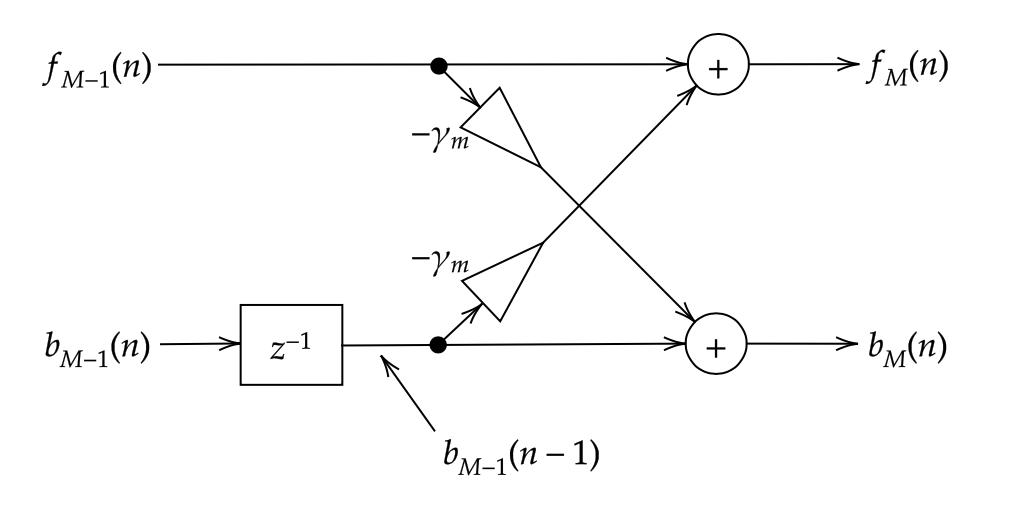
\includegraphics[width=100mm]{./figs/lattice_filter.png}
    \caption{格子型フィルターによる誤差計算} \label{lattice_filter_residual}
  \end{center}
\end{figure}

更に図\ref{cascaded_lattice_filter_residual}の様に、$f_{0}(n) = b_{0}(n) = y(n)$とした上で格子型フィルターを連結することで、任意次数の前向き誤差と後ろ向き誤差を逐次計算できる。
\begin{figure}[htbp]
  \begin{center}
    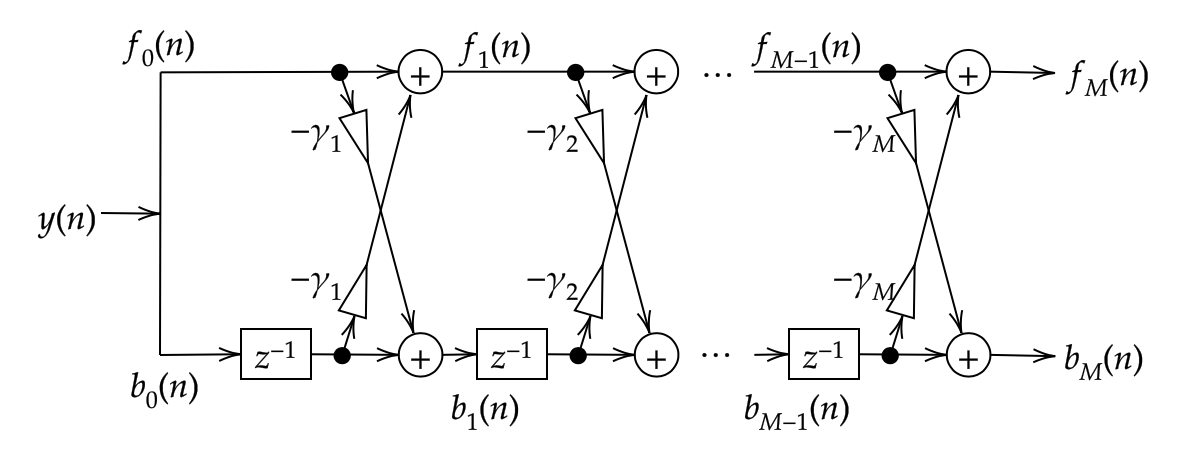
\includegraphics[width=120mm]{./figs/cascaded_lattice_filter_residual.png}
    \caption{格子型フィルターの連結} \label{cascaded_lattice_filter_residual}
  \end{center}
\end{figure}

\subsubsection{PARCOR係数による信号合成}

前向き誤差の式\ref{parcor_forward_residual}の移項操作により、式\ref{parcor_forward_synthesis}のように、より高い次数の前向き誤差$f_{M}(n)$から1つ低い次数の前向き誤差$f_{M-1}(n)$を計算できる。
\begin{eqnarray}
  f_{M-1}(n) &=& f_{M}(n) + \gamma_{M} b_{M-1}(n-1) \label{parcor_forward_synthesis}
\end{eqnarray}

式\ref{parcor_forward_synthesis}の結果は重要である。これは計算済みの前向き誤差$f_{M}(n)$から、式\ref{parcor_forward_synthesis}, \ref{parcor_backward_residual}を繰り返し計算することで元の信号$y(n)$を再合成できることを示している。格子型フィルターとして表現すると図\ref{cascaded_lattice_filter_synthesis}の様に、図\ref{cascaded_lattice_filter_residual}の格子型フィルターの前向き誤差の流れる(計算する)方向を逆転させたフィルターであることが分かる。
\begin{figure}[htbp]
  \begin{center}
    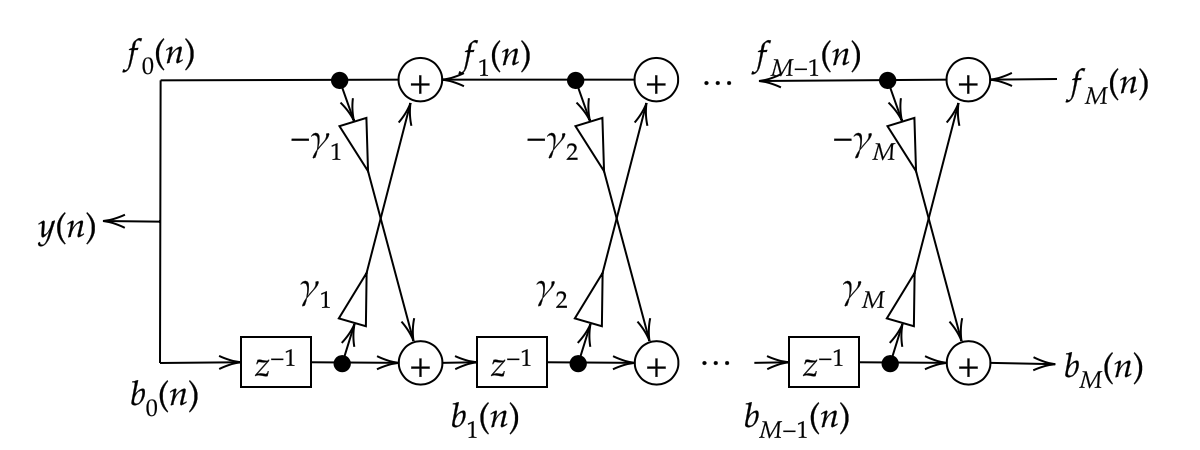
\includegraphics[width=120mm]{./figs/cascaded_lattice_filter_synthesis.png}
    \caption{格子型フィルターによる信号合成} \label{cascaded_lattice_filter_synthesis}
  \end{center}
\end{figure}

\subsubsection{PARCOR係数の値域} \label{range_of_parcor_coef}

式\ref{parcor_forward_residual}, \ref{parcor_backward_residual}を使って再度誤差最小化を考えると、PARCOR係数の値域は$-1 \leq \gamma_{m} \leq 1\ (m=0,\dots,M)$であることが示せる。前向き誤差$f_{m}(n)$の全ての時刻における平均$\textrm{E}$を
\begin{eqnarray*}
  \textrm{E}[f_{m}(n)] = \lim_{N \to \infty}\frac{1}{2N} \sum_{n = -N}^{N} f_{m}(n)
\end{eqnarray*}

で定義すると、前向き誤差の二乗平均$\textrm{E}[f_{m}^{2}(n)]$は次のように展開できる。
\begin{eqnarray*}
  \textrm{E}[f_{m}^{2}(n)] &=& \textrm{E}\left[ \left\{ f_{m-1}(n) - \gamma_{m} b_{m-1}(n - 1) \right\}^{2} \right] \\
  &=& \textrm{E}\left[ f_{m-1}^{2}(n) - 2 \gamma_{m} f_{m-1}(n)b_{m-1}(n - 1) + \gamma_{m}^{2} b_{m-1}^{2}(n - 1) \right] \\
  &=& \textrm{E}\left[ f_{m-1}^{2}(n) \right] - 2 \gamma_{m} \textrm{E}\left[ f_{m-1}(n)b_{m-1}(n - 1) \right] + \gamma_{m}^{2} \textrm{E}\left[ b_{m-1}^{2}(n - 1) \right] 
\end{eqnarray*}

ここで、最後の式変形において平均$\textrm{E}$の線形性を用いている。また、平均$\textrm{E}$は全ての時刻$n$についての平均だから、時刻をシフトして平均をとっても結果は変わらない。従って、$\textrm{E}\left[ b_{m-1}^{2}(n - 1) \right] = \textrm{E}\left[ b_{m-1}^{2}(n) \right]$であること\footnote{$\textrm{E}\left[ f_{m-1}(n)b_{m-1}(n - 1) \right] \neq \textrm{E}\left[ f_{m-1}(n)b_{m-1}(n) \right]$には注意。$\textrm{E}$内の時刻を全て同時にシフトしないと等号は成立しない。例えば、$\textrm{E}[f_{m-1}(n)b_{m-1}(n-1)] = \textrm{E}[f_{m-1}(n+1)b_{m-1}(n)]$は成立する。}により、次の結果を得る。
\begin{eqnarray}
  \textrm{E}[f_{m}^{2}(n)] = \textrm{E}\left[ f_{m-1}^{2}(n) \right] - 2 \gamma_{m} \textrm{E}\left[ f_{m-1}(n)b_{m-1}(n - 1) \right] + \gamma_{m}^{2} \textrm{E}\left[ b_{m-1}^{2}(n) \right] \label{square_of_forward_residual}
\end{eqnarray}

$\textrm{E}[f_{m}^{2}(n)]$を$\gamma_{m}$について偏微分すると、
\begin{eqnarray*}
  \frac{\partial \textrm{E}[f_{m}^{2}(n)]}{\partial \gamma_{m}} = -2 \textrm{E}\left[ f_{m-1}(n)b_{m-1}(n - 1) \right] + 2 \gamma_{m} \textrm{E}\left[ b_{m-1}^{2}(n) \right] 
\end{eqnarray*}

偏微分の結果を$0$とおくことで、PARCOR係数は次の式\ref{another_parcor_coef1}でも求まることが分かる。
\begin{eqnarray} \label{another_parcor_coef1}
  \gamma_{m} = \frac{\textrm{E}\left[ f_{m-1}(n)b_{m-1}(n - 1) \right]}{\textrm{E}\left[ b_{m-1}^{2}(n) \right]}
\end{eqnarray}

更に、後ろ向き誤差$b_{m}(n)$についても、二乗平均$\textrm{E}[b_{m}^{2}(n)]$を$\gamma_{m}$について最小化することで、PARCOR係数は次の式\ref{another_parcor_coef2}でも求まることが分かる。
\begin{eqnarray} \label{another_parcor_coef2}
  \gamma_{m} = \frac{\textrm{E}\left[ f_{m-1}(n)b_{m-1}(n - 1) \right]}{\textrm{E}\left[ f_{m-1}^{2}(n) \right]}
\end{eqnarray}

再度式\ref{square_of_forward_residual}に注目する。この式\ref{square_of_forward_residual}を$\gamma_{m}$に関して平方完成すると、
\begin{eqnarray*}
  \textrm{E}[f_{m}^{2}(n)] &=& \textrm{E}\left[ f_{m-1}^{2}(n) \right] - 2 \gamma_{m} \textrm{E}\left[ f_{m-1}(n)b_{m-1}(n - 1) \right] + \gamma_{m}^{2} \textrm{E}\left[ b_{m-1}^{2}(n) \right] \\
  &=& \textrm{E}\left[ b_{m-1}^{2}(n) \right] \left( \gamma_{m}^{2} - 2\gamma_{m} \frac{\textrm{E}\left[ f_{m-1}(n)b_{m-1}(n - 1) \right]}{\textrm{E}\left[ b_{m-1}^{2}(n) \right]} \right) + \textrm{E}\left[ f_{m-1}^{2}(n) \right] \\
  &=& \textrm{E}\left[ b_{m-1}^{2}(n) \right] \left( \gamma_{m} - \frac{\textrm{E}\left[ f_{m-1}(n)b_{m-1}(n - 1) \right]}{\textrm{E}\left[ b_{m-1}^{2}(n) \right]} \right)^{2} \\
  & & - \frac{\left\{\textrm{E}\left[ f_{m-1}(n)b_{m-1}(n - 1) \right]\right\}^{2}}{\textrm{E}\left[ b_{m-1}^{2}(n) \right]} + \textrm{E}\left[ f_{m-1}^{2}(n) \right] \\
  &=& - \frac{\left\{\textrm{E}\left[ f_{m-1}(n)b_{m-1}(n - 1) \right]\right\}^{2}}{\textrm{E}\left[ b_{m-1}^{2}(n) \right]} + \textrm{E}\left[ f_{m-1}^{2}(n) \right] \quad (\because 式\ref{another_parcor_coef1})
\end{eqnarray*}

ここで、二乗平均は必ず非負$\textrm{E}[f_{m}^{2}(n)] \geq 0$だから、上式は必ず非負でなければならない。非負条件を変形すると、
\begin{eqnarray*}
 && - \frac{\left\{\textrm{E}\left[ f_{m-1}(n)b_{m-1}(n - 1) \right]\right\}^{2}}{\textrm{E}\left[ b_{m-1}^{2}(n) \right]} + \textrm{E}\left[ f_{m-1}^{2}(n) \right] \geq 0 \\
 &\iff& \frac{\left\{\textrm{E}\left[ f_{m-1}(n)b_{m-1}(n - 1) \right]\right\}^{2}}{\textrm{E}\left[ b_{m-1}^{2}(n) \right]} \leq \textrm{E}\left[ f_{m-1}^{2}(n) \right] \\
 &\iff& \frac{\left\{\textrm{E}\left[ f_{m-1}(n)b_{m-1}(n - 1) \right]\right\}^{2}}{\textrm{E}\left[ b_{m-1}^{2}(n) \right] \textrm{E}\left[ f_{m-1}^{2}(n) \right]} \leq 1 \\
 &\iff& \gamma_{m}^{2} \leq 1 \quad (\because 式\ref{another_parcor_coef1}, \ref{another_parcor_coef2})
\end{eqnarray*}

従って、PARCOR係数$\gamma_{m}$の値域が$-1 \leq \gamma_{m} \leq 1$であることが示された。値域が制限されている性質は、符号化を行うにあたって都合が良い。一方、線形予測係数$a_{M}(0), \dots, a_{M}(M)$は値域に制限がなく、符号化の際に係数範囲についての追加情報を必要とする。

\subsection{線形予測の実装} \label{lpc_example_impl}

Levinson-Durbin法のC言語による実装をリスト\ref{lpc_example}に示す。
\lstinputlisting[caption=Levinson-Durbin再帰法の実装例,label=lpc_example]{./example_src/lpc_example.c}

\subsubsection{実験}

実際にリスト\ref{lpc_example}を実行し、元の信号と予測した信号をプロットしたグラフを図\ref{lpc_test_result}に示す。
\begin{figure}[htbp]
  \begin{center}
    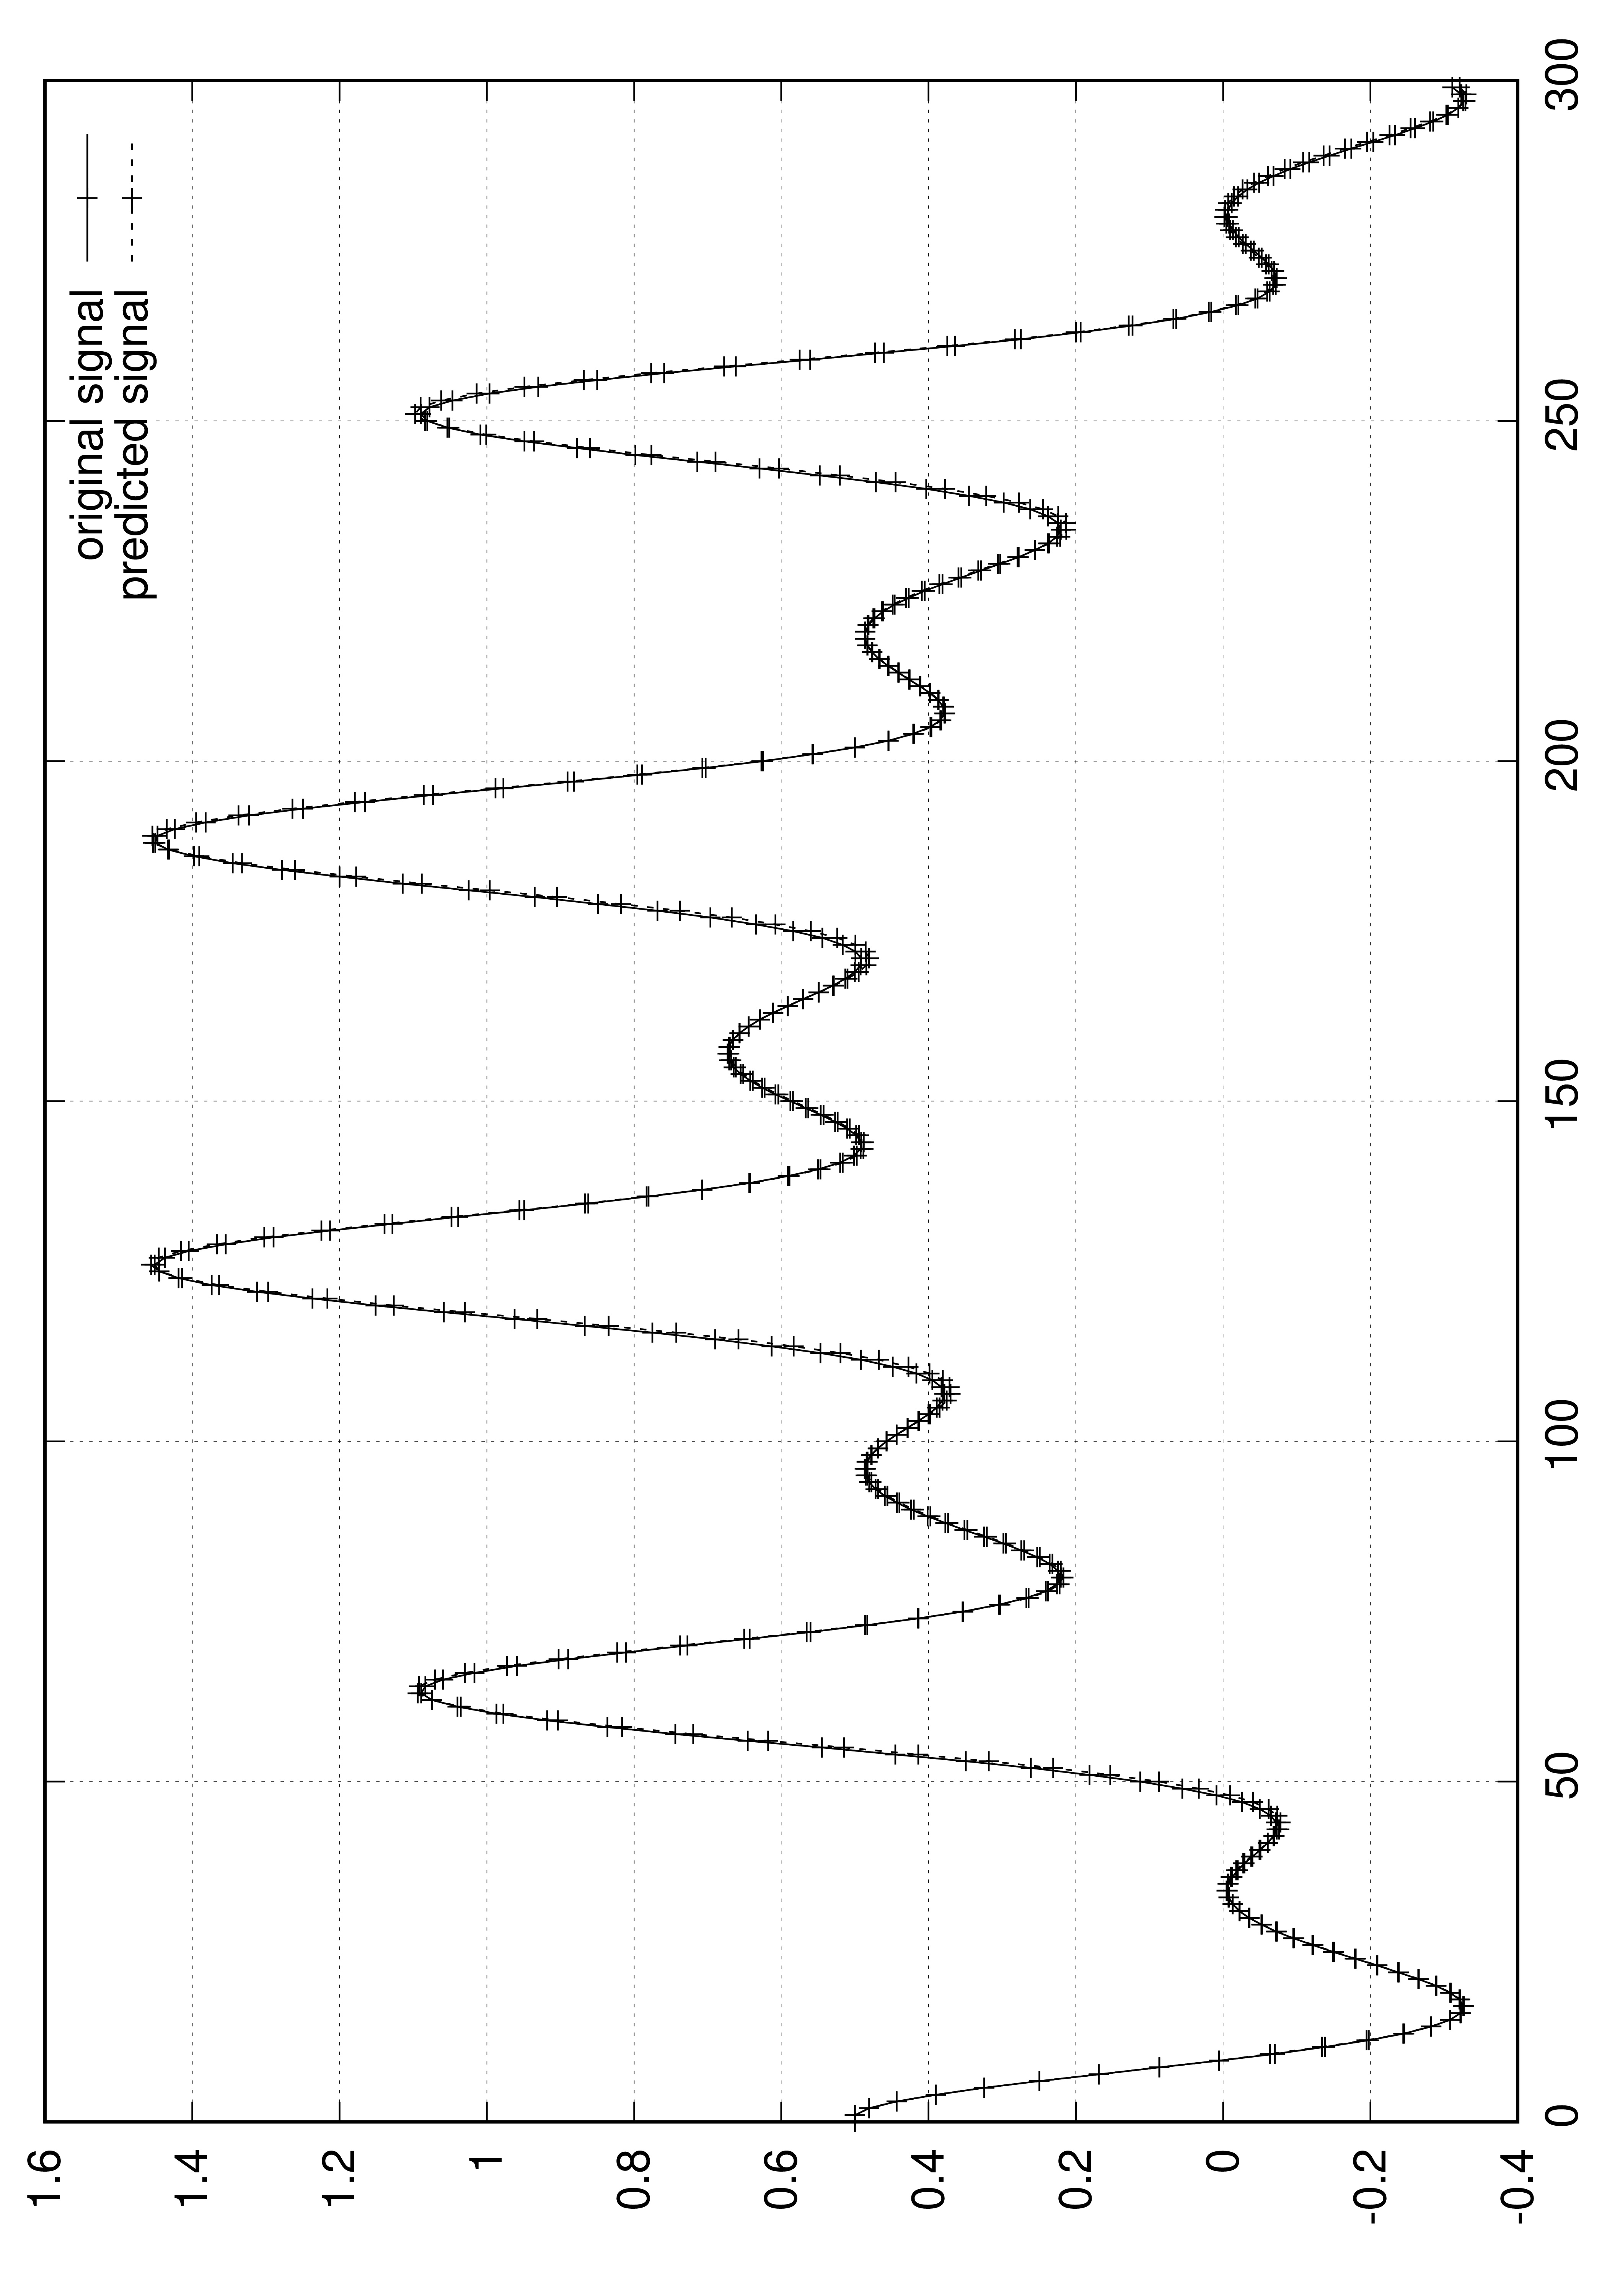
\includegraphics[width=60mm,angle=-90]{./figs/lpc_test_result.png}
    \caption{リスト\ref{lpc_example}の実行結果} \label{lpc_test_result}
  \end{center}
\end{figure}

原信号が簡単すぎたのか、元の信号と予測した信号はほぼ重なっており、係数は少なめでも十分に予測できている事が分かる。

\section{エントロピー符号}

データ圧縮においては、圧縮後のサイズを小さくするために、いかに情報を短く符号化できるかが重要になる。短い符号化を達成するためには、原理的には情報をくまなく観察し、頻繁に登場する情報のパターンに対して短い符号を割り当ててやれば良い。

例えば、英語のアルファベットの中では'e'が最も出現確率が高いという統計\cite{alphabethist}がある。このパターンを利用して、'e'に短い符号を割り当てれば英単語を効率的に圧縮することができる。この様に、情報の中に潜んでいるパターンの\textbf{確率}を基に符号化を行う手法を\textbf{エントロピー符号化(entropy coding)}\index{えんとろぴーふごうか@エントロピー符号化}という。

本節では、\cite{amariinfo,miyagawainfo}を参考に、情報とその定量的基準の定義と、ロスレス音声コーデックでしばしば使われるエントロピー符号の例を見ていく。

\subsection{情報とその符号化\label{information_and_coding}}

我々の住む世界には様々な\textbf{情報(information)}\index{じょうほう@情報}が溢れている。国語辞典\cite{kokugojiten}を紐解くと、情報とは「事件や物事の内容や様子についての知らせ」と定義されている。例えば、人間同士の会話は事件や物事の知らせになっているので情報であるし、今読んでいるこの文章も何らかの技術を知らせるものであるから、情報の一つである。

情報理論では、情報は情報を発する源、つまり\textbf{情報源(information source)}\index{じょうほうげん@情報源}から生起(発生)するものと捉えている。また、生起した情報の時間的な系列は、過去に生起した情報に(確率的に)依存して生起すると考えられる。例えば、良くシャッフルされたトランプの山札からカードを一枚ずつ引いていく時、引いたカードに応じて残りのカードを引く確率が変動し、これから引くカード、即ち情報の生起が定まってくる。

\textbf{符号化(coding, encoding)(エンコード)}\index{ふごうか@符号化}\index{えんこーど@エンコード}とは、情報を一定の規則に従って変換する(言い換える)ことを指す。また、符号化の変換規則を\textbf{符号(code)}\index{ふごう@符号}という。例として、4つのアルファベット$A, B, C, D$を$0,1$の列に割当てる符号を次のように定義する。
\begin{eqnarray*}
  A &\rightarrow& 00 \\
  B &\rightarrow& 01 \\
  C &\rightarrow& 10 \\
  D &\rightarrow& 11
\end{eqnarray*}
この符号を用いてアルファベットの列$AABD$を符号化すると、
\begin{eqnarray*}
  AABD &\rightarrow& 00\ 00\ 01\ 11
\end{eqnarray*}
という列が得られる。符号化したままでは元の情報の内容は分からないので、符号の逆の対応規則
\begin{eqnarray*}
  00 &\rightarrow& A \\
  01 &\rightarrow& B \\
  10 &\rightarrow& C \\
  11 &\rightarrow& D
\end{eqnarray*}
によって列$00\ 00\ 01\ 11$を戻すと、
\begin{eqnarray*}
  00\ 00\ 01\ 11 &\rightarrow& AABD
\end{eqnarray*}
元の情報に戻ることが分かる。この様に、符号化された情報を元の情報に戻す操作を\textbf{復号(decoding)(デコード)}\index{ふくごう@復号}\index{でこーど@デコード}という。

\subsubsection{一意に復号可能な符号}

情報源を符号化するにあたって、符号が曖昧さを残さずに復号できる性質は実用上非常に重要である。何故なら、符号化した情報を受け取ったときに、それを完全に元の情報に復号できなければ、情報を正しく伝達できたとは言えないからである。本節では、曖昧さを残さずに復号できる符号の性質を見ていく。

議論に立ち入る前に、符号についての用語定義を行っておく。まず、符号語の数が$r$個ある符号を$r$元符号という。例えば、$0, 1$から構成される符号は$r=2$で2元符号である\footnote{2元符号のことを特にバイナリコード(binay code)と呼ぶこともある。}。また、符号の列が与えられた時、それを一意に(ただ一通りの方法で)復号できる符号を\textbf{一意に復号可能な符号(uniquely decodable code)}\index{いちいふくごうかのうな符号@一意に復号可能な符号}という。一意に復号可能な符号とそうでない(一意に復号不可能な)2元符号の例を表\ref{examples_of_binary_code}に挙げる。

\begin{table}[htbp]
  \begin{center}
    \caption{2元符号の例} \label{examples_of_binary_code}
    \begin{tabular}{c|c|c|c}
      記号 & 符号1 & 符号2 & 符号3 \\ \hline
      $A$  & $00$  & $0$   & $0$   \\
      $B$  & $01$  & $1$   & $01$  \\
      $C$  & $10$  & $0$   & $10$  \\
      $D$  & $11$  & $1$   & $11$  \\
    \end{tabular}
  \end{center}
\end{table}

表\ref{examples_of_binary_code}に挙げた符号1,2,3について、一意に復号可能かどうかを観察すると、

\begin{description}
    \item[符号1] 一意に復号可能な符号である。全ての符号の列は、2文字ずつ区切れば、$A, B, C, D$のいずれかに重複なく対応付けることができる。
    \item[符号2] 一意に復号不可能な符号である。$0$だけを見た時、それが元の記号が$A$だったのか、$C$だったのかを区別できない。同様に、$1$だけを見たときも$B, D$で区別できない。
    \item[符号3] 一意に復号不可能な符号である。符号の列$"0110"$を見た時、
      \begin{eqnarray*}
        0110 &\to& ADA \\
        0110 &\to& BC
      \end{eqnarray*}
      という様に、2通りに復号できてしまう。
\end{description}

\subsubsection{McMillan(マクミラン)の不等式}

一意に復号可能な符号が持つ性質を特徴付ける定理として、次の\textbf{マクミランの不等式(McMillan inequality)}\index{まくみらんのふとうしき@マクミランの不等式}がある。

\begin{theorem}[マクミランの不等式] \label{mcmillan_ineqality}
  $r$元符号が一意に復号可能ならば、記号の数$q$に対応する符号の長さの組$l_{1}, l_{2}, \dots, l_{q}$は、次の不等式を満たす。
  \begin{eqnarray}
    \sum_{i = 1}^{q} r^{-l_{i}} \leq 1
  \end{eqnarray}
\end{theorem}

\begin{proof}
  不等式の右辺は何乗しても$1$のままであることを使い、任意の自然数$n$に対して$(\sum_{i=1}^{q} r^{-l_{i}})^{n} \leq 1$を示す。左辺の$(\sum_{i=1}^{q} r^{-l_{i}})^{n}$を展開すると、各項は$r^{-l_{1}}, r^{-l_{2}}, \dots, r^{-l_{q}}$から$n$回選択して乗じた項の和だから、$r^{-l_{j}}$を選択したことを$i_{j}$と表すと、$n$回の乗算の選択を以下の式のように表せる。
  \begin{eqnarray*}
    r^{-l_{i_{1}}} \times r^{-l_{i_{2}}} \dots \times r^{-l_{i_{n}}} 
  \end{eqnarray*}
  今、$r^{-l_{i_{1}}}, r^{-l_{i_{2}}}, \dots, r^{-l_{i_{n}}}$を選択したときの符号列の長さを$j = l_{i_{1}} + l_{i_{2}} + \dots + l_{i_{n}}$とおけば、
  \begin{eqnarray*}
    r^{-j} = r^{-l_{i_{1}}} \times r^{-l_{i_{2}}} \dots \times r^{-l_{i_{n}}} 
  \end{eqnarray*}
  と表せる。こうした上で、$l_{\min}, l_{\max}$をそれぞれ$l_{1}, \dots, l_{q}$の最小値と最大値とすると、$l_{\min} \leq l_{i_{1}}, l_{i_{2}}, \dots, l_{i_{n}} \leq l_{\max}$だから、$nl_{\min} \leq j \leq nl_{\max}$が成立する。これにより、
  \begin{eqnarray} \label{n_times_mult_mcmillan}
    \left( \sum_{i=1}^{q} r^{-l_{i}} \right)^{n} = \sum_{j = nl_{\min}}^{nl_{\max}} w_{j} r^{-j}
  \end{eqnarray}
  と表せる。ここで、$w_{j}$は長さ$n$の記号を符号化したときに、長さが$j$になるような符号の組み合わせ数である。
  構成した符号によっては、符号化したときの長さとして実現できない長さ$j$が存在するが、そのような長さ$j$については$w_{j} = 0$とおく
  \footnote{$w_{j}$は多項係数から求められる。長さ$l_{i}$の符号を選んだ回数を$k_{i} \geq 0$と書くと、
  \begin{eqnarray*} 
    w_{j} = \frac{n!}{k_{1}!k_{2}!\dots k_{q}!}
  \end{eqnarray*} 
  となる。ここで、$j = k_{1}l_{1} + l_{2}l_{2} + \dots + k_{q}l_{q}$が成り立っている。$j = k_{1}l_{1} + l_{2}l_{2} + \dots + k_{q}l_{q}$を成り立たせる$k_{i} (i = 1,\dots,q)$の組み合わせが存在しない場合は、その長さ$j$を持つ符号列は出現しないから$w_{j} = 0$となる。}。
  更に$w_{j}$について注目する。長さ$j$の符号の列について、$r^{j}$は長さ$j$の$r$元符号が表現できる最大の記号数だから、不等式
  \begin{eqnarray} \label{ineq_of_combination_of_codes}
    w_{j} \leq r^{j}
  \end{eqnarray} 
  % 長さ$j$の符号列について$r^{j}$は長さ$j$の符号列の最大値を示している
  % 符号列の重複を許す順列の数になっており、$r^{j}$通りより大きい組み合わせ数は無いことがわかり、次の不等式が成立する。
  が成立する。逆に$w_{j} > r^{j}$と仮定すると、長さ$j$の符号列の組み合わせに重複が発生してしまうから、一意に復号可能な符号の仮定に反する。\footnote{例えば、2元符号$0,1$からなる長さ1の符号を考えてみる。この場合は$r=2, j=1$で$r^{j}=2^{1}=2$となる。一方$w_{1}$は定義により長さ$1$の符号列の組み合わせを意味している。もし$w_{1} = 3$ならば、これは、長さ1の符号列が3通り存在することになる。しかし、長さ1の2元符号では、$0,1$の2通りしか符号の列が存在しない。3通り目以上の符号の列を考えると、長さ1において$0,1$のいずれかを使わざるを得ない。即ち、必ず重複が生じてしまい、その符号は一意に復号不可能になる。従って、2元符号が一意に復号可能であるためには$w_{1} \leq 2$でなくてはならない。}
  この不等式\ref{ineq_of_combination_of_codes}を式$\ref{n_times_mult_mcmillan}$に代入すると、
  \begin{eqnarray*}
    \left( \sum_{i=1}^{q} r^{-l_{i}} \right)^{n} &=& \sum_{j = nl_{\min}}^{nl_{\max}} w_{j} r^{-j} \\
    &\leq& \sum_{j = nl_{\min}}^{nl_{\max}} r^{j} r^{-j} = \sum_{j = nl_{\min}}^{nl_{\max}} 1 = nl_{\max} - nl_{\min} + 1 \\
    &\leq& nl_{\max}
  \end{eqnarray*}
  が導かれる。$(\sum_{i=1}^{q} r^{-l_{i}})^{n} > 1$のとき、$n$を大きくしていくと左辺$(\sum_{i=1}^{q} r^{-l_{i}})^{n}$は指数的に増加するのに対し、右辺$nl_{\max}$は線形にしか増加していかないので、不等式は成立しなくなる。従って、任意の自然数$n$に対して不等式が成立するためには、
  \begin{eqnarray*}
    \displaystyle\left( \sum_{i=1}^{q} r^{-l_{i}} \right)^{n} \leq 1
  \end{eqnarray*}
  でなければならない。この不等式を成り立たせる条件として、マクミランの不等式
  \begin{eqnarray*}
    \sum_{i=1}^{q} r^{-l_{i}} \leq 1
  \end{eqnarray*}
  が得られる。
\end{proof}

定理\ref{mcmillan_ineqality}の命題の対偶「$\sum_{i=1}^{q}r^{-l_{i}} > 1$ならば、符号は一意に復号不可能」を用いることで、構成した符号が一意に復号不可能な符号なのか判定できる\footnote{定理\ref{mcmillan_ineqality}の命題の逆、即ち「$\sum_{i=1}^{q}r^{-l_{i}} \leq 1$ならば、符号は一意に復号可能」は、\textbf{クラフトの不等式(Kraft's inequality)}から導き出すことができる。この結果により、実は$\sum_{i=1}^{q}r^{-l_{i}} \leq 1$が一意に復号可能な符号の必要十分条件であることが示せる。本稿では証明しない。}。表\ref{examples_of_binary_code}で挙げた符号について、一意に復号不可能な符号を正しく判定できているか判定してみると、次の結果が得られる。
\begin{description}
  \item[符号2] $r = 2,\ l_{i} = 1\ (i = 1,2,3,4)$だから、
      \begin{eqnarray*}
        \sum_{i = 1}^{q} r^{-l_{i}} = \sum_{i = 1}^{4} 2^{-l_{i}} = 2^{-1} + 2^{-1} + 2^{-1} + 2^{-1} = 2 > 1
      \end{eqnarray*}
      よって一意に復号不可能。
  \item[符号3] $r = 2,\ l_{1} = 1,\ l_{2} = 2,\ l_{3} = 2,\ l_{4} = 2$だから、
      \begin{eqnarray*}
        \sum_{i = 1}^{q} r^{-l_{i}} = \sum_{i = 1}^{4} 2^{-l_{i}} = 2^{-1} + 2^{-2} + 2^{-2} + 2^{-2} = \frac{5}{4} > 1
      \end{eqnarray*}
      よって一意に復号不可能。
\end{description}

簡単な例において、マクミランの不等式が成立していることが確かめられる。

\subsection{情報量とエントロピー}

\ref{information_and_coding}節で触れた情報を定量的に扱う尺度として\textbf{情報量}\index{じょうほうりょう@情報量}がある。情報量は、特定の情報の知らせを得ることで、不確実性がどの程度減少したかという尺度に基づいて測ることができる。不確実性を定性的に扱うには\textbf{確率}を使用する。本節では、情報量と、不確実性を定量的に扱う概念であるエントロピーについて見ていく。

\subsubsection{情報量の定義}

最初に、情報量の形式的な定義を与える。

\begin{definition}[情報量]
  事象$A$が生起したことを知ったときに得られる情報量を$I(A)$を書くと、情報量は式\ref{information_amount}で定義される。
  \begin{eqnarray}
    I(A) = -\log_{2} P(A) \quad [bit] \label{information_amount}
  \end{eqnarray}
  ここで、$P(A)$は事象$A$の生起する確率である。
\end{definition}

なぜ情報量がこの式\ref{information_amount}の形で与えられるのかは後術する。まずは、情報量の計算例をいくつか挙げることで、情報量が直感的に妥当な尺度になっていることを観察する。

\begin{example}[コイン投げ]
  イカサマの無いコインを投げる事を考える。コイン投げによって得られる結果は、「コインの表が出る」か「コインの裏が出る」の2通りしかありえない\footnote{コインが縁で直立することは無いものとする。}。コインの表が出る確率を$P(表)$, 裏が出る確率を$P(裏)$と書くとすると、$P(表) = P(裏) = 1/2$である。従って、コインの表が出たことを知ったときに得られる情報量$I(表)$は次のように計算できる:
  \begin{eqnarray*}
    I(表) = - \log_{2} P(表) = -\log_{2} \frac{1}{2} = \log_{2} 2 = 1
  \end{eqnarray*}
  即ち、コインを投げてその結果を確認することで$1[bit]$の情報が得られる。例えば、コインの表を1、裏を0に対応付けることで、確かに1bitでコインの表裏の情報をもれなく保存できるから、コイン投げによる情報量が1bitとなるのはもっともである。
\end{example}

\begin{example}[2枚のコイン投げ] \label{information_example2}
  2枚のコインを同時に投げる事を考える。$P(1枚目が表) = P(2枚目が表) = 1/2$であり、各々のコインの表と裏が出る確率は、各々のコイン投げの結果に影響を及ぼさない、つまり\textbf{独立}だから、次の式が成り立つ。
  \begin{eqnarray*}
    P(1枚目が表かつ2枚目が表) = P(1枚目が表)P(2枚目が表) = \frac{1}{2} \times \frac{1}{2} = \frac{1}{4}
  \end{eqnarray*}
  このように確率計算が分解できることを踏まえた上で、2枚のコインを投げ、2枚とも表だと知ったときに得られる情報量を計算すると、
  \begin{eqnarray}
    I(1枚目が表かつ2枚目が表) &=& -\log_{2} P(1枚目が表かつ2枚目が表) \nonumber \\
    &=& -\log_{2} P(1枚目が表) P(2枚目が表) \nonumber \\
    &=& -\log_{2} P(1枚目が表) - \log_{2} P(2枚目が表) \nonumber \\
    &=& I(1枚目が表) + I(2枚目が表) \label{information_additive} \\
    &=& 2 \nonumber
  \end{eqnarray}
  よって、2枚のコインを同時に投げて、その結果を確認することで$2[bit]$の情報が得られる。また、式\ref{information_additive}に注目すると、全体の情報量が、各々のコインの表裏を確認するときに得られる情報量の和に分解されていることが分かる。これは、情報量の持つ\textbf{加法性}を示している。
\end{example}

\subsubsection{情報量の導出}

情報量が式\ref{information_amount}の形で与えられるのは、例\ref{information_example2}で触れた情報量の加法性から自然に導かれる。ここでは\cite{amariinfo}を参考に導出を行う。$x$通りの事象がすべて等確率で生起する情報源の情報量を$I(x)$と表す。加法性により、$x,y$通りの事象が互いに独立ならば、
\begin{eqnarray}
  I(xy) = I(x) + I(y) \label{information_add}
\end{eqnarray}

が成立する\footnote{例\ref{information_example2}で挙げたコイン投げの例では、2枚のコインを投げる事象は全4通り、1枚のコインを投げる事象は全2通りだから、$I(4) = I(2) + I(2)$となっている。}。また、1通りの事象しか生起しない場合の情報量は0、即ち、
\begin{eqnarray}
  I(1) = 0  \label{information_zero}
\end{eqnarray}

が成立する。1通りの事象しか生起しない場合、情報の知らせを受けなくても何が起きるか分かってしまうので、その場合の情報量が0になるのはもっともである。

これらの前提(式\ref{information_add}, \ref{information_zero})の元で、定数$\varepsilon$を用いて$I(x+\varepsilon x)$を計算すると、
\begin{eqnarray}
  I(x + \varepsilon x) &=& I((1 + \varepsilon) x) \nonumber \\
  &=& I(1 + \varepsilon) + I(x) \nonumber \\
  \iff I(x + \varepsilon x) - I(x) &=& I(1 + \varepsilon) \label{information_additive_x_p_ex}
\end{eqnarray}

式\ref{information_additive_x_p_ex}の両辺を$\varepsilon x$で割ると、
\begin{eqnarray}
  \frac{I(x + \varepsilon x) - I(x)}{\varepsilon x} = \frac{1}{x} \frac{I(1 + \varepsilon)}{\varepsilon} \label{pre_diff_information}
\end{eqnarray}

なる関係式が得られる。ここで、$\varepsilon \to 0$の極限をとると、式\ref{pre_diff_information}の左辺は$I(x)$の導関数$I^{\prime}(x)$そのものとなる。右辺の$I(1+\varepsilon)/\varepsilon$は、分子分母共に$0$に近づいていくが、その極限値を$c$とおく:
\begin{eqnarray*}
  \lim_{\varepsilon \to 0} \frac{I(1+\varepsilon)}{\varepsilon} = c
\end{eqnarray*}

$I^{\prime}(x)$と$c$を用いて式\ref{pre_diff_information}を書き直すと、
\begin{eqnarray*}
  I^{\prime}(x) = \frac{c}{x}
\end{eqnarray*}

となる。更に、両辺の不定積分を計算すると、
\begin{eqnarray*}
  \int I^{\prime}(x) \textrm{d}x &=& \int \frac{c}{x} \textrm{d}x \\
  \implies I(x) &=& c \log x + d \quad (d: 積分定数)
\end{eqnarray*}

となり、対数$\log$が現れる。次に、$c,d$が不定なので決定することを考える。まず、前提$I(1) = 0$(式\ref{information_zero})より、
\begin{eqnarray*}
  I(1) = c \log 1 + d = 0 \, \implies \, d = 0
\end{eqnarray*}

また、コイン投げの例で観察したように、2つの情報が等確率で生起する時を情報量の基本単位とし、$I(2) = 1[bit]$と定めると、
\begin{eqnarray*}
  I(2) = c \log 2 = 1 \, \implies \, c = \frac{1}{\log 2}
\end{eqnarray*}

従って、$x$個からなる事象の情報量$I(x)$は次の式で表せる:
\begin{eqnarray} \label{uniform_information}
  I(x) = \frac{\log x}{\log 2} = \log_{2} x
\end{eqnarray}

次に、式\ref{uniform_information}を用いることで、一般の情報量の定義(式\ref{information_amount})が得られることを見ていく。式\ref{uniform_information}により、$n$個の事象が等確率に生起する情報源から得られる情報量は$I(n) = \log_{2} n$である。一方、$n$個の事象の中から$k$個をまとめて$B$とおくと、$B$の部分が持つ情報量は$I(k) = \log_{2} k$となる。

$B$の中から何かの事象が生起したと分かったとしても、$n$個全体の中では何が生起したのかは確定しない。何が生起したのかを確定させるためには、$I(k)$に加え$B$の中から何が生起したのかを確定させる情報量$I(B)$が必要である。このことを式に表すと、
\begin{eqnarray*}
  I(k) + I(B) &=& I(n) \\
  \log_{2} k + I(B) &=& \log_{2} n \\
  \implies I(B) &=& \log_{2} n - \log_{2} k = - \log_{2} \frac{k}{n} 
\end{eqnarray*}

上式において$k/n$は$B$が生起する確率、即ち$P(B)$に他ならない。従って、
\begin{eqnarray*}
  I(B) = - \log_{2} P(B)
\end{eqnarray*}

となって、情報量の定義式\ref{information_amount}が情報量の加法性から自然に導かれることが確かめられた。

\subsubsection{エントロピー}

\textbf{エントロピー(entropy)}\index{えんとろぴー@エントロピー}という言葉は熱力学から来ており、力学系の不確定度(無秩序)の度合いを表す量のことを指す。情報理論においてエントロピーは、情報量の\textbf{期待値}として定義される。

\begin{definition}[エントロピー]
  $n$個の事象$A_{1}, A_{2}, \dots, A_{n}$が存在する時、エントロピー$H(A)$は式\ref{entropy}で定義される。
  \begin{eqnarray}
    H(A) = -\sum_{i = 1}^{n} P(A_{i}) \log_{2} P(A_{i}) \label{entropy}
  \end{eqnarray}
  ここで$P(A_{i})$は$A_{i}$の生起する確率である。
\end{definition}

後術するが、エントロピーは符号の長さに関する非常に重要な性質を持つ。また定義上、エントロピーは\textbf{期待値}であることを強調しておきたい。情報量は情報の知らせを受けてから確定する量である。一方、エントロピーは、情報の知らせを受ける\textbf{前}にどれほどの情報量が得られるかを推定する量となる。

\begin{example}[サイコロ投げ] \label{dice6_roll}
イカサマがなく、全ての面が等確率で生起する六面サイコロを振る時、そのエントロピー$H$は次のように計算できる:
\begin{eqnarray*}
  H &=& - \sum_{i = 1}^{6} P(サイコロの出目がi) \log_{2} P(サイコロの出目がi) \\
  &=& - \sum_{i = 1}^{6} \frac{1}{6} \log_{2} \frac{1}{6} = -\log_{2} \frac{1}{6} = \log_{2} 6 
\end{eqnarray*}
\end{example}

例\ref{dice6_roll}では全ての事象が等確率で生起する例を見た。
この「全て等確率」という状況は確率に偏りが無く、最も予測のしづらい、言い換えると不確定度が最も高い状況であると言える。その性質を正確に表現した、エントロピーの重要な定理が存在する。
\begin{theorem} \label{max_entropy}
  $n$個の事象を持つ情報源のエントロピーの最大値$H$は、
  \begin{eqnarray}
    H = \log_{2} n \quad [bit]
  \end{eqnarray}
  で、それは、全ての事象が等確率$\displaystyle\frac{1}{n}$で生起するときのエントロピーである。
\end{theorem}

\begin{proof}
  $n$個の全ての事象が$1/n$の確率で生起するならば、エントロピー$H$は定義により、
  \begin{eqnarray*}
    H = -\sum_{i = 1}^{n} \frac{1}{n} \log_{2} \frac{1}{n} = \log_{2} n
  \end{eqnarray*}
  と計算できる。この値が最大値であることを示すには、$P_{i} \geq 0,\ \sum_{i = 1}^{n} P_{i} = 1$となるような任意の確率分布$P_{1},\dots,P_{n}$からなる情報源のエントロピーよりも$\log_{2} n$の方が大きいこと、即ち、
  \begin{eqnarray*}
    -\sum_{i = 1}^{n} P_{i} \log_{2} P_{i} \leq \log_{2} n
  \end{eqnarray*}
  が成立することを示せば良い。上式の不等式において、左辺から右辺を減じると、
  \begin{eqnarray*}
    -\sum_{i = 1}^{n} P_{i} \log_{2} P_{i} - \log_{2} n &=& \sum_{i = 1}^{n} P_{i} \log_{2} \frac{1}{P_{i}} + \log_{2} \frac{1}{n} \\
    &=& \sum_{i = 1}^{n} P_{i} \log_{2} \frac{1}{P_{i}} + \sum_{i = 1}^{n} P_{i} \log_{2} \frac{1}{n}  \\
    &=& \sum_{i = 1}^{n} P_{i} \log_{2} \frac{1}{n P_{i}} \\
    &=& \frac{1}{\log 2} \sum_{i = 1}^{n} P_{i} \log \frac{1}{n P_{i}}
  \end{eqnarray*}
  ここで、対数関数に関する次の不等式を適用する。
  \begin{eqnarray} 
    \log x \leq x - 1 \label{log_function_characteristics}
  \end{eqnarray}
  この不等式の成立は、図\ref{xandlogx}に示したグラフからも明らかである\footnote{念の為解析的に証明する。$f(x) = x-1-\log x$を微分すると、$f^{\prime}(x) = 1 - \frac{1}{x}$となる。$f^{\prime}(x) = 0$を$x$について解くと$x=1$が得られ、$f(x)$は$x=1$で極点を持つ。$f(1) = 0$であり、$x < 1$では$f(x) > 0$かつ$f^{\prime}(x) < 0$、$x > 1$では$f^{\prime}(x) > 0$であることから、$f(x)$は$x=1$において最小値$0$を取ることが分かる。即ち、$f(x) = x-1-\log x \geq 0 \iff x-1 \geq \log x $が成立する。}。
  \begin{figure}[htbp]
    \begin{center}
      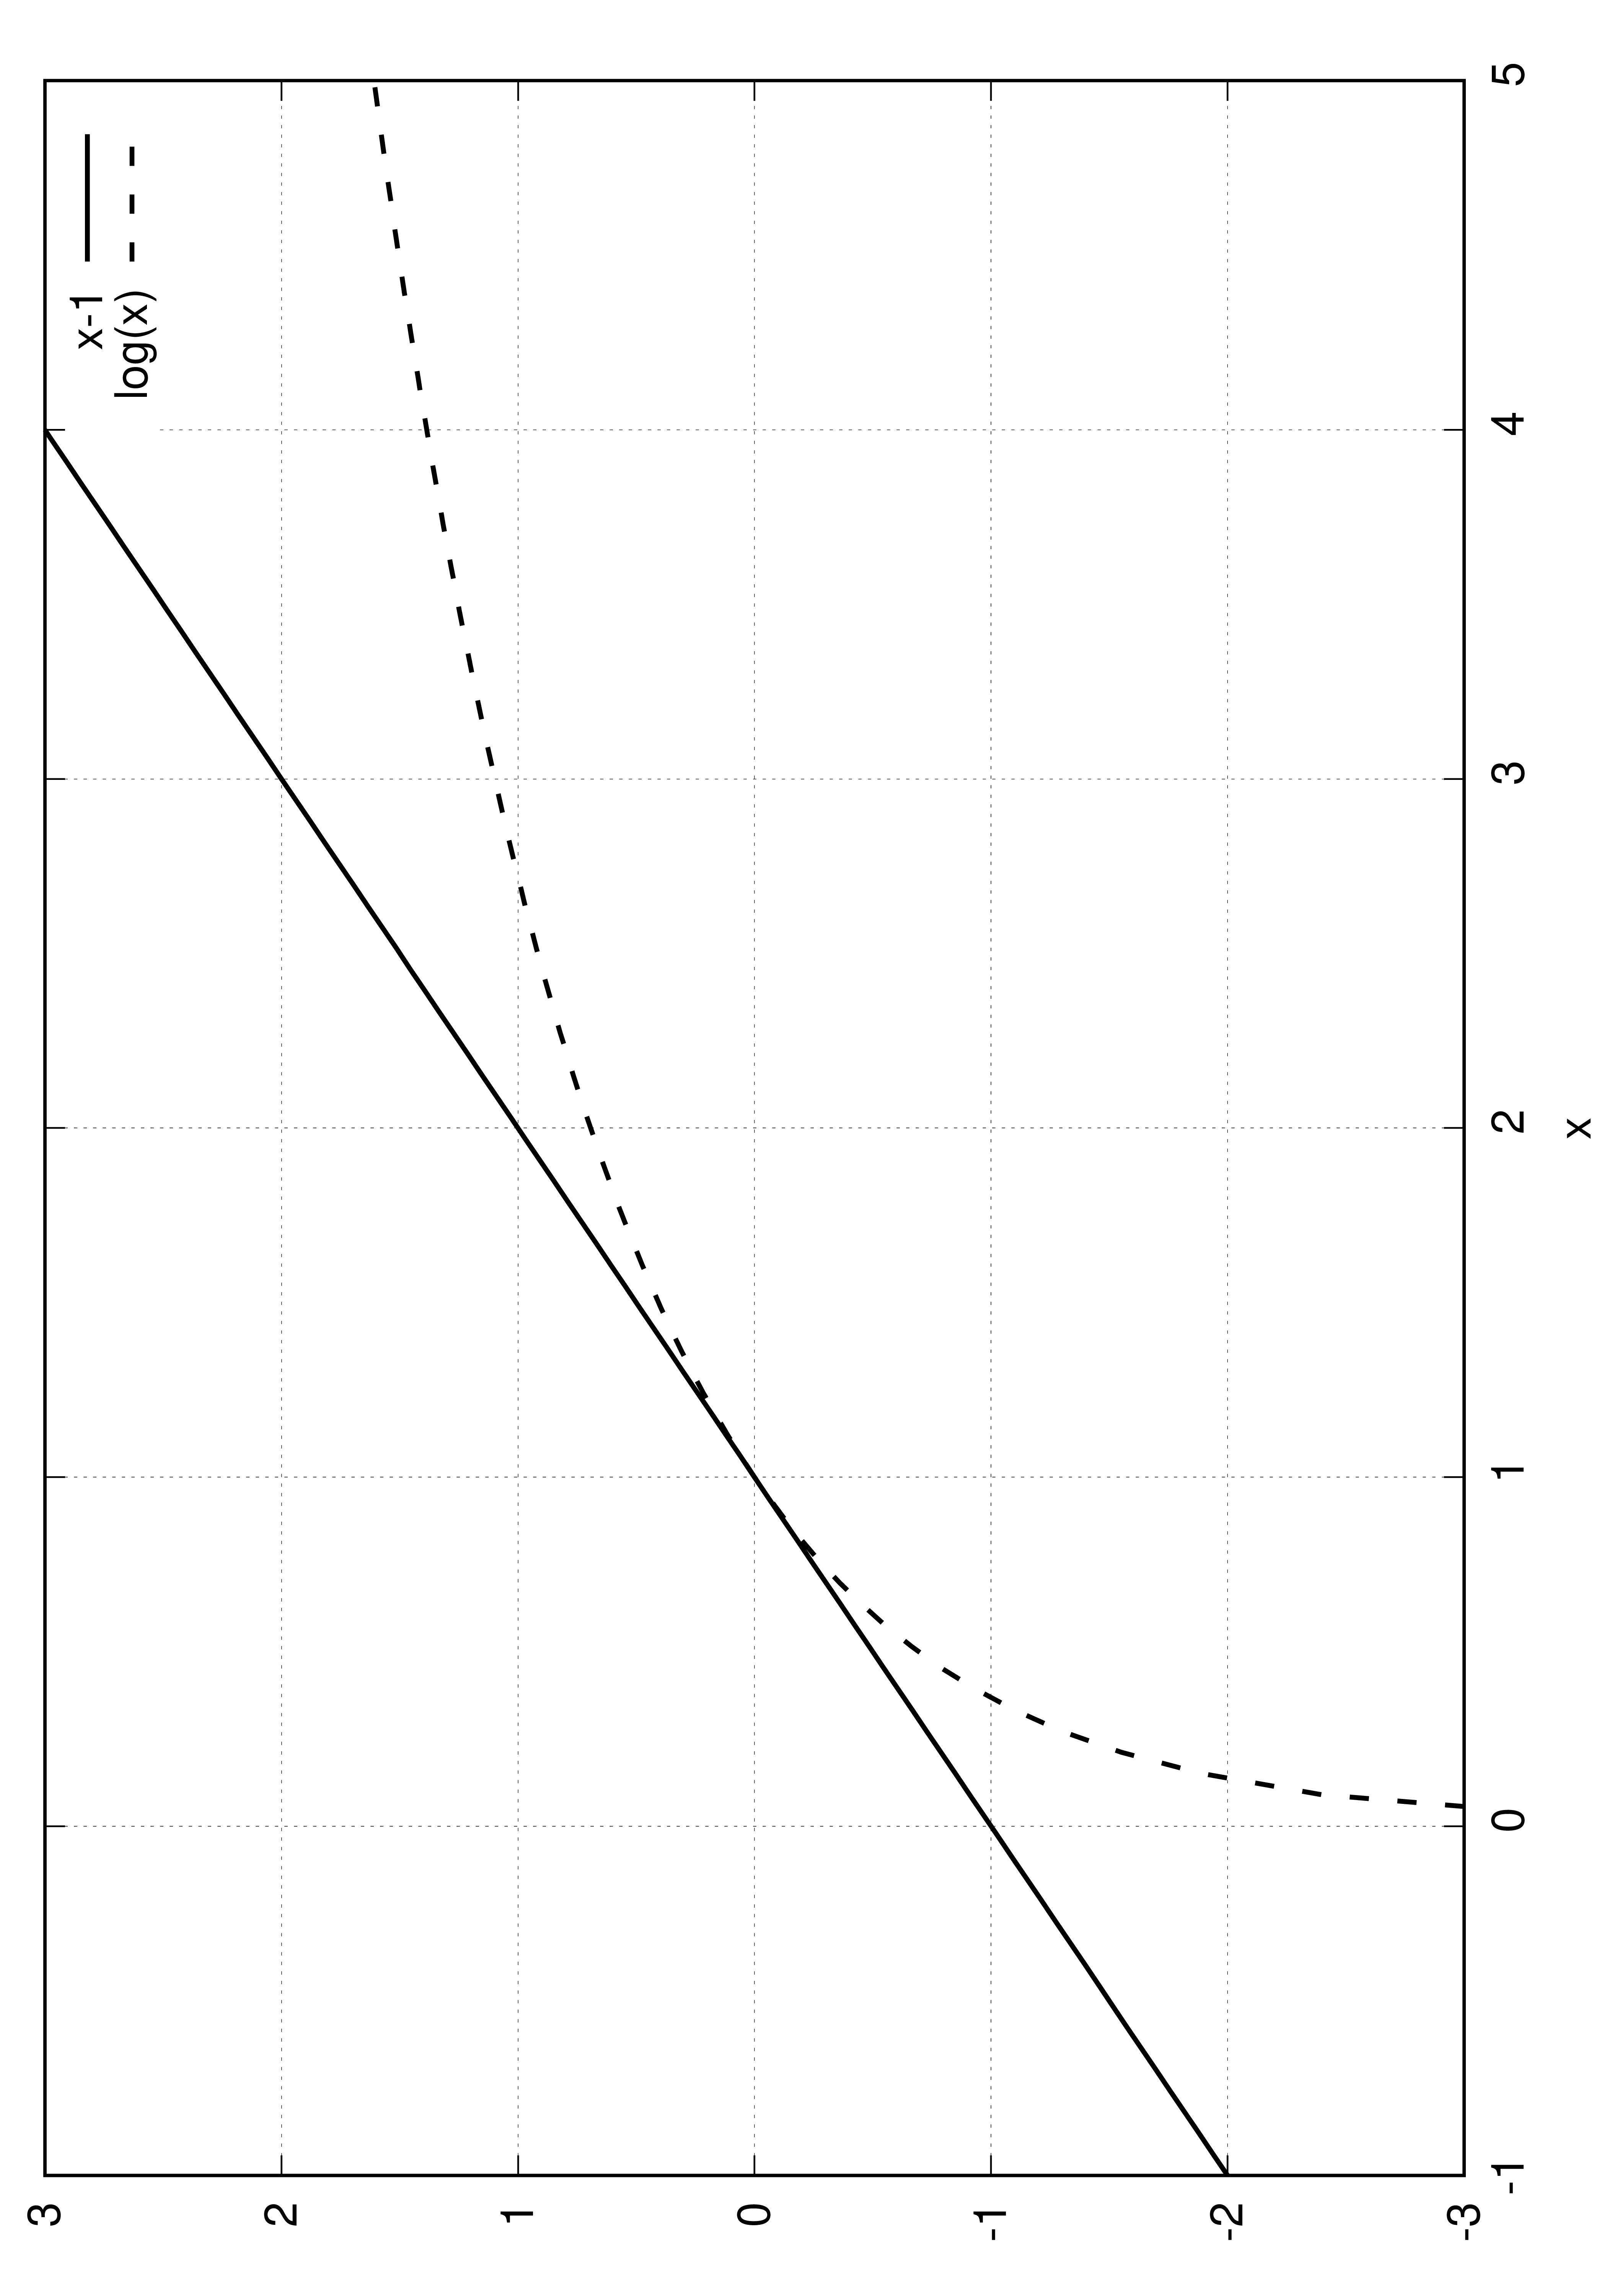
\includegraphics[width=60mm,angle=-90]{./figs/x-1_logx.png}
      \caption{$x - 1$と$\log x$のグラフ} \label{xandlogx}
    \end{center}
  \end{figure}
  不等式を適用すると、
  \begin{eqnarray*}
    -\sum_{i = 1}^{n} P_{i} \log_{2} P_{i} - \log_{2} n &=& \frac{1}{\log 2} \sum_{i = 1}^{n} P_{i} \log \frac{1}{n P_{i}} \\
    &\leq& \frac{1}{\log 2} \sum_{i = 1}^{n} P_{i} \left( \frac{1}{n P_{i}} - 1 \right) = \frac{1}{\log 2} \sum_{i = 1}^{n} \left( \frac{1}{n} - P_{i} \right) \\
    &=& \frac{1}{\log 2} \left( \sum_{i = 1}^{n} \frac{1}{n} - \sum_{i = 1}^{n} P_{i} \right) = 0
  \end{eqnarray*}
  よって、
  \begin{eqnarray*}
    -\sum_{i = 1}^{n} P_{i} \log_{2} P_{i} - \log_{2} n \leq 0 \iff -\sum_{i = 1}^{n} P_{i} \log_{2} P_{i} \leq \log_{2} n 
  \end{eqnarray*}
  が成立するため、定理の成立が示された。
\end{proof}

定理\ref{max_entropy}から、ある情報を記録するために必要なbit数を計算することができる。例を挙げると、
\begin{example}
  $256$個の事象が全て等確率で生起すると考えると、エントロピー$H$は、
  \begin{eqnarray*}
    H = -\sum_{i = 1}^{256} \frac{1}{256} \log_{2} \frac{1}{256} = \log_{2} 256 = 8 [bit]
  \end{eqnarray*}
  と計算できる。$256$個の事象が存在するとき、各々の事象の生起確率が未知であっても得られる情報量が$8[bit]$を超えることはない。従って、$8[bit]$さえ用意すれば、$256$個の事象が生起する情報源をもれなく記録することができる。
\end{example}

\subsubsection{平均符号長とエントロピー}

前節までの議論を統合し、符号とエントロピーとが密接に結びついていることを見ていく。我々が勝手に構成した符号について、その良し悪しを定量的に評価できなければ、どれほど良い圧縮を達成できるのか検討することができない。本節では、符号の良さを``平均符号長''によって評価した時、その最小値が実は``エントロピー''によって与えられることを見ていく。

早速平均符号長を定義する。$N$通り存在する記号$s_{1}, s_{2}, \dots, s_{N}$の各々の生起確率を$P(s_{i})\ (i = 1,\dots,N)$、また、各々の記号に対応する符号の長さを$l_{i}\ (i = 1,\dots,N)$と表す。この時、平均符号長$L$は以下の式\ref{mean_of_code_length}に示すように、\textbf{符号の長さの期待値}として定義される。
\begin{eqnarray} \label{mean_of_code_length}
  L = \sum_{i = 1}^{N} l_{i} P(s_{i})
\end{eqnarray}

圧縮効率の良し悪しを探るためには、$L$をなるべく小さくできれば良いのは明らかである。それでは、符号の長さ$l_{1},\dots,l_{N}$を上手く選ぶことで、一意に復号可能な符号の平均符号長はどこまでも小さくできるのだろうか。実は、驚くべきことに、\textbf{平均符号長はエントロピーよりも小さくならない。}このことを定理として書くと、次のようになる。

\begin{theorem}[平均符号長とエントロピー]\label{min_of_mean_of_code_length}
  無記憶情報源$S = \{ s_{1}, s_{2}, \dots, s_{N} \}$のエントロピーを$H(S)$と表す。一意に復号可能な2元符号の平均符号長を$L$と表すと、以下の不等式が成立する。
  \begin{eqnarray} \label{entropy_and_mean_of_code_length}
    L \geq H(S)
  \end{eqnarray}
\end{theorem}

ここで、\textbf{無記憶情報源(memoryless source)}\index{むきおくじょうほうげん@無記憶情報源}とは、各記号$s_{i}\ (i=1,\dots,N)$が確率的に独立に生起する情報源のことである\footnote{コイン投げやサイコロ投げは、その結果は以前に出た結果に依存せず、無記憶情報源となる。一方で、我々人間が書く文章は文脈、即ちそれまでに書いている背景に影響を受ける。人間の書く文章を情報源として考えると、それは必ずしも無記憶情報源にはならない。仮に無記憶情報源だとすると、それは常に一定の確率に従ってキーボードをタイプすることと同様(\textbf{無限の猿定理}を参照)であり、その結果できあがった文章は文法を無視した意味不明な文章になるのは想像に難くない。情報理論は、情報の意味や論理的側面は捨てる一方、純粋な確率・統計論的な性質を利用して議論を展開する\cite{amariinfo}。}。

\begin{proof}
  定理の証明に入る前に、補助定理として、2つの確率分布$p_{i}, q_{i} \ (i=1,\dots,N)$に対して、
  \begin{eqnarray} \label{shanons_inequality}
    -\sum_{i = 1}^{N} p_{i} \log_{2} p_{i} \leq -\sum_{i = 1}^{N} p_{i} \log_{2} q_{i}
  \end{eqnarray}
  が成立することを示す。不等式の左辺から右辺を減じると、
  \begin{eqnarray*}
    (左辺) - (右辺) &=& -\sum_{i = 1}^{N} p_{i} \log_{2} p_{i} + \sum_{i = 1}^{N} p_{i} \log_{2} q_{i} \\
    &=& \sum_{i = 1}^{N} \log_{2} \frac{q_{i}}{p_{i}} = \frac{1}{\log 2} \sum_{i = 1}^{N} p_{i} \log \frac{q_{i}}{p_{i}} \\
    &\leq& \frac{1}{\log 2} \sum_{i = 1}^{N} p_{i} \left( \frac{q_{i}}{p_{i}} - 1 \right) \quad (\because 式\ref{log_function_characteristics}を適用) \\
    &=& \frac{1}{\log 2} \sum_{i = 1}^{N} (q_{i} - p_{i}) = \frac{1}{\log 2} \left( \sum_{i = 1}^{N} q_{i} - \sum_{i = 1}^{N} p_{i} \right) \\
    &=& 0
  \end{eqnarray*}
  よって、$(左辺) \leq (右辺)$が成り立つことから式\ref{shanons_inequality}が成立していることが示された。

  それでは、補助定理を使用して定理の証明に入る。一意に復号可能な符号を使用しているから、2元符号に対するマクミランの不等式
  \begin{eqnarray*}
    \sum_{i = 1}^{N} 2^{-l_{i}} \leq 1
  \end{eqnarray*}
  が成り立つ。ここで、不等式左辺を$Q = \sum_{i = 1}^{N} 2^{-l_{i}}$とおく。その上で、
  \begin{eqnarray*}
    Q_{i} = \frac{2^{-l_{i}}}{Q} \quad (i = 1,\dots,N)
  \end{eqnarray*}
  なる量をおくと、$Q_{i} \geq 0 \ (i = 1,\dots,N),\ \sum_{i = 1}^{N} Q_{i} = \frac{1}{Q} \sum_{i = 1}^{N} 2^{-l_{i}} = \frac{Q}{Q} = 1$により、$Q_{i}$は確率分布をなす。この時式\ref{shanons_inequality}を適用すると、無記憶情報源のエントロピー$H(S)$から以下の不等式を導出できる。
  \begin{eqnarray}
    H(S) = -\sum_{i = 1}^{N} P(s_{i}) \log_{2} P(s_{i}) &\leq& -\sum_{i = 1}^{N} P(s_{i}) \log_{2} Q_{i} \quad (\because 補助定理の式\ref{shanons_inequality}を使用) \nonumber \\
    &=& -\sum_{i = 1}^{N} P(s_{i}) \log_{2} \frac{2^{-l_{i}}}{Q} = -\sum_{i = 1}^{N} P(s_{i}) \left( \log_{2} 2^{-l_{i}} - \log_{2} Q \right) \nonumber \\
    &=& \sum_{i = 1}^{N} l_{i} P(s_{i}) + \log_{2} Q \sum_{i = 1}^{N} P(s_{i}) \nonumber \\
    &=& L + \log_{2} Q \label{entropy_and_mean_of_codes_plus_q}
  \end{eqnarray}
  再びマクミランの不等式を適用すると、$Q = \sum_{i = 1}^{N} 2^{-l_{i}} \leq 1$が成立するから、$\log_{2} Q \leq 0$。この条件下で常に式\ref{entropy_and_mean_of_codes_plus_q}が成り立っているから、
  \begin{eqnarray*}
    H(S) \leq L
  \end{eqnarray*}
  が導かれる。
\end{proof}

\subsubsection{様々なファイルのエントロピー計測}

定理\ref{min_of_mean_of_code_length}を利用すると、エントロピーを計算することで最小の平均符号長が分かるため、符号化によってどれくらい圧縮ができるのかを見積もることができる。コンピュータシステム上の任意のファイルを、無記憶情報源から生起した符号長1byte = 8bitの2元符号とすれば、ファイルの各バイトのbitパターンの生起確率$P(\texttt{0x00}), P(\texttt{0x01}), \dots, P(\texttt{0xFF})$を推定することで、ファイルの持つエントロピーを概算できる。

エントロピー計測のプログラムを掲載する。
\lstinputlisting[caption=エントロピーの計測プログラム,label=calculation_entropy]{./example_src/calc_entropy.c}

実際に\cite{canterburycorpus}にあるファイルに対してエントロピーを計測した結果を表\ref{canterburyentropy}に示す。
\begin{table}[htbp]
  \begin{center}
    \caption{\cite{canterburycorpus}で挙げられているファイルのエントロピー計測値} \label{canterburyentropy}
    \begin{tabular}{|l|l|c|}
      \hline
      ファイル名 & ファイルの中身 & エントロピー[byte]                     \\ \hline
      \texttt{ptt5}         & バイナリ(FAXで送信されているデータ) & 1.21 \\ \hline
      \texttt{kennedy.xls}  & バイナリ(EXCELスプレッドシート)     & 3.57 \\ \hline
      \texttt{alice29.txt}  & テキスト(英文小説)                  & 4.57 \\ \hline
      \texttt{fields.c}     & テキスト(Cソースコード)             & 5.01 \\ \hline
      \texttt{sum}          & バイナリ(SPARC実行可能形式)         & 5.33 \\ \hline
    \end{tabular}
  \end{center}
\end{table}

本稿はロスレス音声コーデックに関するものだから、音声ファイル(\texttt{.wav})のエントロピーを計測した。結果を表\ref{wavs_8bitentropy}に示す。
\begin{table}[htbp]
  \begin{center}
    \caption{筆者手元の音声ファイル(\texttt{.wav})のエントロピー} \label{wavs_8bitentropy}
    \begin{tabular}{|l|l|c|}
      \hline
      ファイル名 & ジャンル & エントロピー[byte]                        \\ \hline
      \texttt{4-02 井戸の茶椀.wav}  & 落語 & 6.37               \\ \hline
      \texttt{1-01 火焔太鼓.wav}    & 落語 & 6.67               \\ \hline
      \texttt{02 My Song.wav}       & ピアノ   & 7.14               \\ \hline
      \texttt{09 瑠璃子.wav}        & ピアノ   & 7.33               \\ \hline
      \texttt{30-自分だけの輝き.wav} & インストゥルメンタル & 7.37  \\ \hline
      \texttt{29-重ねる努力.wav}     & インストゥルメンタル & 7.65  \\ \hline
      \texttt{4-02 Let's アイカツ!(Shortサイズ).wav} & J-POP & 7.76 \\ \hline
      \texttt{5-02 カレンダーガール(TV-size).wav} & J-POP & 7.78    \\ \hline
    \end{tabular}
  \end{center}
\end{table}

簡単に観察すると、一般に音声ファイルのエントロピーはテキストファイルやバイナリファイルに比べて高く、圧縮しづらいファイルであることが分かる。また、同じ音声ファイルでも、落語音声のような人間のみが喋っている音声よりも、ポップスの様に複数の楽器のとボーカルがミックスされた上音圧が引き上げられている音声の方がエントロピーが高いことが観察できる。

\subsection{エントロピー符号の例}

本節では、音声データ圧縮で頻繁に使われているエントロピー符号の例を挙げる。例として挙げる符号は、いずれも整数を対象にした2元符号である。また、これらの符号は整数の値が小さければより短い符号を割り当てる性質を持っている。この性質は、0に近い値が頻繁に登場する音声データの残差符号化に適している。

\subsubsection{$\alpha, \gamma$符号とその確率分布} \label{alpha_and_gamma_code}

簡単なエントロピー符号の例として、ここでは\textbf{$\alpha$符号(unary符号)}\index{あるふぁふごう@$\alpha$符号}、\textbf{$\gamma$符号}\index{がんまふごう@$\beta$符号}の2つを取り上げる。それらの符号の定義を表\ref{alpha_gamma_code}に載せる\footnote{これらの符号は$0$と$1$が反転しても全く同じ符号として定義されることに注意。例えば、$\alpha$の$0$と$1$を反転したとき、整数$1$は$0$に、整数$4$は$1110$に符号化される。}。

\begin{table}[htbp]
  \begin{center}
    \caption{$\alpha$符号, $\gamma$符号} \label{alpha_gamma_code}
    \begin{tabular}{c|l|l}
       整数値   & $\alpha$符号 & $\gamma$符号  \\ \hline
       $1$      & $1$          & $1$           \\
       $2$      & $01$         & $010$         \\
       $3$      & $001$        & $011$         \\
       $4$      & $0001$       & $00100$       \\
       $5$      & $00001$      & $00101$       \\
       $6$      & $000001$     & $00110$       \\
       $7$      & $0000001$    & $00111$       \\
       $8$      & $00000001$   & $0001000$     \\
       $\vdots$ & $\vdots$     & $\vdots$      \\
      $16$      & $略$         & $000010000$   \\
      $17$      & $略$         & $000010001$   \\
       $\vdots$ & $\vdots$     & $\vdots$      \\
      $32$      & $略$         & $00000100000$ \\
    \end{tabular}
  \end{center}
\end{table}

正整数$x$を符号化するときの各符号のアルゴリズムは次のようになる。
\begin{description}
  \item[$\alpha$符号] $x-1$個分の$0$を出力した後に、$1$を$1$回出力する
  \item[$\gamma$符号] $x$を2進数で表したときの桁数から$1$を引いた数($=\lfloor \log_{2} x \rfloor$)だけ$0$を出力した後に、$x$を2進数表記した符号を出力
\end{description}

繰り返しになるが、これらの符号は小さい整数値に対してより短い符号を割り当てる傾向がある。
その傾向は、これらの符号が持つ確率分布によって見ることができる。\cite{gammaprobdist}を参考に、$\alpha$符号と$\gamma$符号が持つ確率分布を導き出すことを考える。確率分布を考えるためには情報量の式\ref{information_amount}が使える。情報量を符号の長さと考え、整数$x$に対して$l(x)[bit]$の符号を割り当てたとすると、符号$x$の生起確率$P(x)$は次のように求めることができる。
\begin{eqnarray}
  l(x) &=& -\log_{2}P(x)  \nonumber \\
  \iff P(x) &=& 2^{-l(x)} \label{code_probability}
\end{eqnarray}

式\ref{code_probability}に従うと、整数$x$に対する$\alpha$符号の長さ$l_{\alpha}(x)$は$l_{\alpha}(x) = x$と表せるから、$\alpha$符号の確率分布$P_{\alpha}(x)$は次のように求まる。
\begin{eqnarray}
  P_{\alpha}(x) = 2^{-l_{\alpha}(x)} = 2^{-x} \label{alpha_code_probability}
\end{eqnarray}

$\gamma$符号に関しても同様に考える。「$x$を2進数で表したときの桁数から$1$を引いた数」は長さ$\lfloor \log_{2} x \rfloor$、残りの「$x$を2進数表記した符号」は長さ$\lfloor \log_{2} x \rfloor + 1$を持つから、整数$x$に対する$\gamma$符号の長さ$l_{\gamma}(x)$は$l_{\gamma}(x) = 2\lfloor \log_{x} x \rfloor + 1$となる。$l_{\gamma}(x)$を用いて、$\gamma$符号の確率分布$P_{\gamma}(x)$は次のように求められる。
\begin{eqnarray}
  P_{\gamma}(x) &=& 2^{-l_{\gamma}(x)} = 2^{-2\lfloor \log_{2} x \rfloor - 1} \nonumber \\
  &\approx& 2^{-2 \log_{2} x - 1} = 2^{\log_{2} x^{-2} - 1} = 2^{-1} \times 2^{\log_{2} x^{-2}} \nonumber \\
  &=& \frac{1}{2x^{2}} \label{gamma_code_probability}
\end{eqnarray}

$\alpha$符号と$\gamma$符号の確率分布を図\ref{alpha_gamma_code_dist}に示す。
\begin{figure}[htbp]
  \begin{center}
    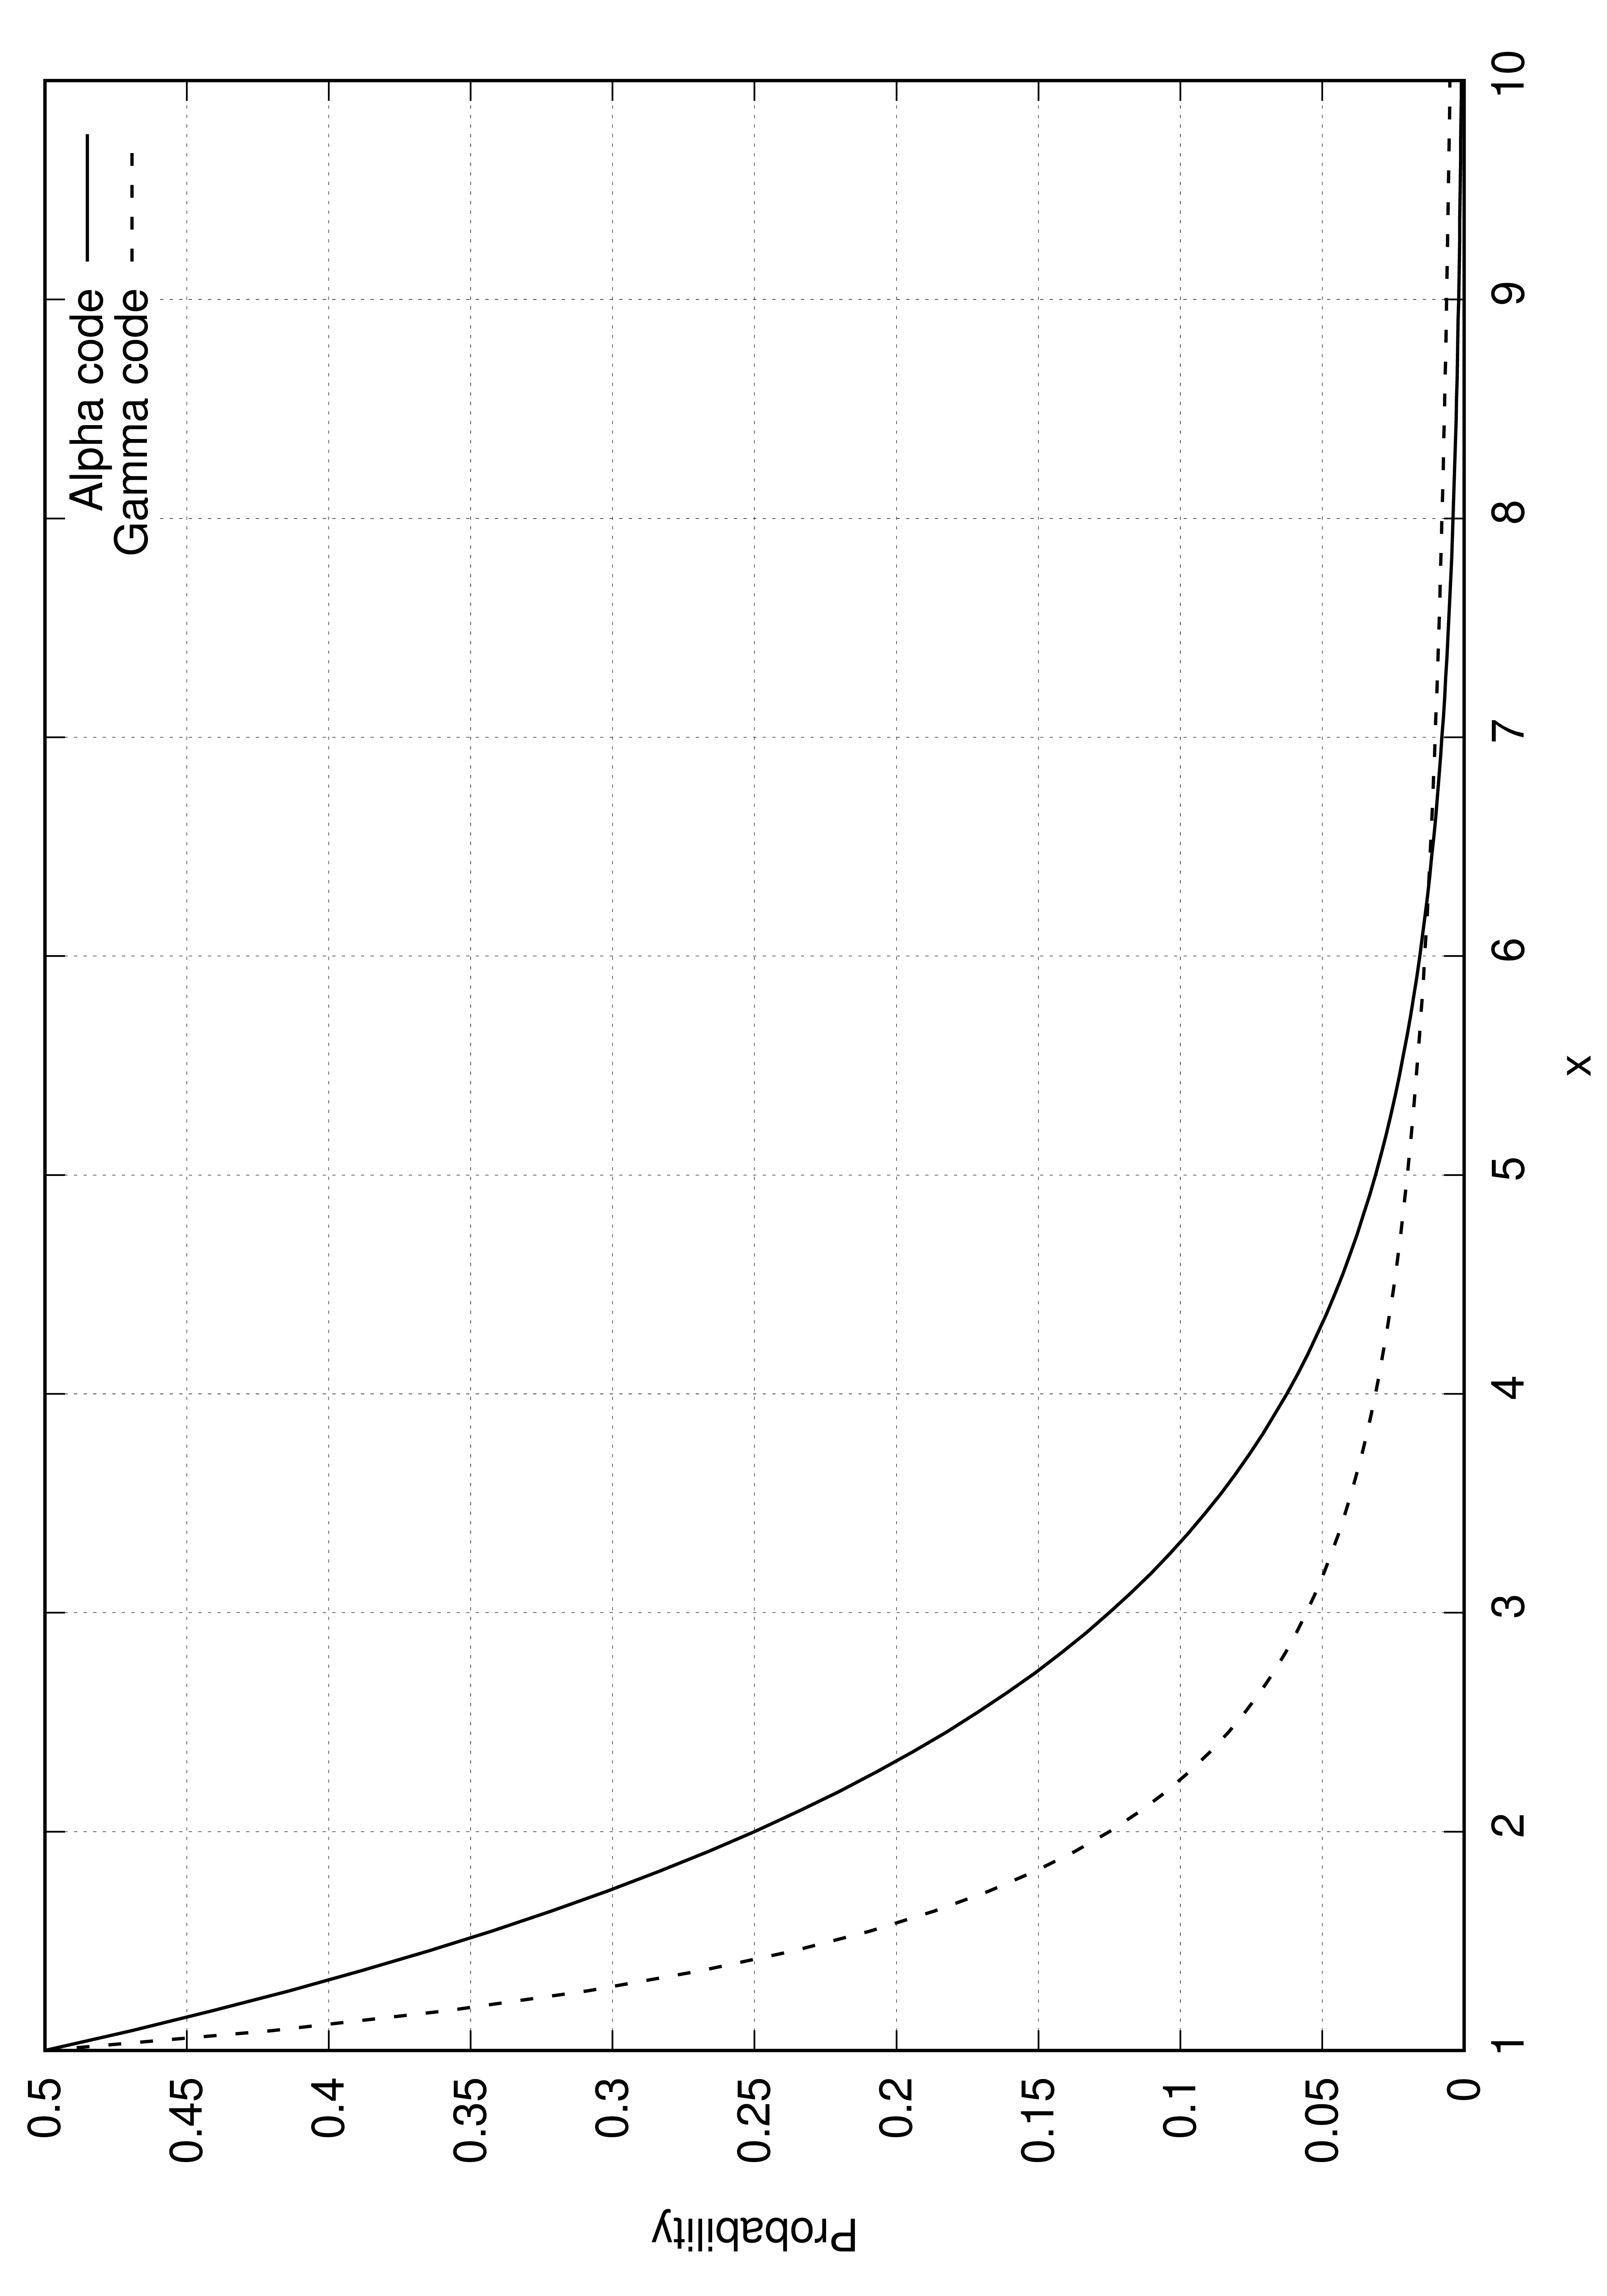
\includegraphics[width=70mm,angle=-90]{./figs/alpha_gamma_code_dist.png}
  \end{center}
  \caption{$\alpha$符号と$\gamma$符号の確率分布} \label{alpha_gamma_code_dist}
\end{figure}

これらの確率分布から読み取れる重要な性質は、符号化対象の整数値がこの確率分布に従っている場合、効率の良い圧縮が達成できる点である。図\ref{alpha_gamma_code_dist}に注目すると、$\gamma$符号は$\alpha$符号よりも分布の裾野($x$が大きい時の値)が大きく、$\alpha$符号よりも大きい整数$x$が出現しやすい記号の符号化に適していることが分かる。この様に、応用の場面では、符号化対象のデータの偏りに合わせて適切な符号を選択することが重要になる。

\subsubsection{Golomb(ゴロム)符号}

ロスレス音声コーデックで最もよく使われる符号が\textbf{Golomb(ゴロム)符号}\index{ごろむふごう@Golomb符号}である。Golomb符号は符号化パラメータ$m$を持ち、$m$により出力する符号が異なる。特に、$m$が2の冪数$m=2,4,8,16,\dots$のときのGolomb符号を\textbf{Rice(ライス)符号}\index{らいすふごう@Rice符号}と呼ぶ。各種パラメータを設定したときのGolomb符号の出力符号を表\ref{golomb_rice_code}に示す。
\begin{table}[htbp]
  \begin{center}
    \caption{各種符号パラメータ$m$を使用したときのGolomb符号} \label{golomb_rice_code}
    \begin{tabular}{c|l|l|l|l}
       整数値   & $m=2$        & $m=3$      & $m=4$     & $m=5$     \\ \hline
       $0$      & $10$         & $10$       & $100$     & $100$     \\
       $1$      & $11$         & $110$      & $101$     & $101$     \\
       $2$      & $010$        & $111$      & $110$     & $110$     \\
       $3$      & $011$        & $010$      & $111$     & $1110$    \\
       $4$      & $0010$       & $0110$     & $0100$    & $1111$    \\
       $5$      & $0011$       & $0111$     & $0101$    & $0100$    \\
       $6$      & $00010$      & $0010$     & $0110$    & $0101$    \\
       $7$      & $00011$      & $00110$    & $0111$    & $0110$    \\
       $8$      & $000010$     & $00111$    & $00100$   & $01110$   \\
       $9$      & $000011$     & $00010$    & $00101$   & $01111$   \\
      $10$      & $0000010$    & $000110$   & $00110$   & $00100$   \\
      $11$      & $0000011$    & $000111$   & $00111$   & $00101$   \\
      $12$      & $00000010$   & $000010$   & $000100$  & $00110$   \\
      $13$      & $00000011$   & $0000110$  & $000101$  & $001110$  \\
      $14$      & $000000010$  & $0000111$  & $000110$  & $001111$  \\
      $15$      & $000000011$  & $0000010$  & $000111$  & $001100$  \\
      $16$      & $0000000010$ & $00000110$ & $0000100$ & $001101$  \\
    \end{tabular}
  \end{center}
\end{table}
   
表\ref{golomb_rice_code}を見ると、整数値が大きくなるにつれて符号長は長くなるが、パラメータ$m$によってその符号長の伸びを制御している事が分かる。具体的な符号化アルゴリズムは次のように表せる。
\begin{itembox}[l]{Golomb符号化} \label{golomb_rice_algorithm}
  \begin{enumerate}
    \item 整数$x$を$m$で割った時の商を$q=\lfloor \frac{x}{m} \rfloor$、剰余を$r$とする。
    \item $q+1$を$\alpha$符号化する。
    \item $r$を以下の手順で符号化する。
      \begin{enumerate}
        \item $\log_{2} m$が整数($\iff$$m$が2の冪数)の場合は、$\log_{2} m$ bitで$r$の2進数表記した符号を出力する。
        \item $\log_{2} m$が整数ではない場合は、$b=\lceil \log_{2} m \rceil$として、更に以下の手順に従う。
          \begin{enumerate}
            \item $r < 2^{b} - m - 1$であれば、$b-1$ bitで$r$の2進数表記した符号を出力する。
            \item $r \geq 2^{b} - m - 1$であれば、$b$ bitで$b + 2^{b} - m$の2進数表記した符号を出力する。
          \end{enumerate}
      \end{enumerate}
  \end{enumerate}
\end{itembox}

Rice符号の場合は、$m$が2の冪数であることを用いると、剰余$r$の値による場合分けのコストがない上、$m$による除算が右シフト演算に、剰余が$m-1$とのAND演算によって実現できるため、高速な実装が実現できる。

Golomb符号のアルゴリズムを概観すると、Golomb符号はパラメータ$m$による商$q$と剰余$r$に分けて符号化している事が分かる。これを直感的な図にしてみると図\ref{golomb_code_explanation}のようになる。
\begin{figure}[htbp]
  \begin{center}
    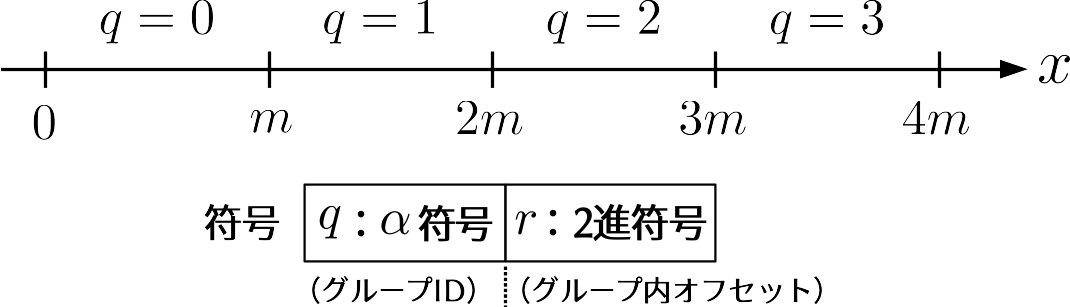
\includegraphics[width=100mm]{./figs/golomb_code_explanation.png}
  \end{center}
  \caption{Golomb符号の直感的な説明図} \label{golomb_code_explanation}
\end{figure}

整数の数直線を長さ$m$の区間で区切り、商$q$によってどの区間に入っているのかを示し、$r$によって区間内の位置を定めていると考えることができる。

Golomb符号が従う確率分布を導出する。議論の単純化のため、パラメータ$m$は2の冪乗(Rice符号)に限定する。整数$x$に対するGolomb符号の長さ$l_{G}(x)$は、商部分の$\alpha$符号は長さは$q+1$、剰余部分は長さ$\log_{2} m$だから、
\begin{eqnarray*}
  l_{G}(x) = q + 1 + \log_{2} m = \left\lfloor \frac{x}{m} \right\rfloor + 1 + \log_{2} m
\end{eqnarray*}

よって、Golomb符号が従う分布$P_{G}(x)$は、
\begin{eqnarray*}
  P_{G}(x) &=& 2^{-l_{G}(x)} = 2^{-\left( \lfloor \frac{x}{m} \rfloor + 1 + \log_{2} m \right)} = \frac{1}{2m} 2^{-\lfloor \frac{x}{m} \rfloor} \nonumber \\
  &\approx& \frac{1}{2m} 2^{-\frac{x}{m}}
\end{eqnarray*}

となる。$P_{G}(x)$が確率分布となるためには、全確率$\int^{\infty}_{0} P_{G}(x) \textrm{d}x$が$1$となる必要がある。実際に$\int^{\infty}_{0} P_{G}(x) \textrm{d}x$は、
\begin{eqnarray*}
  \int^{\infty}_{0} P_{G}(x) \textrm{d}x &=& \frac{1}{2m} \int^{\infty}_{0} 2^{-\frac{x}{m}} \textrm{d}x = \frac{1}{2m} \left[ -m \frac{2^{-\frac{x}{m}}}{\log 2} \right]^{\infty}_{0} \\
  &=& -\frac{1}{2} \left( 0 - \frac{1}{\log 2} \right) = \frac{1}{2 \log 2}
\end{eqnarray*}

この結果により、$P_{G}(x)$を$\frac{1}{2 \log 2}$で割ることで$P_{G}(x)$が確率分布となる。その結果を改めて$P_{G}(x)$と表すと、
\begin{eqnarray*}
  P_{G}(x) = \left( \frac{1}{2 \log 2} \right)^{-1} \frac{1}{2m} 2^{-\frac{x}{m}} = \frac{\log 2}{m} 2^{-\frac{x}{m}}
\end{eqnarray*}

ここで、$\lambda = \frac{\log 2}{m}$とおいて整理すると、
\begin{eqnarray}
  P_{G}(x) &=& \lambda 2^{-\frac{\lambda x}{\log 2}} \nonumber \\
  \implies \log P_{G}(x) &=& \log \lambda - \frac{\lambda x}{\log 2} \log 2 = \log \lambda - \lambda x \nonumber \\
  \implies P_{G}(x) &=& \exp \left( \log \lambda - \lambda x \right) \nonumber \\
  &=& \lambda \exp(- \lambda x) \label{golomb_code_is_exp_distribution}
\end{eqnarray}

式\ref{golomb_code_is_exp_distribution}はパラメータ$\lambda$を持つ\textbf{指数分布}に他ならない。符号化対象の整数$x$は常に離散値を取っているが、確率変数が離散値を取る場合の指数分布は\textbf{幾何分布}をなす。幾何分布は$0 < \rho < 1$を満たすパラメータ$\rho$を用いて、式\ref{golomb_code_is_geometric_distribution}で表せる。
\begin{eqnarray}
  P_{G}(x) = \rho^{x} (1 - \rho) \label{golomb_code_is_geometric_distribution}
\end{eqnarray}

幾何分布はある事象が成功する(あるいは、失敗する)までに必要とする試行回数の確率分布である。パラメータ$\rho$は試行一回あたりの失敗(あるいは、成功)確率を示している。様々なパラメータ$\rho$の値に対応する幾何分布の確率分布関数を図\ref{golomb_code_dist}に示す。
\begin{figure}[htbp]
  \begin{center}
    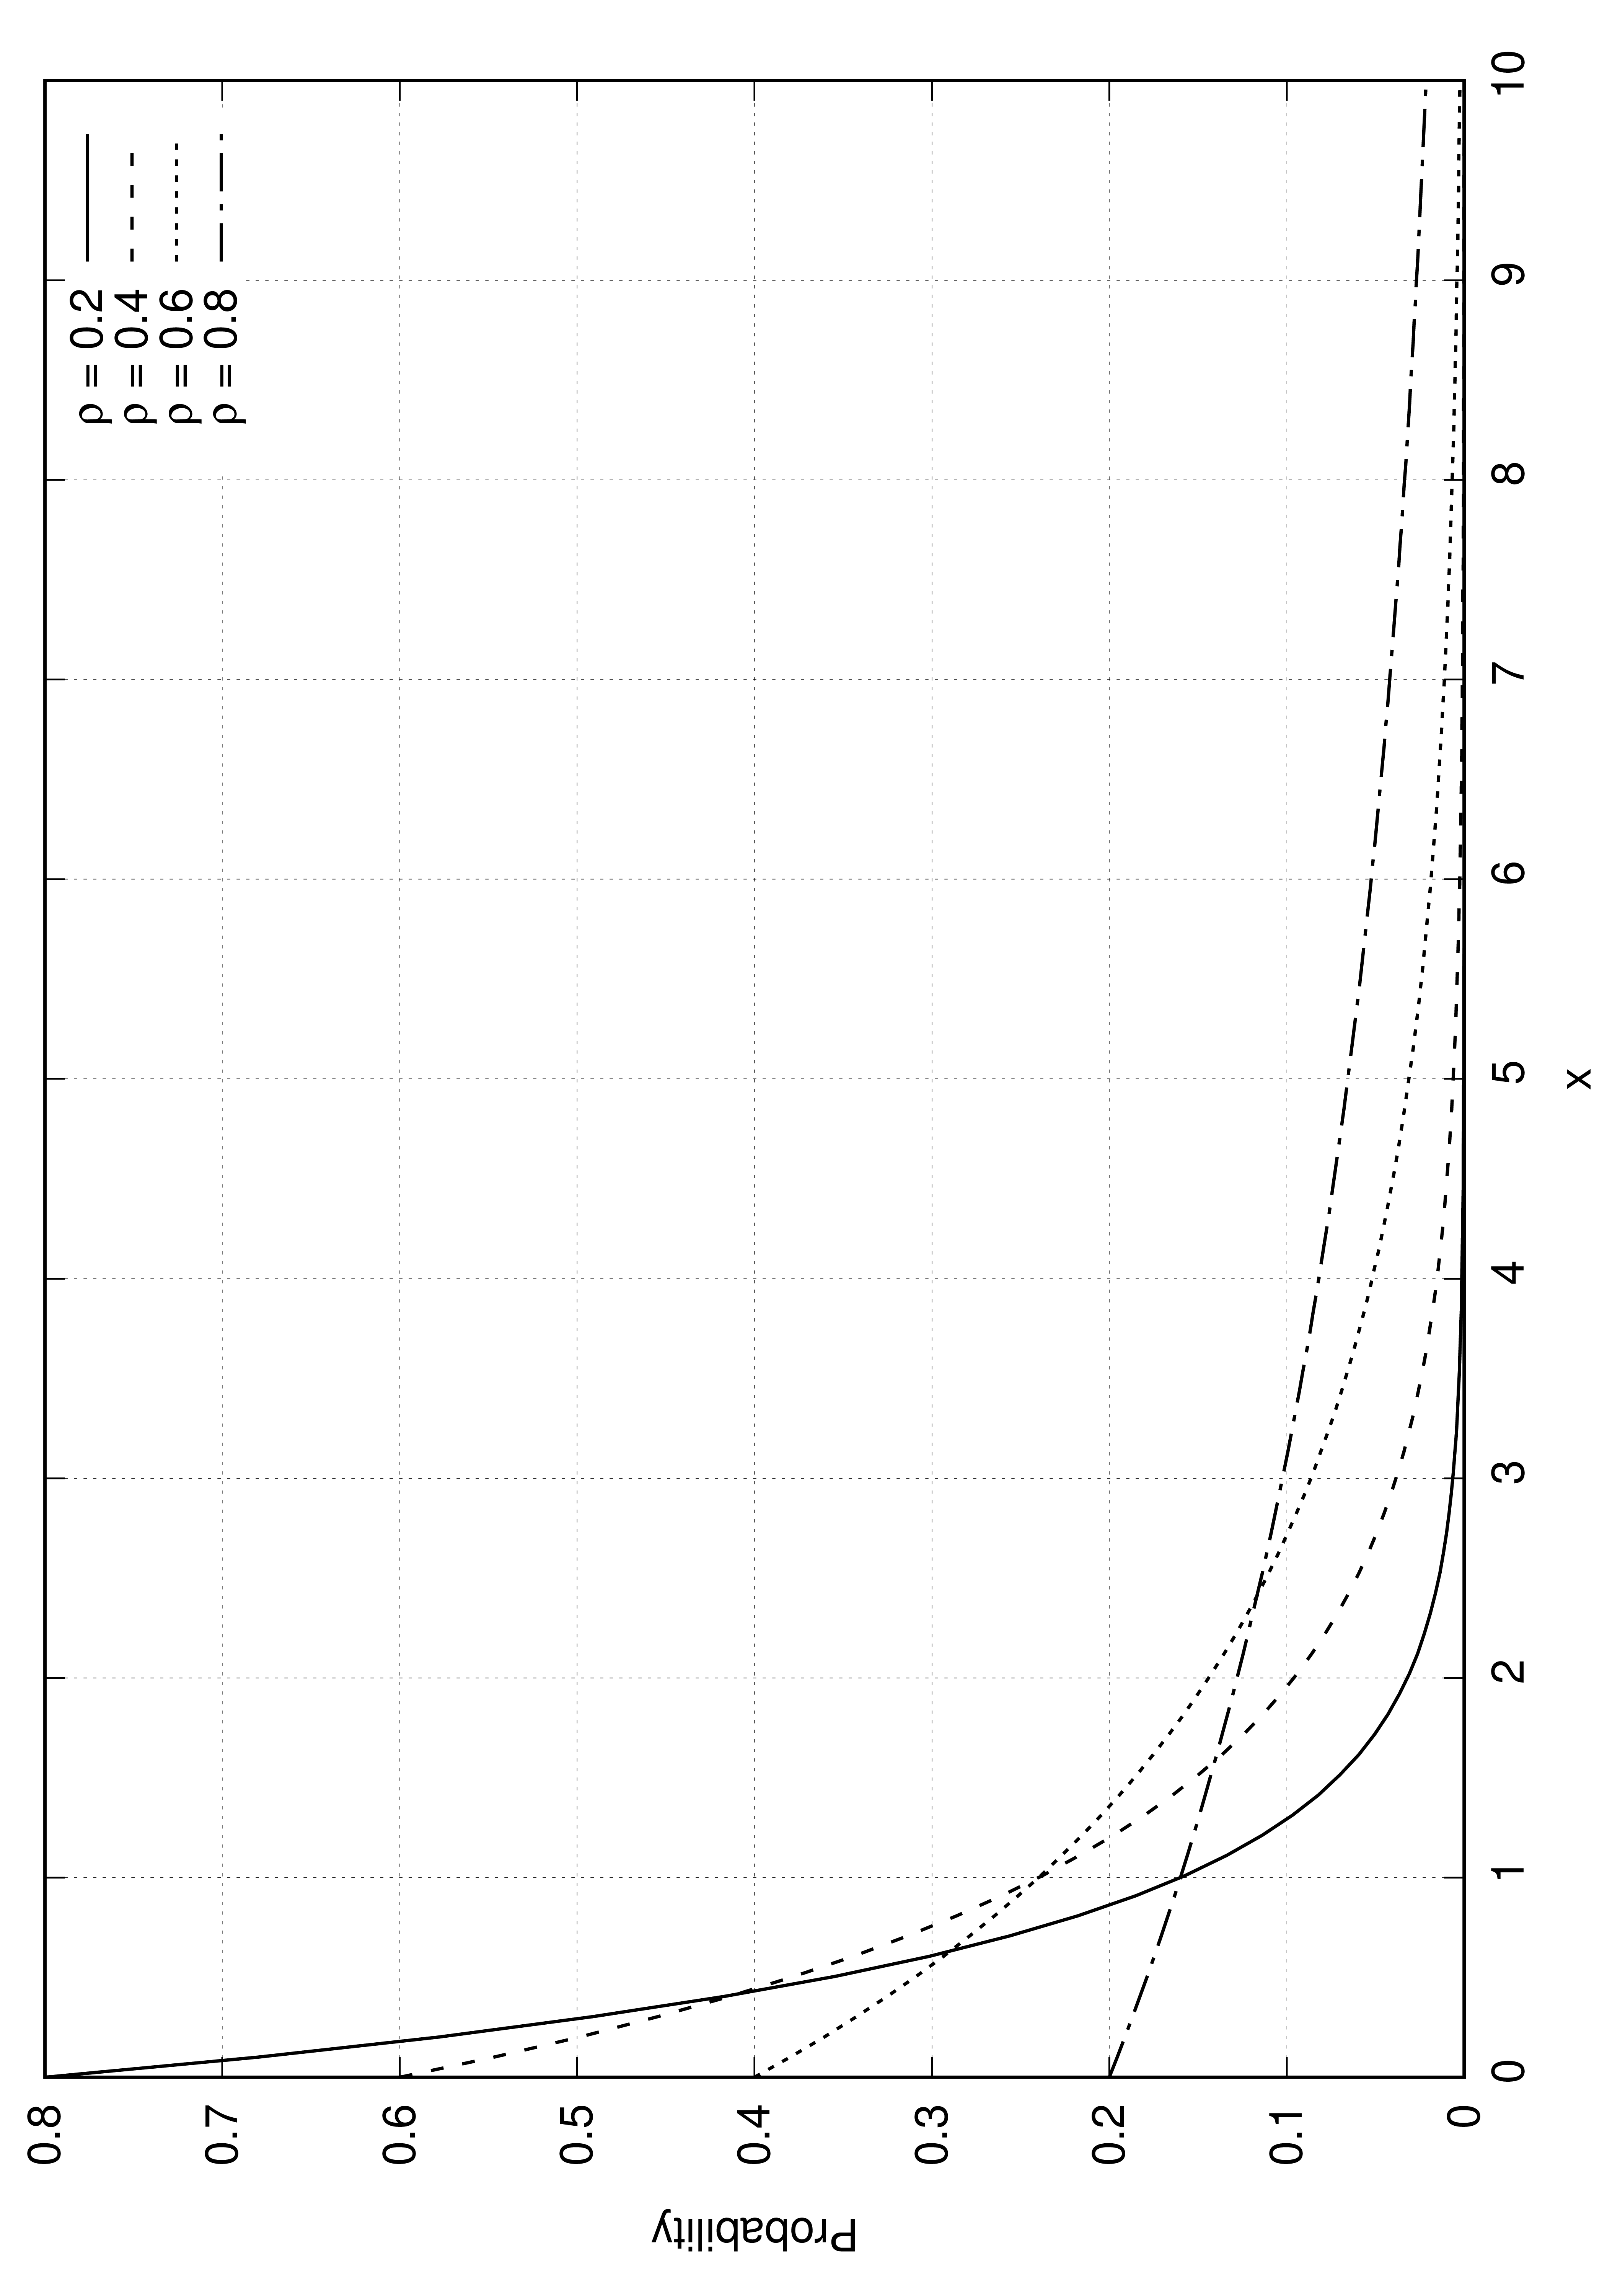
\includegraphics[width=70mm, angle=-90]{./figs/geometric_dist.png}
  \end{center}
  \caption{幾何分布(Golomb符号が従う分布$P_{G}(x)$)の確率分布} \label{golomb_code_dist}
\end{figure}

以上の議論により、Golomb符号は符号化対象のデータが幾何分布に従っているときに効率的に圧縮できることが分かる。
Golomb符号がマルチメディアのデータ圧縮に使用される主な理由として、予測による残差の分布は幾何分布に近い形を取るという経験的事実と、ハフマン符号等で必要になるテーブルといった、符号化のための追加記憶領域を必要としない点が挙げられる。

\subsubsection{Golomb(ゴロム)符号のパラメータ設定}

前節で導入したGolomb符号にはパラメータ$m$が伴っている。$m$によって効率的に符号化できる整数の分布が変わってしまうため、パラメータの調整を行うことが実用上重要になる。ここでは、\cite{optimalgolombparam}に記載のある、JPEG2000で採用されている手法に従って最適なパラメータの導出を行う。

手法の鍵となるアイデアは、観測した整数$x$の平均$\mathrm{E}[x]$に合わせて$m$を上手く選ぶことで、$P_{G}(x)$の分布を$\alpha$符号の持つ分布に近づける事である。

まず、幾何分布の定義式\ref{golomb_code_is_geometric_distribution}に従って平均$\textrm{E}[x]$を求めると、
\begin{eqnarray}
  \mathrm{E}[x] &=& \sum_{x=0}^{\infty} x P_{G}(x) = \sum_{x=0}^{\infty} x(1-\rho)\rho^{x} \nonumber \\
  &=& (1 - \rho) \sum_{x=0}^{\infty} x \rho^{x} = (1 - \rho) \frac{\rho}{(1 - \rho)^{2}} \nonumber \\
  &=& \frac{\rho}{1 - \rho} \label{mean_and_rho}
\end{eqnarray}

となり\footnote{ここで、$\sum_{x=0}^{\infty} x \rho^{x} = \frac{\rho}{(1-\rho)^{2}}$を用いている。証明は、等比級数の和$\sum_{x=0}^{\infty} \rho^{x} = \frac{1}{1-\rho}$の両辺を$\rho$で微分すると$\sum_{x = 0}^{\infty} x \rho^{x - 1} = \frac{1}{(1 - \rho)^{2}}$となり、この両辺に$\rho$を乗ずることで欲しい式が得られる。}、パラメータ$\rho$から平均$\textrm{E}[x]$が求まることが分かる。

次に$P_{G}(x)$の分布を$\alpha$符号に近づける事を考えるが、式\ref{golomb_code_is_geometric_distribution}のままではパラメータ$m$が陽に現れないため、議論が進まない。そこで、幾何分布の整数を$m$個毎にまとめ、商$q$についての確率分布$P_{G_{m}}(q)$を以下の式で定義する。
\begin{eqnarray}
  P_{G_{m}}(q) = \sum_{r=0}^{m-1} P_{G}(qm + r) \label{grouped_golomb_distribution_definition}
\end{eqnarray}

式\ref{grouped_golomb_distribution_definition}に式\ref{golomb_code_is_geometric_distribution}を代入すると、
\begin{eqnarray}
  P_{G_{m}}(q) &=& \sum_{r=0}^{m-1} P_{G}(qm + r) = \sum_{r=0}^{m-1} \rho^{qm+r}(1 - \rho) \nonumber \\
  &=& (1 - \rho) \rho^{qm} \sum_{r=0}^{m-1} \rho^{r} \nonumber \\
  &=& (1 - \rho) \rho^{qm} \frac{1 - \rho^{m}}{1 - \rho} \quad (\because 等比級数の和の公式) \nonumber \\
  &=& \rho^{qm} (1 - \rho^{m}) \label{grouped_golomb_distribution}
\end{eqnarray}

が得られる。この式\ref{grouped_golomb_distribution}において、$\rho^{m} = \frac{1}{2}$であれば、$P_{G_{m}}(q) = (\frac{1}{2})^{q} \times \frac{1}{2} = 2^{-q-1}$となって確率分布が$\alpha$符号に一致し、理想的な符号化が行える。現実の残差は$0$に偏って出現することは稀という仮定\footnote{この仮定から、ほぼ無音の音声に対して圧縮率が悪くなる。}から、図\ref{golomb_code_dist}から観察できるように$\rho \approx 1$とすると、$\rho^{m}$は次のように近似できる。
\begin{eqnarray}
  \rho^{m} &=& \left\{ 1 - (1 - \rho) \right\}^{m} \approx 1 - m(1-\rho) \nonumber \\
  &\approx& 1 - m \frac{1 - \rho}{\rho} \nonumber \\
  &=& 1 - \frac{m}{\textrm{E}[x]} \quad (\because 式\ref{mean_and_rho}を使用) \label{approx_of_rho_m}
\end{eqnarray}

$\rho^{m}$の近似式\ref{approx_of_rho_m}に$\rho^{m} = \frac{1}{2}$の条件を入れることで、$m$についての式を得る。
\begin{eqnarray}
  \rho^{m} &\approx& 1 - \frac{m}{\textrm{E}[x]} = \frac{1}{2} \nonumber \\
  \implies m &=& \frac{\textrm{E}[x]}{2} \label{optimal_golomb_parameter}
\end{eqnarray}

式\ref{optimal_golomb_parameter}が最適なパラメータ$m$を求める式の一つである。JPEG2000においては、高速化のためRice符号のパラメータ$k$を$m = 2^{k}$として、式\ref{optimal_golomb_parameter}の両辺の$\log_{2}$を取り、以下の式\ref{optimal_rice_parameter}で最適なパラメータ$k$を設定する。
\begin{eqnarray}
  k = \max \left\{ 0, \left\lceil \log_{2} \left( \frac{\textrm{E}[x]}{2} \right) \right \rceil \right\} \label{optimal_rice_parameter}
\end{eqnarray}

$\textrm{E}[x]$は推定値で置き換えても良いため、観測した整数の移動平均等から適応的にパラメータ$m,k$を求めることができる。

\chapter{実装編} 

基本理論をベースに、筆者はロスレス音声コーデック\texttt{ALA}を扱うコマンドラインツール(以下、\texttt{ALA}コマンドラインツールと呼ぶ)をC言語フルスクラッチで作成した。
本ツールは、\texttt{wav}ファイルのエンコードと、エンコード済みバイナリファイルを\texttt{wav}ファイルにデコードする機能を持つ。

ソースファイルは\texttt{github}にアップしている。以下のURLを参照のこと。
\begin{itemize}
  \item \url{https://github.com/MrAiki/ALA}
\end{itemize}

\texttt{ALA}は以下のソースファイルから構成され、それぞれ以下の役割を持つ。
\begin{description}
  \item[\texttt{main.c}] メインエントリ(\texttt{main}関数)
  \item[\texttt{ala\char`_predictor.c, ala\char`_predictor.h}] 予測/合成モジュール
  \item[\texttt{ala\char`_coder.c, ala\char`_coder.h}] 符号化/復号モジュール
  \item[\texttt{ala\char`_utility.c, ala\char`_utility.h}] 計算時ユーティリティ
  \item[\texttt{bit\char`_stream.c, bit\char`_stream.h}] bit単位の入出力モジュール
  \item[\texttt{wav.c, wav.h}] wavファイル入出力モジュール
  \item[\texttt{Makefile}] メイクファイル
\end{description}

本章では、まず\texttt{ALA}コマンドラインツールの使用方法を述べ、次に\texttt{ALA}のファイルフォーマットを解説する。続いて、各ソースファイルについて実装説明を行う。

\section{\texttt{ALA}コマンドラインツールの使用方法}

\subsection{ビルド方法}

\texttt{ALA}コマンドラインツールをビルドするには、コマンドライン上で\texttt{make}を実行する\footnote{\texttt{gcc}が必要である。Windowsでビルドする場合は、Windows Subsystem for Linuxの使用を推奨。}。
\begin{flushleft}
  \texttt{\$ make}
\end{flushleft}

\footnote{\texttt{\$}はコマンドプロンプトであり、実際には入力する必要はない。}\texttt{gcc}により各ソースがコンパイルされる。ビルドに成功すれば、成果物として実行可能形式ファイル\texttt{ala}が出力される。

\subsection{実行}
\subsubsection{エンコード} 手元のwavファイルをエンコードする際には、\texttt{ala}をビルドした上で以下のコマンドを実行する。
\begin{flushleft}
  \texttt{\$ ./ala -e 入力ファイル.wav 出力ファイル}
\end{flushleft}

エンコード処理が実行され、成功した場合は圧縮済みのバイナリファイルが出力される。
\subsubsection{デコード} エンコード済みのバイナリファイルをデコードする際は、以下のコマンドを実行する。
\begin{flushleft}
  \texttt{\$ ./ala -d 入力ファイル 出力ファイル.wav}
\end{flushleft}
デコード処理により\texttt{wav}ファイルが復元される。

\section{\texttt{ALA}ファイルフォーマット}

\texttt{ALA}コマンドラインツールでエンコードしたファイル(以下、\texttt{ALA}ファイルと呼ぶ)の構成概要図を図\ref{ala_file_format}に示す。
\begin{figure}[htbp]
  \begin{center}
    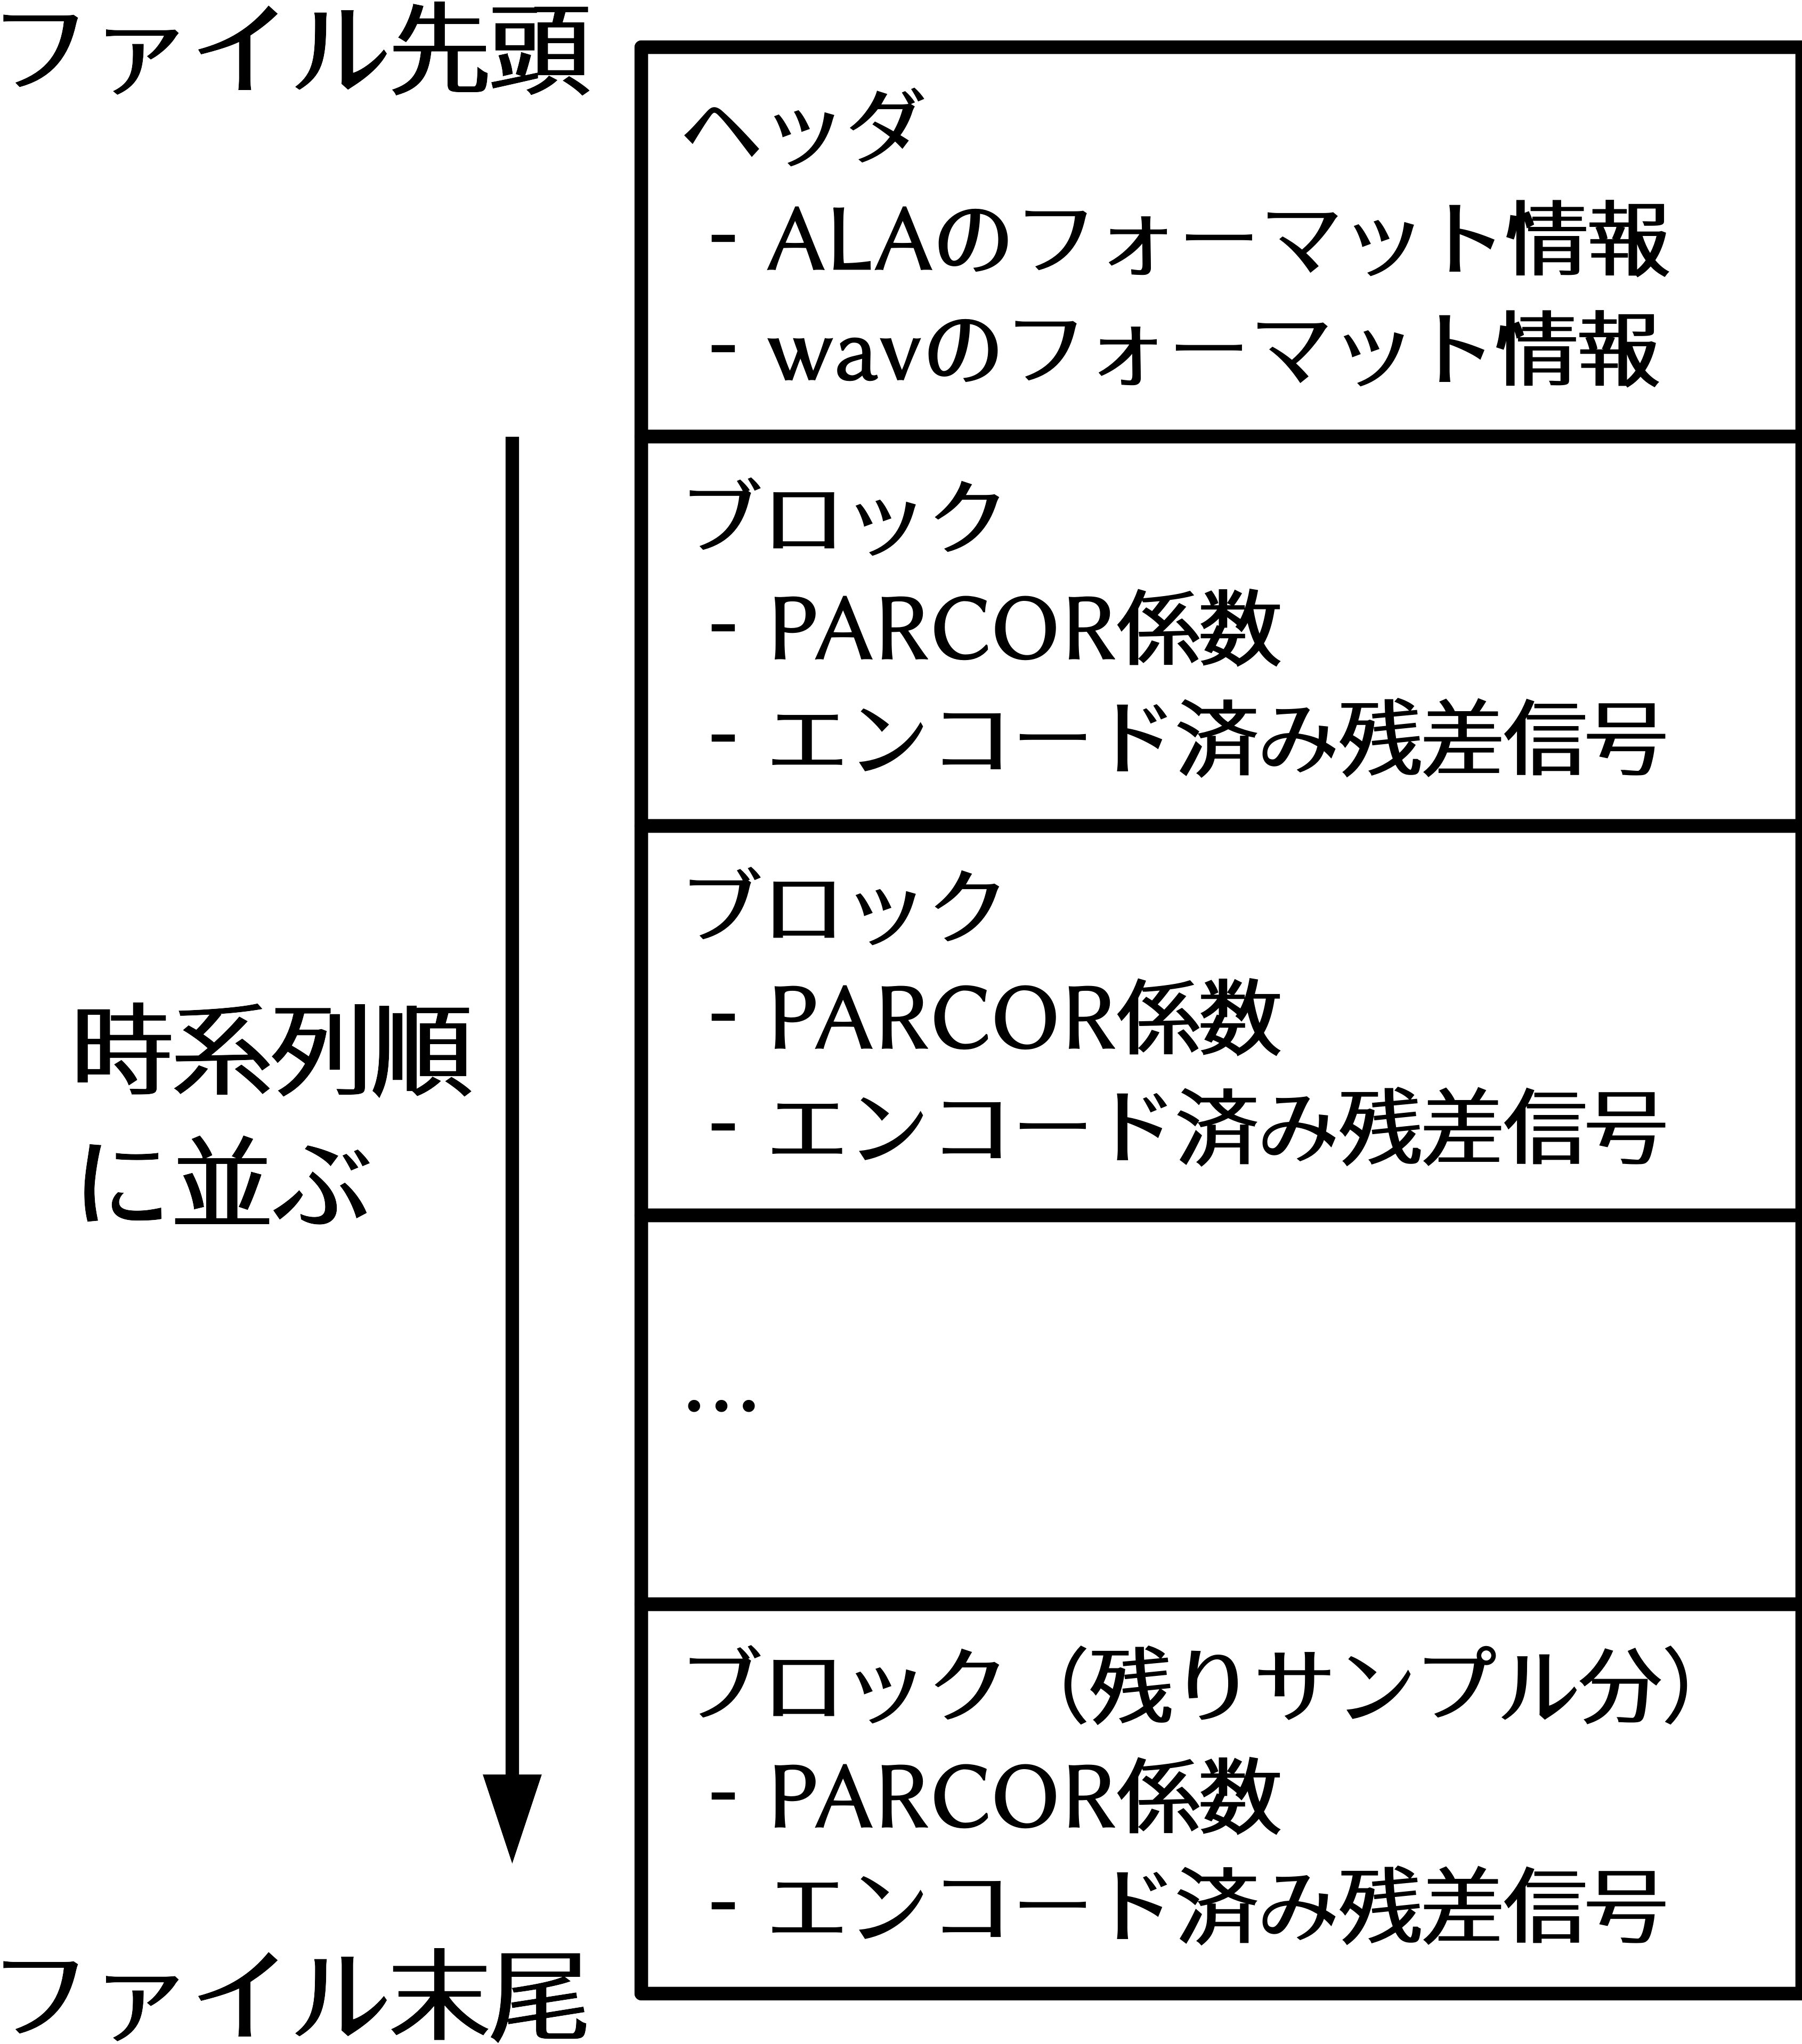
\includegraphics[width=60mm]{./figs/ala_file_format.png} 
    \caption{\texttt{ALA}ファイルの構成概要} \label{ala_file_format}
  \end{center}
\end{figure}

\texttt{ALA}ファイルの先頭には、\texttt{ALA}のフォーマット情報やエンコードしたwavのフォーマット情報を含む\textbf{ヘッダ}が記録されている。ヘッダに続き、一定サンプル数単位で波形データを符号化した\textbf{ブロック}がエンコードした波形の時系列順に並んでいる。

本節では\texttt{ALA}のヘッダとブロックのフォーマットを紹介する。なお、\texttt{ALA}はバイナリデータを全て\textbf{ビッグエンディアン}で記録している。

\subsection{ファイルヘッダフォーマット}

表\ref{ala_header_format}に、\texttt{ALA}ファイルのヘッダフォーマットを示す。
\begin{table}[htbp]
  \begin{center}
    \caption{\texttt{ALA}のヘッダフォーマット} \label{ala_header_format}
    \begin{tabular}{|c|l|l|}
      \hline
      bit幅 & 内容 & 補足                         \\ \hline
      32 & \texttt{'A', 'L', 'A', '\char`\\0'}  & \texttt{ALA}ファイルであることを示すシグネチャ   \\ \hline
      16 & フォーマットバージョン               & バイナリフォーマットのバージョン                 \\ \hline
       8 & チャンネル数                         &                                                  \\ \hline
      32 & サンプル数                           & 1チャンネルあたりのサンプル数を示す              \\ \hline
      32 & サンプリングレート                   &                                                  \\ \hline
       8 & サンプルあたりbit数                  &                                                  \\ \hline
      16 & ブロックあたりサンプル数             & ファイル末尾ではこの数値より小さくなるので注意   \\ \hline
       8 & PARCOR係数次数                       & 全ブロックで同一の次数を用いる                   \\ \hline
    \end{tabular}
  \end{center}
\end{table}

\texttt{ALA}では実装の簡略化のため、末尾を除くブロックのサンプル数と、PARCOR係数の次数を同一にしている。一般に圧縮率を高めるには、波形の特性に合わせてブロックサイズやPARCOR係数(線形予測係数)の次数を可変にする\cite{mpeg4als, tak}方策が取られる。

\subsection{ブロックフォーマット}

表\ref{ala_block_format}に、\texttt{ALA}ファイルのブロックフォーマットを示す。
\begin{table}[htbp]
  \begin{center}
    \caption{\texttt{ALA}のブロックフォーマット} \label{ala_block_format}
    \begin{tabular}{|c|l|l|}
      \hline
      bit幅 & 内容 & 補足                                                                  \\ \hline
      16   & \texttt{0xFFFF}            & ブロック先頭を示す同期コード                     \\ \hline
      $x$  & PARCOR係数                 & 
      \begin{tabular}{l}
        $x = 16 \times \textrm{PARCOR}係数次数 \times 波形チャンネル数$ \\
        1チャンネル目係数列、 2チャンネル目係数列、 ... \\ の順序で記録
      \end{tabular} \\ \hline
      不定 & エンコード済みの残差 & 
      \begin{tabular}{l}
        1チャンネル目残差、 2チャンネル目残差、 ... \\ の順序で記録
      \end{tabular} \\ \hline
    \end{tabular}
  \end{center}
\end{table}

ブロック先頭の同期コードは、デコード時に現在読み出している位置が正しいかどうかを判定する目的で使用する。しかし、この同期コードはおまじない程度にしか効果がない。PARCOR係数や、エンコード済みの残差のbit列の中に\texttt{0xFFFF}が表れた場合、その場所をブロック先頭と誤判定する可能性がある。より厳格な対策として、ブロックデータのチェックサム値や巡回冗長検査(CRC16、CRC32等)の計算結果をブロックに記録しておき、デコード時に検査する対策がとられる\cite{flac,tak,mpeg4als,tta}。\texttt{ALA}では実装の簡略化のため、シグネチャと同期コード以外にデータの正しさをチェックする機能を省いている。

\section{\texttt{ala\char`_predictor.c}}

\texttt{ala\char`_predictor.c}には、予測と合成処理を行う関数群が集められている。
\begin{itemize}
  \item PARCOR係数計算
  \item PARCOR予測/合成フィルター
  \item プリエンファシス/デエンファシス
  \item チャンネル間相関除去(MS処理)
\end{itemize}

本節では、これらの計算処理について説明する。計算処理は全て\textbf{固定小数演算}により実現されているため、コードの説明の前置きとして固定小数演算についての補足説明を入れる。また、プリエンファシス/デエンファシスと、チャンネル間相関除去については基本理論で触れていない為、本節で簡易に補足を入れる。なお、PARCOR係数計算については、リスト\ref{lpc_example}(\ref{lpc_example_impl}節)で既に取り上げているため説明を省略する。

\subsection{固定小数演算}

\textbf{固定小数(fixed-point float)}\index{こていしょうすう@固定小数}とは、小数点が固定されたbit位置にある小数の表現法である。一方、C言語で\texttt{float, double}等の型を持つ浮動小数点数は、指数部の値により小数点が移動する。固定小数点は整数によって表すことができ、また、固定小数同士の演算も整数演算によって実行できる。ここでは、\cite{fixedfloat, hdlabfixedfloat}を参考にしながら固定小数演算についての解説を行う。

固定小数を用いる理由は主に2点ある。1つは、浮動小数演算を用いるとCPUやFPUの差異により計算結果が異なる場合がある。例えば、微小な数値を扱う際に、丸めの方向が異なったり、桁落ちが発生した時の動作が異なる\cite{msfloat}。この特性があると、エンコードした時の演算結果とデコードした時の演算結果に差異が発生し、ビットパーフェクトに復元できなくなる可能性がある。一方、整数演算は、同一の整数型で同一の演算を行えば結果を復元することが可能である。固定小数を用いるもう1つの理由は、整数演算を備えているプラットフォームは多く存在しているため、移植がしやすいという点が挙げられる。

\subsubsection{固定小数による小数の表記}

簡単な例として、下位4bitを小数部、上位4bitを整数部とした8bit固定小数を考えてみる。この固定小数における小数の表示例を表\ref{fixedfloat8x8}に示す。なお、整数部の上位1bitは符号bitとして、2の補数表現により負数を表現する。
\begin{table}[htbp]
  \begin{center}
    \caption{下位4bitを小数部、上位4bitを整数部とした8bit固定小数の数値例} \label{fixedfloat8x8}
    \begin{tabular}{|l|c||l|c|}
      \hline
      10進小数 & 8bit固定小数(2進数)& 10進小数  & 8bit固定小数(2進数) \\ \hline
      $7.9375$ & 0111 1111            & $-0.0625$ & 1111 1111             \\ \hline
      $7.875$  & 0111 1110            & $-0.125$  & 1111 1110             \\ \hline
      $7.8125$ & 0111 1101            & $-0.1875$ & 1111 1101             \\ \hline
      $7.75$   & 0111 1100            & $-0.25$   & 1111 1100             \\ \hline
      $\vdots$ & $\vdots$             & $\vdots$  & $\vdots$              \\ \hline
      $0.1875$ & 0000 0011            & $-7.8125$ & 1000 0011             \\ \hline
      $0.125$  & 0000 0010            & $-7.875$  & 1000 0010             \\ \hline
      $0.0625$ & 0000 0001            & $-7.9375$ & 1000 0001             \\ \hline
      $0.0$    & 0000 0000            & $-8.0$    & 1000 0000             \\ \hline
    \end{tabular}
  \end{center}
\end{table}

表\ref{fixedfloat8x8}の観察から、固定小数は符号付き整数と全く同様の順序関係を持っていることが分かる。また、最大値$7.9375$は最小値$-8.0$よりも絶対値が小さいことや、正数よりも負数の方が多い性質を持つ。

一般に小数部に$n$bit使用した際に、整数で表現された固定小数$f$は以下の式\ref{fixedtodesimal}で10進小数$d$に変換できる。
\begin{eqnarray}
  d = f \times 2^{-n} \label{fixedtodesimal}
\end{eqnarray}

逆に、10進小数$d$は以下の式\ref{desimaltofixed}で固定小数$f$に変換できる。
\begin{eqnarray}
  f = \textrm{round}(d \times 2^{n}) \label{desimaltofixed}
\end{eqnarray}

ここで$\textrm{round}$は整数への丸めを行う関数である\footnote{丸めは一意に定まらない。最も近い整数に丸めることもあれば、無条件に切り捨て/切り上げを行う操作を差して丸めと言う場合もある。}。式\ref{fixedtodesimal}, \ref{desimaltofixed}で現れる2の冪乗数による乗算は、C言語では$n$bitのシフト演算により変換を行うことができる。

\subsubsection{固定小数演算}

固定小数どうしの加算と減算は、整数の加算と減算と全く同様に計算できる。$n$bitの小数部を持つ固定小数$f_{1}, f_{2}$に対応する10進小数を$d_{1}, d_{2}$で表すと、加算$d_{1} + d_{2}$と減算$d_{1} - d_{2}$は式\ref{fixedtodesimal}により、
\begin{eqnarray*}
  d_{1} + d_{2} &=& f_{1} \times 2^{-n} + f_{2} \times 2^{-n} = (f_{1} + f_{2}) \times 2^{-n} \\
  d_{1} - d_{2} &=& f_{1} \times 2^{-n} - f_{2} \times 2^{-n} = (f_{1} - f_{2}) \times 2^{-n}
\end{eqnarray*}

となるため、整数加算と減算をそのまま行えば良い。

固定小数どうしの乗算は、整数乗算を行う際に小数部bit分だけ右シフトを行う必要がある。何故なら、式\ref{fixedtodesimal}を用いて乗算$d_{1} \times d_{2}$を計算してみると、
\begin{eqnarray*}
  d_{1} \times d_{2} &=& f_{1} \times 2^{-n} \times f_{2} \times 2^{-n} \\
  &=& (f_{1} \times f_{2} \times 2^{-n}) \times 2^{-n}
\end{eqnarray*}

となる。固定小数どうしの乗算を行うことで、$f_{1} \times f_{2} \times 2^{-n}$の結果は得られるが、最後の$2^{-n}$の乗算が不足している事が分かる。この為、整数乗算結果に対して$2^{-n}$を乗ずる(C言語では$n$bitの算術右シフトを行う)ことが必要である\footnote{固定小数に対して$2^{-n}$を乗ずるタイミングは、乗算前でも良い。}。

乗算の計算例を挙げる。表\ref{fixedfloat8x8}を参考に、$7.75 \times -0.25$を考えてみる。$7.75$に対応する整数値は$01111100 = 124$、$-0.25$に対応する整数値は$11111100 = -4$である。整数乗算の結果$124 \times -4 = -496$が得られ、これに$2^{-4}=1/16$を乗ずることで$-31$が得られる。$-31$に$2^{-4}$を乗じて10進小数に戻すと$-1.9375$が得られ、これは$7.75 \times -0.25$の結果に一致していることが確認できる。

固定小数の乗算処理を実装する際に注意すべき点\footnote{$\iff$筆者が躓いた点}を2点挙げる。整数のオーバーフローと、右シフト時の切り捨てである。

まず、固定小数は整数部のbit幅が狭くなっているため、乗算によってオーバーフローが発生しやすい。例えば、24bitの量子化bit数を持つwavファイルを扱う際に小数部のbit数を24とすると、32bit整数型(\texttt{int32\char`_t}等)を使用した際にオーバーフローが発生するので注意が必要である。対応としては、64bit整数型(\texttt{int64\char`_t}等)を使うか、オーバーフローが発生しないように乗算前に数値を右シフトしておくことが考えられる。

もう1点の右シフト時の切り捨てについても注意すべきである。乗算後の右シフトを何も考えずに行うと、乗算結果が負に偏って表れやすくなる。何故なら、C言語の算術右シフト演算は、正整数\texttt{1}に対する1bit右シフト\texttt{1 >> 1}の結果は\texttt{0}になる一方で、負整数\texttt{-1}に対する1bit右シフト\texttt{-1 >> 1}は\texttt{-1}のままとなるからである。この現象に対しては、乗算結果に$0.5$を加えてから右シフトを行う(正の無限大方向に切り上げる)ことで偏りをある程度緩和できる。

次に固定小数どうしの除算について見ていく。除算では、乗算とは逆に小数部bit数だけ左シフトを行う必要がある。理由としては、再度$n$bitの小数部を持つ固定小数$f_{1}, f_{2}$とそれに対応する10進小数$d_{1}, d_{1}$を用いた際に、$d_{1} / d_{2}$は、
\begin{eqnarray*}
  d_{1} / d_{2} &=& (f_{1} \times 2^{-n}) / (f_{2} \times 2^{-n}) \\
  &=& (f_{1} / f_{2} \times 2^{-n}) / 2^{-n} = (f_{1} / f_{2} \times 2^{-n}) \times 2^{n}
\end{eqnarray*}

となり、$2^{n}$の乗算が追加で必要になることが分かる。\texttt{ALA}においては除算は使用していないため、立ち入った説明は行わない。

\subsection{PARCOR予測フィルター}

PARCOR係数による予測は、端的に言えば格子型フィルター(図\ref{cascaded_lattice_filter_residual}、式\ref{parcor_forward_residual}、式\ref{parcor_backward_residual})をそのままコードに落とし込んだものである。式\ref{parcor_forward_residual}、式\ref{parcor_backward_residual}を再掲する。
\begin{eqnarray*}
  f_{M}(n) &=& f_{M-1}(n) - \gamma_{M} b_{M-1}(n-1) \quad (式\ref{parcor_forward_residual}を再掲) \\
  b_{M}(n) &=& b_{M-1}(n - 1) - \gamma_{M} f_{M-1}(n) \quad (式\ref{parcor_backward_residual}を再掲)
\end{eqnarray*}

また、PARCOR係数による格子型予測フィルターの図(図\ref{cascaded_lattice_filter_residual})をここに再掲する。
\begin{figure}[htbp]
  \begin{center}
    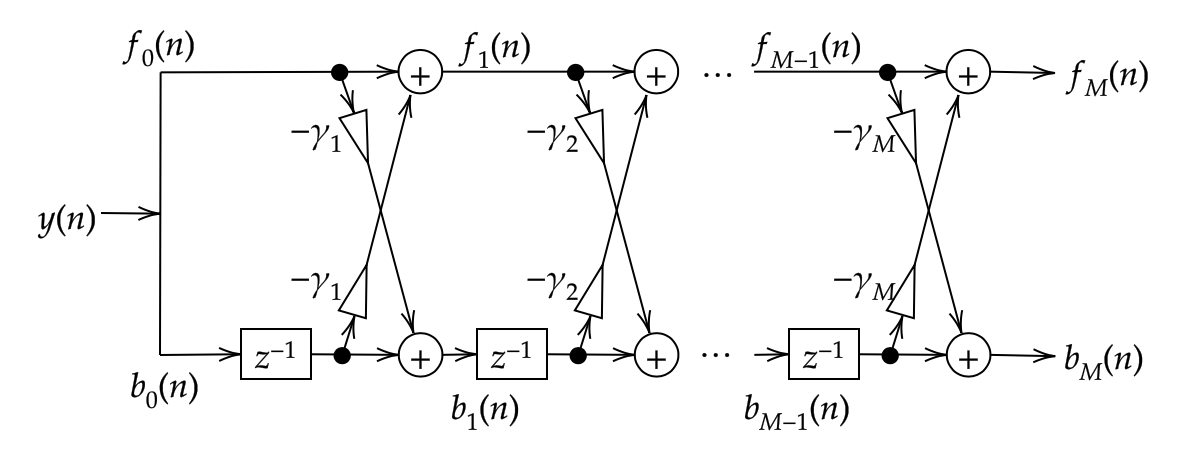
\includegraphics[width=120mm]{./figs/cascaded_lattice_filter_residual.png}
    \caption{格子型フィルターの連結(図\ref{cascaded_lattice_filter_residual}を再掲)}
  \end{center}
\end{figure}

PARCOR係数を用いた予測フィルターの実装部分をリスト\ref{parcor_predict}に示す。
\lstinputlisting[linerange={283-334,99999-999999}, firstnumber=283, caption=PARCOR予測フィルター実装(\texttt{ala\char`_predictor.c}), label=parcor_predict]{./ALA/ala_predictor.c}

固定小数演算を行うにあたり、小数部のbit幅は15としている(16bitとすると、32bit整数の乗算時にオーバーフローが発生する可能性があるため\footnote{例えば、16bit整数の最大値65535どうしの乗算は$65535 \times 65535 = 4294836225$。これは、符号付き32bit整数の最大値を超えておりオーバーフローしている。})。
このソースに対して幾つか補足を入れる。

\subsubsection{乗算時の右シフト対策の定数}

\lstinputlisting[linerange={293-294,99999-999999}, firstnumber=293, caption=乗算時の定数(\texttt{ala\char`_predictor.c}), label=fixed_half]{./ALA/ala_predictor.c}

乗算時の右シフトによる切り捨てに対策するための定数\texttt{half}を定義している。小数部のbit幅が15のため、$0.5$は1を14bit左シフトして得ることができる。

\subsubsection{前向き誤差計算}

\lstinputlisting[linerange={313-320,99999-999999}, firstnumber=313, caption=前向き誤差計算(\texttt{ala\char`_predictor.c}), label=calc_forward_residual]{./ALA/ala_predictor.c}

式\ref{parcor_forward_residual}に従って低次の前向き誤差から順次前向き計算を行っている。途中、固定小数乗算を行い変数\texttt{mul\char`_temp}に代入している。注目すべきは\texttt{ALAUTILITY\char`_SHIFT\char`_RIGHT\char`_ARITHMETIC}マクロである。これは算術右シフト演算を確実に行うためのマクロであり、\texttt{ala\char`_utility.h}に定義がある。

\lstinputlisting[linerange={11-20,99999-999999}, firstnumber=11, caption=算術右シフトマクロ(\texttt{ala\char`_utility.h}), label=arithmetic_right_shift]{./ALA/ala_utility.h}

一般に整数型に対する右シフト演算(\texttt{>>})は、算術右シフト演算になるとは限らない\cite{hackersdelight}ため、符号なし整数を用いた算術右シフト演算を定義している。

\subsubsection{後ろ向き誤差計算}

\lstinputlisting[linerange={321-328,99999-999999}, firstnumber=321, caption=後ろ向き誤差計算(\texttt{ala\char`_predictor.c}), label=calc_backward_residual]{./ALA/ala_predictor.c}

式\ref{parcor_backward_residual}に従って後ろ向き誤差を更新している。前向き誤差とは異なり、変数\texttt{backward\char`_residual[ord]}は次のループで計算で使用するために、コウジィ…から低次後ろ向き誤差に向かって更新を行わなければならない。

\subsection{PARCOR合成フィルター}

PARCOR係数による残差からの合成処理についても格子型フィルター(図\ref{cascaded_lattice_filter_synthesis}, 式\ref{parcor_forward_synthesis}, 式\ref{parcor_backward_residual})の実装を素直に行うだけである。式\ref{cascaded_lattice_filter_synthesis}、式\ref{parcor_backward_residual}を再掲する。
\begin{eqnarray*}
  f_{M-1}(n) &=& f_{M}(n) + \gamma_{M} b_{M-1}(n-1) \quad (式\ref{parcor_forward_synthesis}を再掲) \\
  b_{M}(n) &=& b_{M-1}(n - 1) - \gamma_{M} f_{M-1}(n) \quad (式\ref{parcor_backward_residual}を再掲)
\end{eqnarray*}

また、PARCOR係数による格子型合成フィルターの図(図\ref{cascaded_lattice_filter_synthesis})をここに再掲する。
\begin{figure}[htbp]
  \begin{center}
    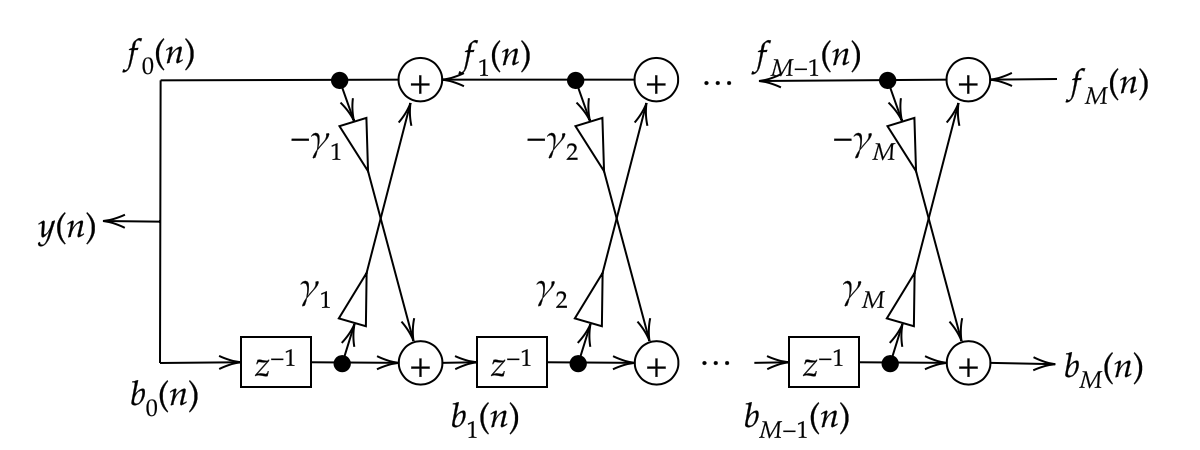
\includegraphics[width=120mm]{./figs/cascaded_lattice_filter_synthesis.png}
    \caption{格子型フィルターの連結(図\ref{cascaded_lattice_filter_synthesis}を再掲)}
  \end{center}
\end{figure}

合成処理部分の実装をリスト\ref{parcor_synthesis}に示す。
\lstinputlisting[linerange={362-379,99999-999999}, firstnumber=362, caption=PARCOR合成フィルター実装(\texttt{ala\char`_predictor.c}), label=parcor_synthesis]{./ALA/ala_predictor.c}

残差計算の時とは異なり、前向き誤差と後ろ向き誤差は両方とも高次から低次の残差に向かって計算するため、前向き誤差と後ろ向き誤差をそれぞれ個別の\texttt{for}文によって更新する必要がない。また、式\ref{parcor_forward_synthesis}に注目すると、前向き誤差は次のサンプルの計算で使われることは無いので配列に記録する必要がなく、単一の変数\texttt{forward\char`_residual}への積和演算を行えば良い。これにより合成処理は予測時よりもわずかに早く計算を行える。

\subsection{MS処理}

CD等に収録されたステレオ音源は、収録環境(マイクの配置、マスタリング等)に依存するがL(左)チャンネルとR(右)チャンネルは互いに\textbf{相関}を持っていることが多い。チャンネル間の相関(他チャンネルの影響)を除去できれば、よりチャンネルの独立性を高めた信号処理を行いやすくなる。チャンネル間の相関を除去する手法の1つに\textbf{MS処理}\index{えむえすしょり@MS処理}がある。MS処理は多数のコーデックで有効性が認められている\cite{wavpacktheory, flac}。本節ではMS処理について概要と実装を説明する。

MS処理は、ある時刻におけるLチャンネル信号$L$とRチャンネル信号$R$を次の式\ref{LRtoM}, \ref{LRtoS}によってM(Mid, ミッド)チャンネル信号$M$とS(Side, サイド)チャンネル信号$S$に変換する。
\begin{eqnarray}
  M &=& L + R \label{LRtoM} \\
  S &=& L - R \label{LRtoS}
\end{eqnarray}

$M,S$はそれぞれ中心、側面成分を示している。一方、相関除去の立場から考えてみると、$M$はLチャンネルとRチャンネルの符号が同一(同相)の成分が強められ、符号が逆(逆相)が弱められた成分、$S$は$M$と逆の性質を持った成分と考えられる。

$M,S$は以下の式\ref{MStoL}, \ref{MStoR}によって$L,R$に戻すことができる。
\begin{eqnarray}
  L &=& (M + S) / 2 \label{MStoL} \\
  R &=& (M - S) / 2 \label{MStoR}
\end{eqnarray}

\subsubsection{MS処理の実装解説}

MS処理の実装をリスト\ref{lr_to_ms}に示す。
\lstinputlisting[linerange={480-504,99999-999999}, firstnumber=480, caption=LR信号をMS信号に変換(\texttt{ala\char`_predictor.c}), label=lr_to_ms]{./ALA/ala_predictor.c}

単純なMS処理の式\ref{LRtoM}, \ref{LRtoS}とは異なり、以下のコードにより変換を行っている。
\lstinputlisting[linerange={496-498,99999-999999}, firstnumber=496, caption=MS変換処理部分(\texttt{ala\char`_predictor.c}), label=lr_to_ms_conversion]{./ALA/ala_predictor.c}

Mチャンネル成分が2で割られている。これで問題なく処理ができる理由は、式\ref{LRtoM}, \ref{LRtoS}による変換の下位1bitは一致しているという整数演算の性質に基づく。整数の下位1bitは奇数か偶数かを示すbitとも捉える事ができる。この整数の奇偶に着目すると、奇数と偶数の加算と減算の結果の奇偶は一致することが分かる。念の為、くどいかもしれないが、奇数と偶数の全ての加減算のパターンを確認してみると、
\begin{eqnarray*}
  奇数 + 奇数 = 偶数 \quad 奇数 - 奇数 = 偶数 \\
  奇数 + 偶数 = 奇数 \quad 奇数 - 偶数 = 奇数 \\
  偶数 + 奇数 = 奇数 \quad 偶数 - 奇数 = 奇数 \\
  偶数 + 偶数 = 偶数 \quad 偶数 - 偶数 = 偶数
\end{eqnarray*}

よって、$M$か$S$の片方の奇偶が分かればもう片方の奇偶を判別できる。この事実を用いれば、$M$か$S$片方の奇偶、つまり下位1bitは冗長な情報となるので削除できる。本実装では$M$チャンネルの下位1bitを右シフトによって削除している\footnote{コメントに記したが、右シフトでないと成立しないことに要注意。例えば、\texttt{L=-741, R=322, M=L+R=-419, S=L-R=-1063}のとき、\texttt{(L+R)>>1}は\texttt{-210}と評価される。\texttt{-210}を1bit左シフトすると\texttt{-420}と評価されるが、下位1bitを\texttt{S}から補えば\texttt{-419}となり、元に戻る。\texttt{(L+R)/2}は\texttt{-209}と評価され、\texttt{M}は元に戻らない。筆者は単純な除算を行って検証してしまい、休日2日が失われた。}。

次に、MS信号をLR信号に戻す処理の実装をリスト\ref{ms_to_lr}に示す。
\lstinputlisting[linerange={506-529,99999-999999}, firstnumber=506, caption=MS信号をLR信号に変換(\texttt{ala\char`_predictor.c}), label=ms_to_lr]{./ALA/ala_predictor.c}

変換処理部分の実装をリスト\ref{ms_to_lr_conversion}に示す。
\lstinputlisting[linerange={522-525,99999-999999}, firstnumber=522, caption=LR復元処理部分(\texttt{ala\char`_predictor.c}), label=ms_to_lr_conversion]{./ALA/ala_predictor.c}

まずSチャンネル成分の下位1bitの情報を使ってMS成分を復元してから、後は式\ref{MStoL}, \ref{MStoR}によってLRチャンネル成分を復元している。

\subsection{プリエンファシス/デエンファシス}

線形予測の前処理として、\textbf{プリエンファシス}\index{ぷりえんふぁしす@プリエンファシス}という処理が行われる事が多い\cite{digitalsoundprocess, linearpredict}。プリエンファシスは、音声の高周波数成分を強調する処理であり、しばしばタップ数1のFIRフィルターで実現される。具体的に処理を式に起こしてみると、時刻$n$における出力$y(n)$は、現在の入力$x(n)$と直前時刻の入力$x(n-1)$を用いて式\ref{pre_emphasis}で定義される。
\begin{eqnarray}
  y(n) = x(n) - \mu x(n-1) \label{pre_emphasis}
\end{eqnarray}

ここで$\mu$はFIRフィルターの係数であり、プリエンファシス処理においては$0.9 \leq \mu \leq 1$の範囲に設定される。もし$\mu=1$ならば式\ref{pre_emphasis}は入力データの差分計算に該当するため、直流成分を完全に打ち消す効果を持つ。

プリエンファシス処理を施したデータを元に戻す処理に\textbf{デエンファシス}がある。これはプリエンファシスとは逆に低周波数成分を強調する処理であり、次の式\ref{de_emphasis_filter}で定義される。
\begin{eqnarray}
  y(n) = x(n) + \mu x(n-1) \label{de_emphasis}
\end{eqnarray}

何故プリエンファシス処理が上手くいくのか、筆者が調べた限り、その定性的な説明はなされていない。一般に、プリエンファシス処理によって、収録時に失われがちな高周波数成分が相対的に持ち上がり、スペクトラムが平坦になるのが良い分析結果をもたらすという説明が多くなされる。\cite{linearpredict}では実験的に、プリエンファシスを使用した場合は、線形予測で得られる係数が安定(発散しにくい状態)になりやすいとの結果を示している。

\subsubsection{プリエンファシスフィルター処理}

プリエンファシスフィルター処理の実装をリスト\ref{pre_emphasis_filter}に示す。
\lstinputlisting[linerange={384-406,99999-999999}, firstnumber=384, caption=プリエンファシスフィルター処理(\texttt{ala\char`_predictor.c}), label=pre_emphasis_filter]{./ALA/ala_predictor.c}

入力データ\texttt{data}をその場で(in-placeで)書き換える関数である。フィルター計算は固定小数乗算を使用しており、式\ref{pre_emphasis}の$\mu$に該当する係数との乗算を、\texttt{(1 << coef\char`_shift) - 1}との乗算処理と、\texttt{coef\char`_shift}の右シフト処理に分けて実現している。\texttt{ALA}バージョン1.0.0では、\texttt{coef\char`_shift}は\texttt{5}に設定されているため、フィルター係数$\mu$の値は$\mu = (2^{5} - 1) / 2^{5} = 31 / 32 = 0.96875$に相当する。

\subsubsection{デエンファシスフィルター処理}

デエンファシスフィルター処理の実装をリスト\ref{de_emphasis_filter}に示す。
\lstinputlisting[linerange={408-426,99999-999999}, firstnumber=408, caption=デエンファシスフィルター処理(\texttt{ala\char`_predictor.c}), label=de_emphasis_filter]{./ALA/ala_predictor.c}

デエンファシスフィルター処理は簡単である。式\ref{de_emphasis}で示したように、前のサンプル値にフィルター係数を乗じ、現在のサンプル値に加算するだけで良い。

\subsection{残差のエントロピー観察}

本節ではMS処理、プリエンファシス、PARCOR予測の3つの予測手法によって、どれほど音声データのエントロピーが変化するかを観察する。

\subsubsection{元の信号と残差の分布}

信号の分布は、入力\texttt{wav}の元の信号(残差計算前)とその残差の計算結果に対してPCM値の出現頻度を計測することで観察した。頻度の絶対値は音源により異なるため、出現頻度の総和を取って出現頻度を割ることで経験確率を算出した。

表\ref{wavs_8bitentropy}で挙げた8個の\texttt{wav}ファイルに対して信号の分布を計測した結果を図\ref{idonochawan_dist}-\ref{calendergirl_dist}に示す。グラフにおいて、横軸(PCMの値)の範囲は-2048から2048に制限し、縦軸(経験確率)は差を見やすくするために対数軸を用いている。
\begin{figure}[htbp]
  \begin{center}
    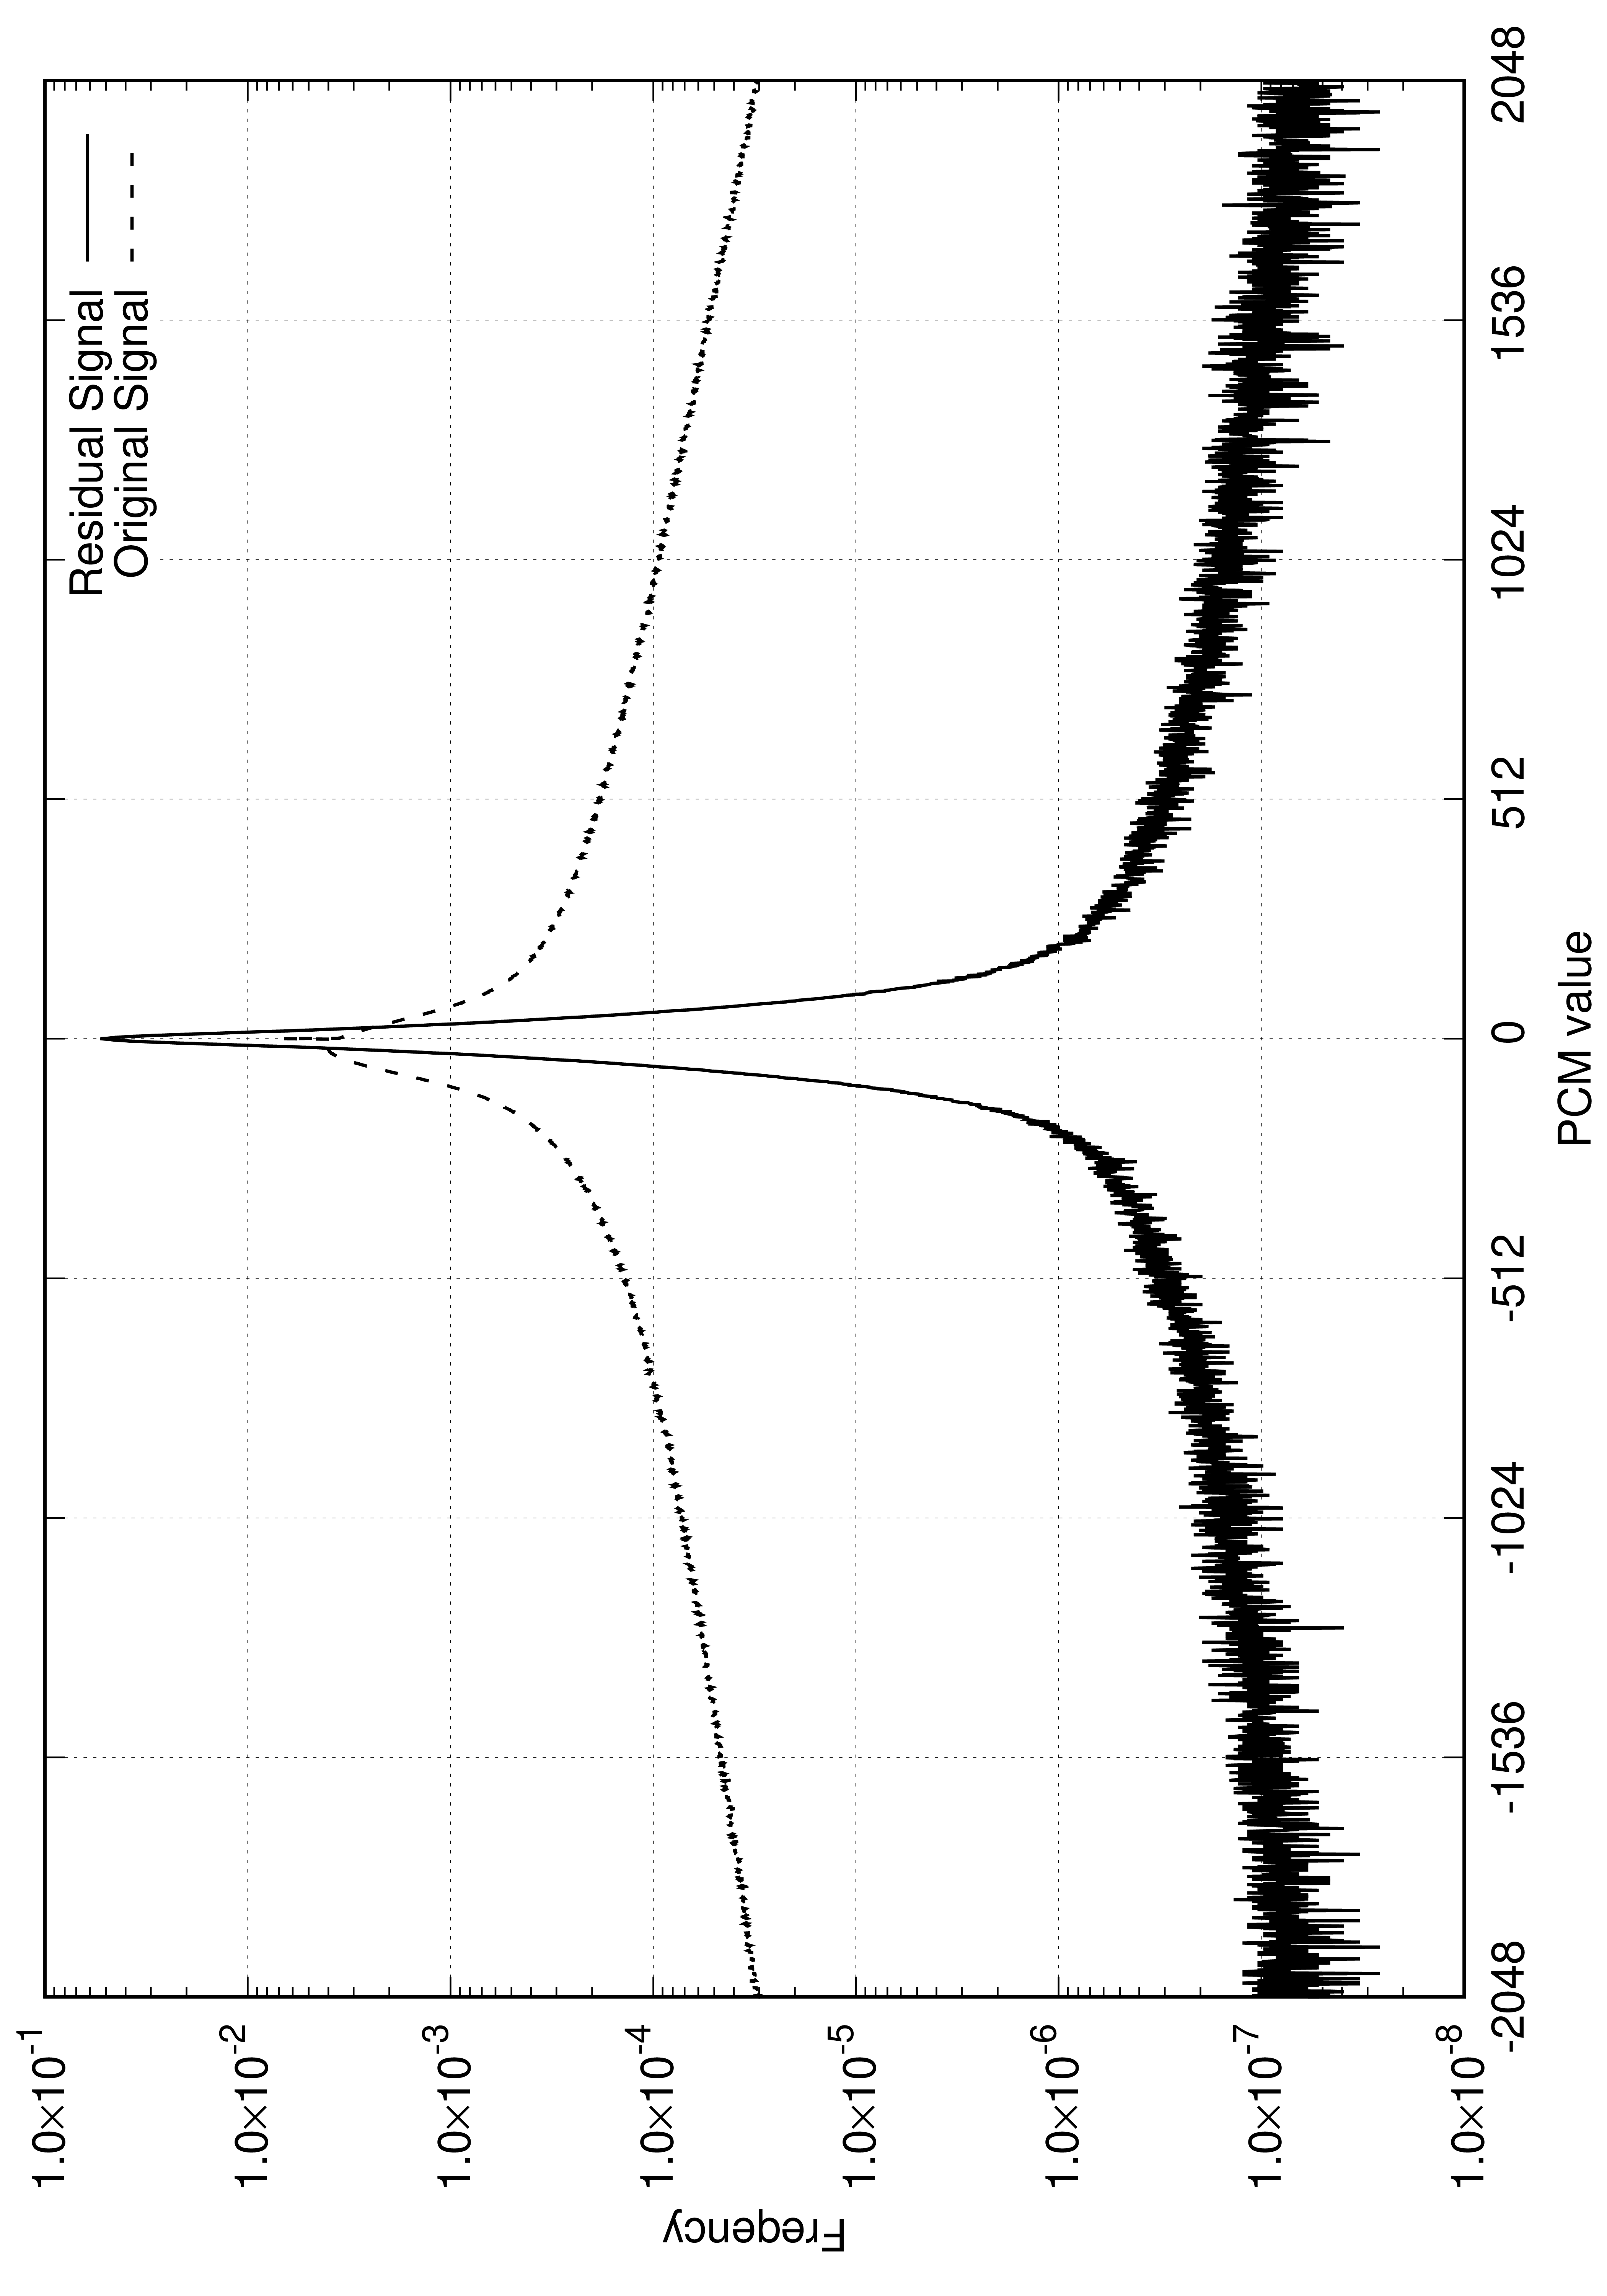
\includegraphics[width=80mm,angle=-90]{./figs/idonochawan_dist.png}
    \caption{\texttt{4-02 井戸の茶椀.wav}に対する信号分布計測結果} \label{idonochawan_dist}
  \end{center}
  \begin{center}
    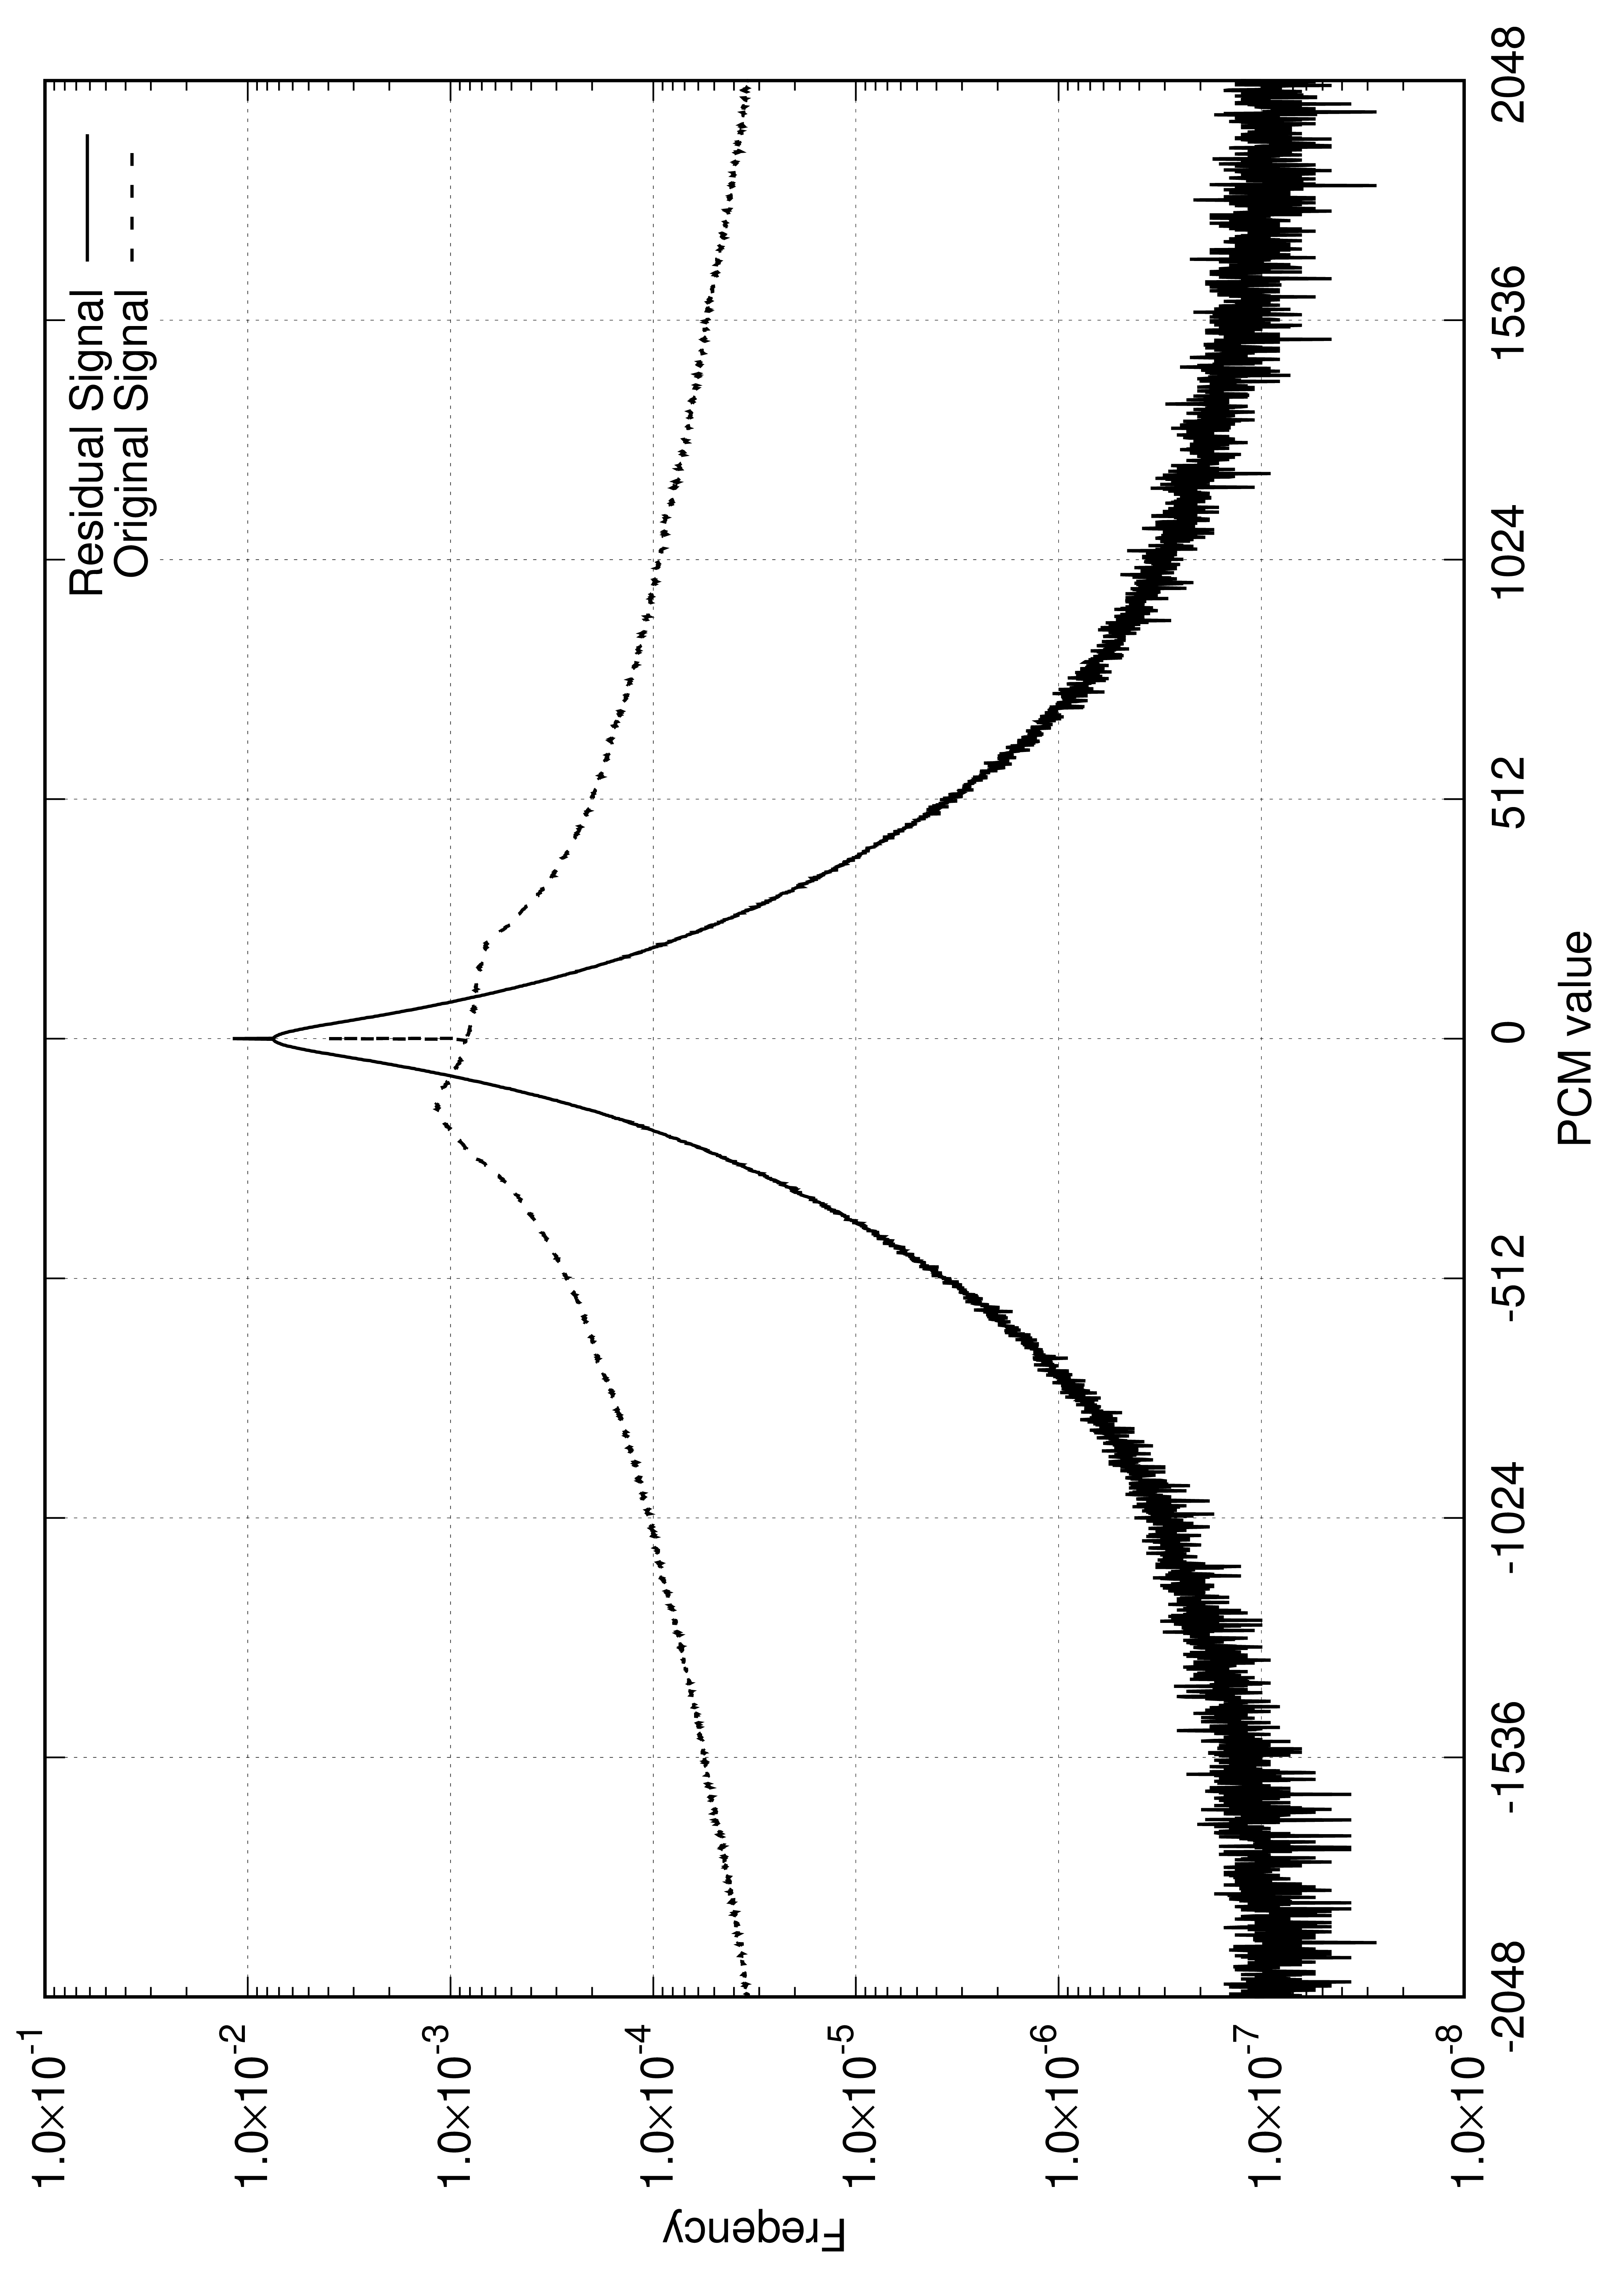
\includegraphics[width=80mm,angle=-90]{./figs/kaendaiko_dist.png}
    \caption{\texttt{1-01 火焔太鼓.wav}に対する信号分布計測結果} \label{kaendaiko_dist}
  \end{center}
\end{figure}
\begin{figure}[htbp]
  \begin{center}
    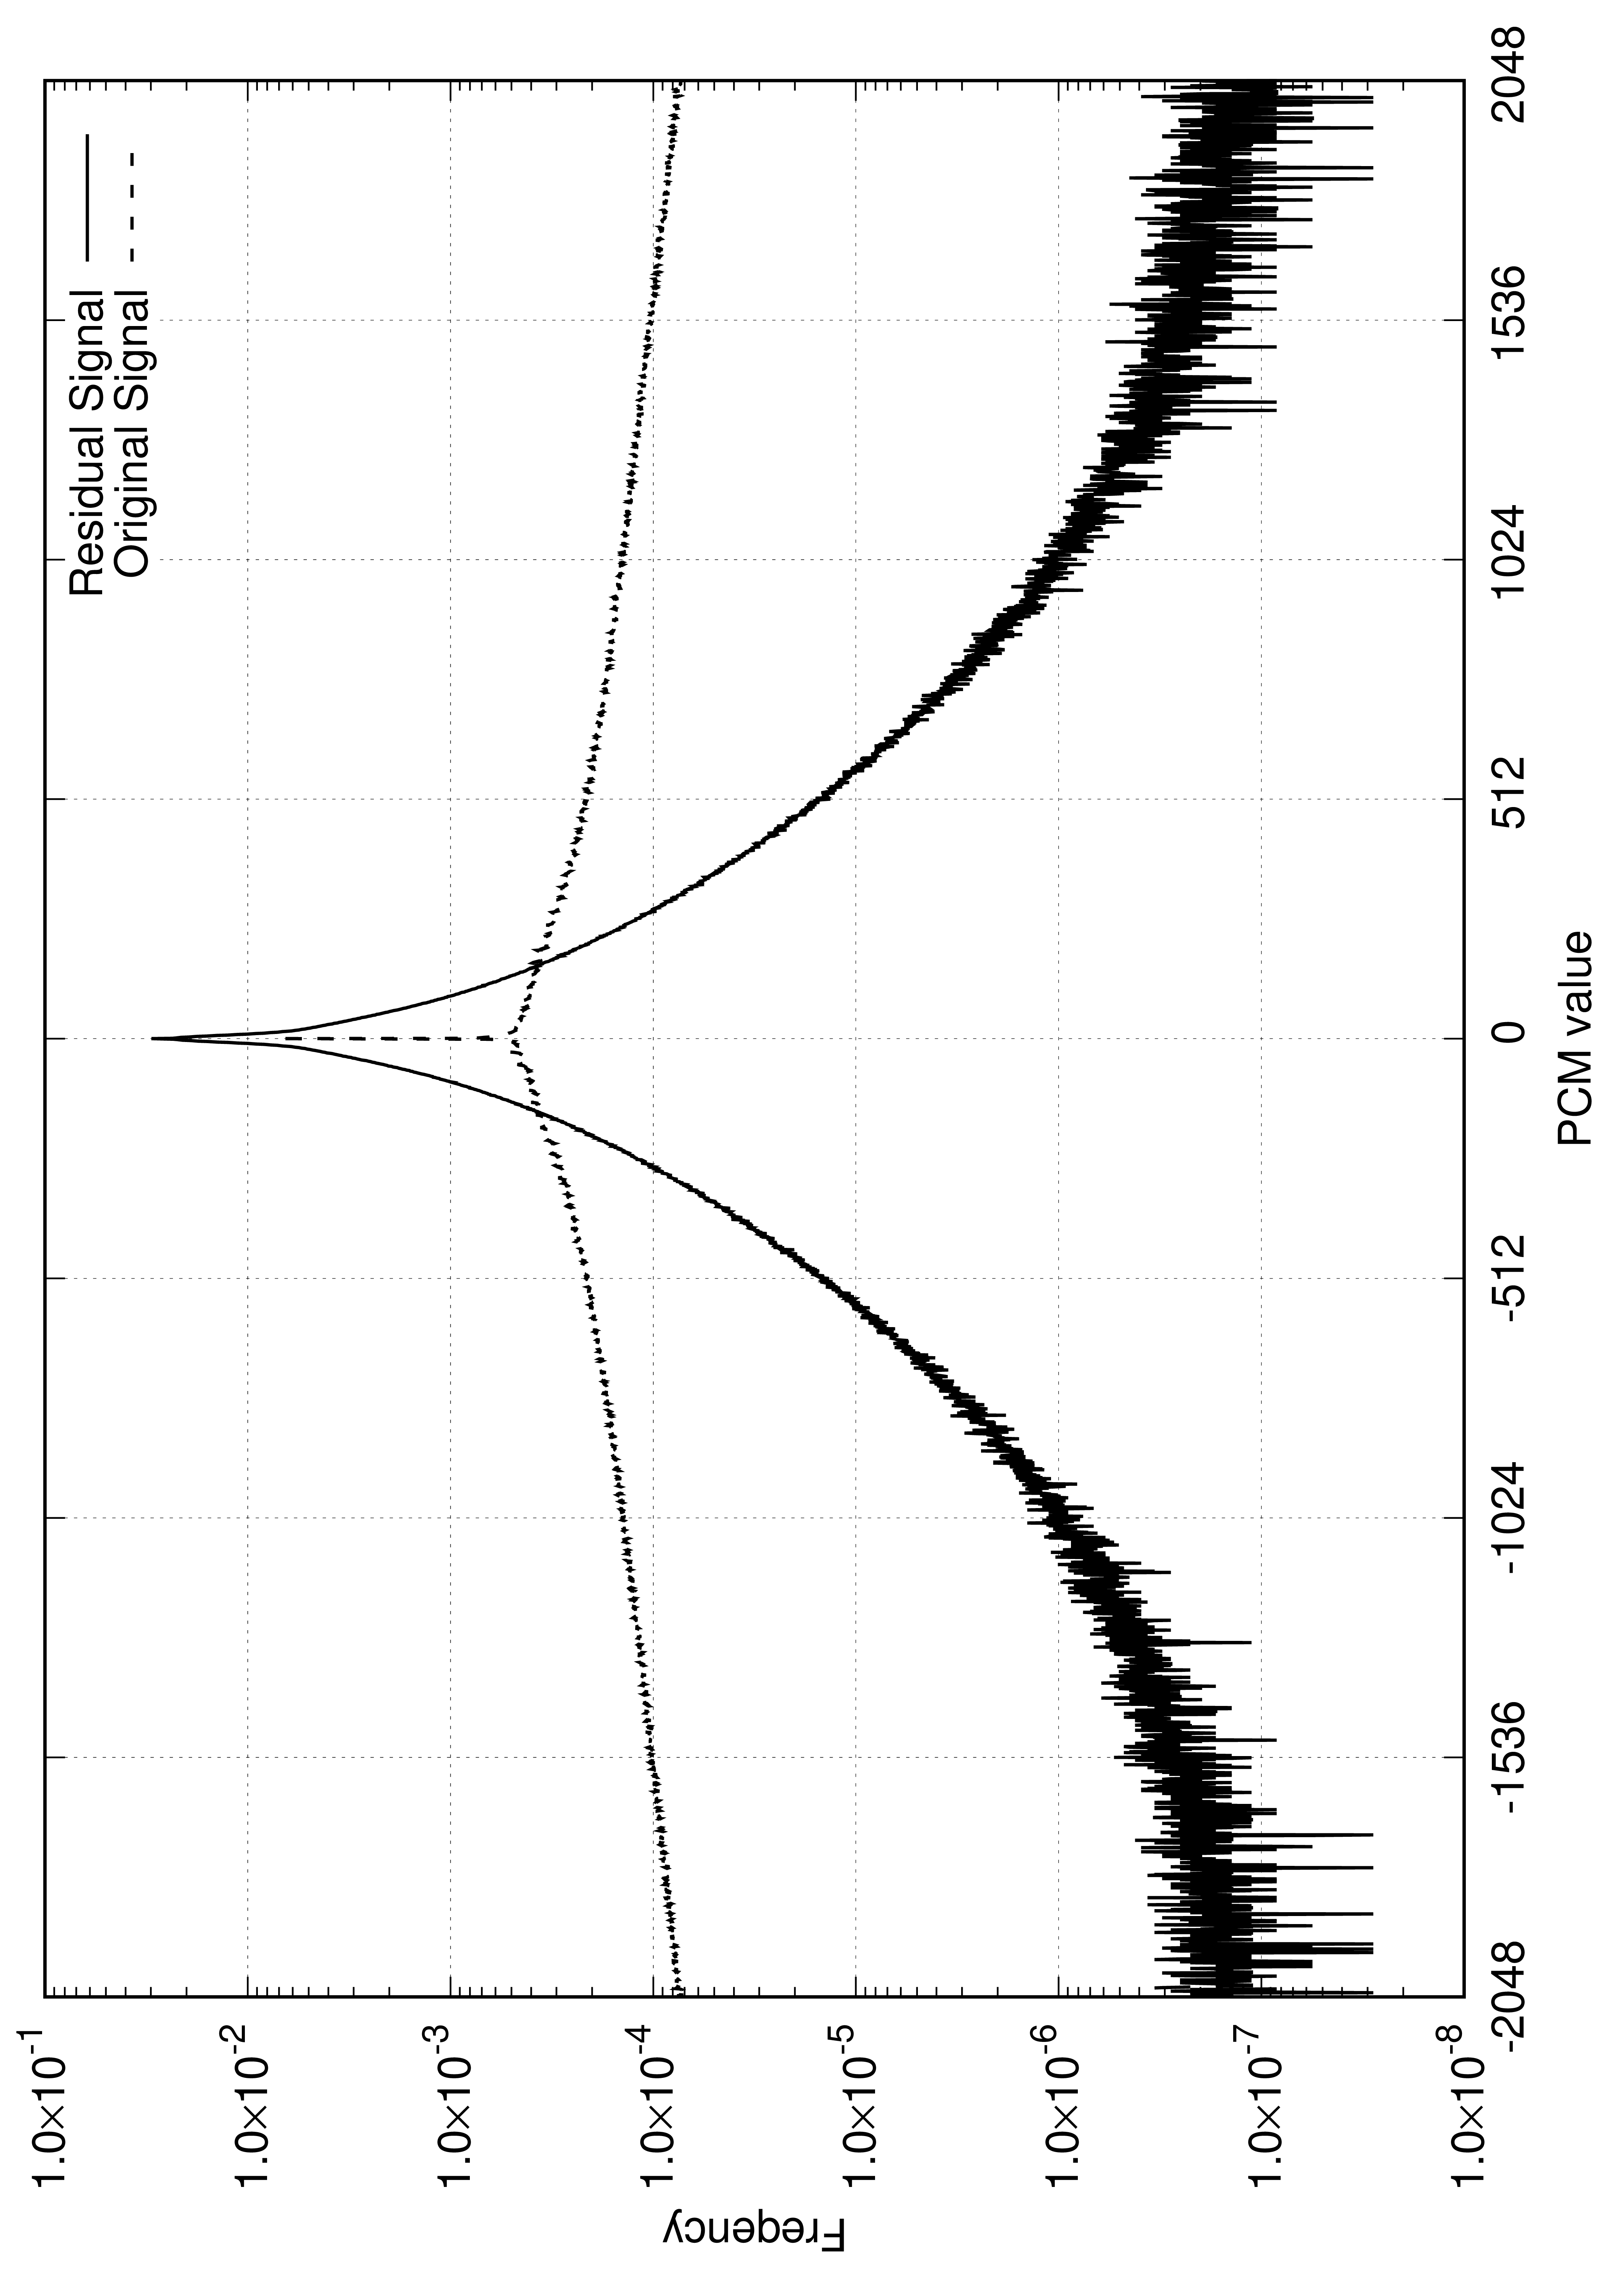
\includegraphics[width=80mm,angle=-90]{./figs/mysong_dist.png}
    \caption{\texttt{02 My Song.wav}に対する信号分布計測結果} \label{mysong_dist}
  \end{center}
  \begin{center}
    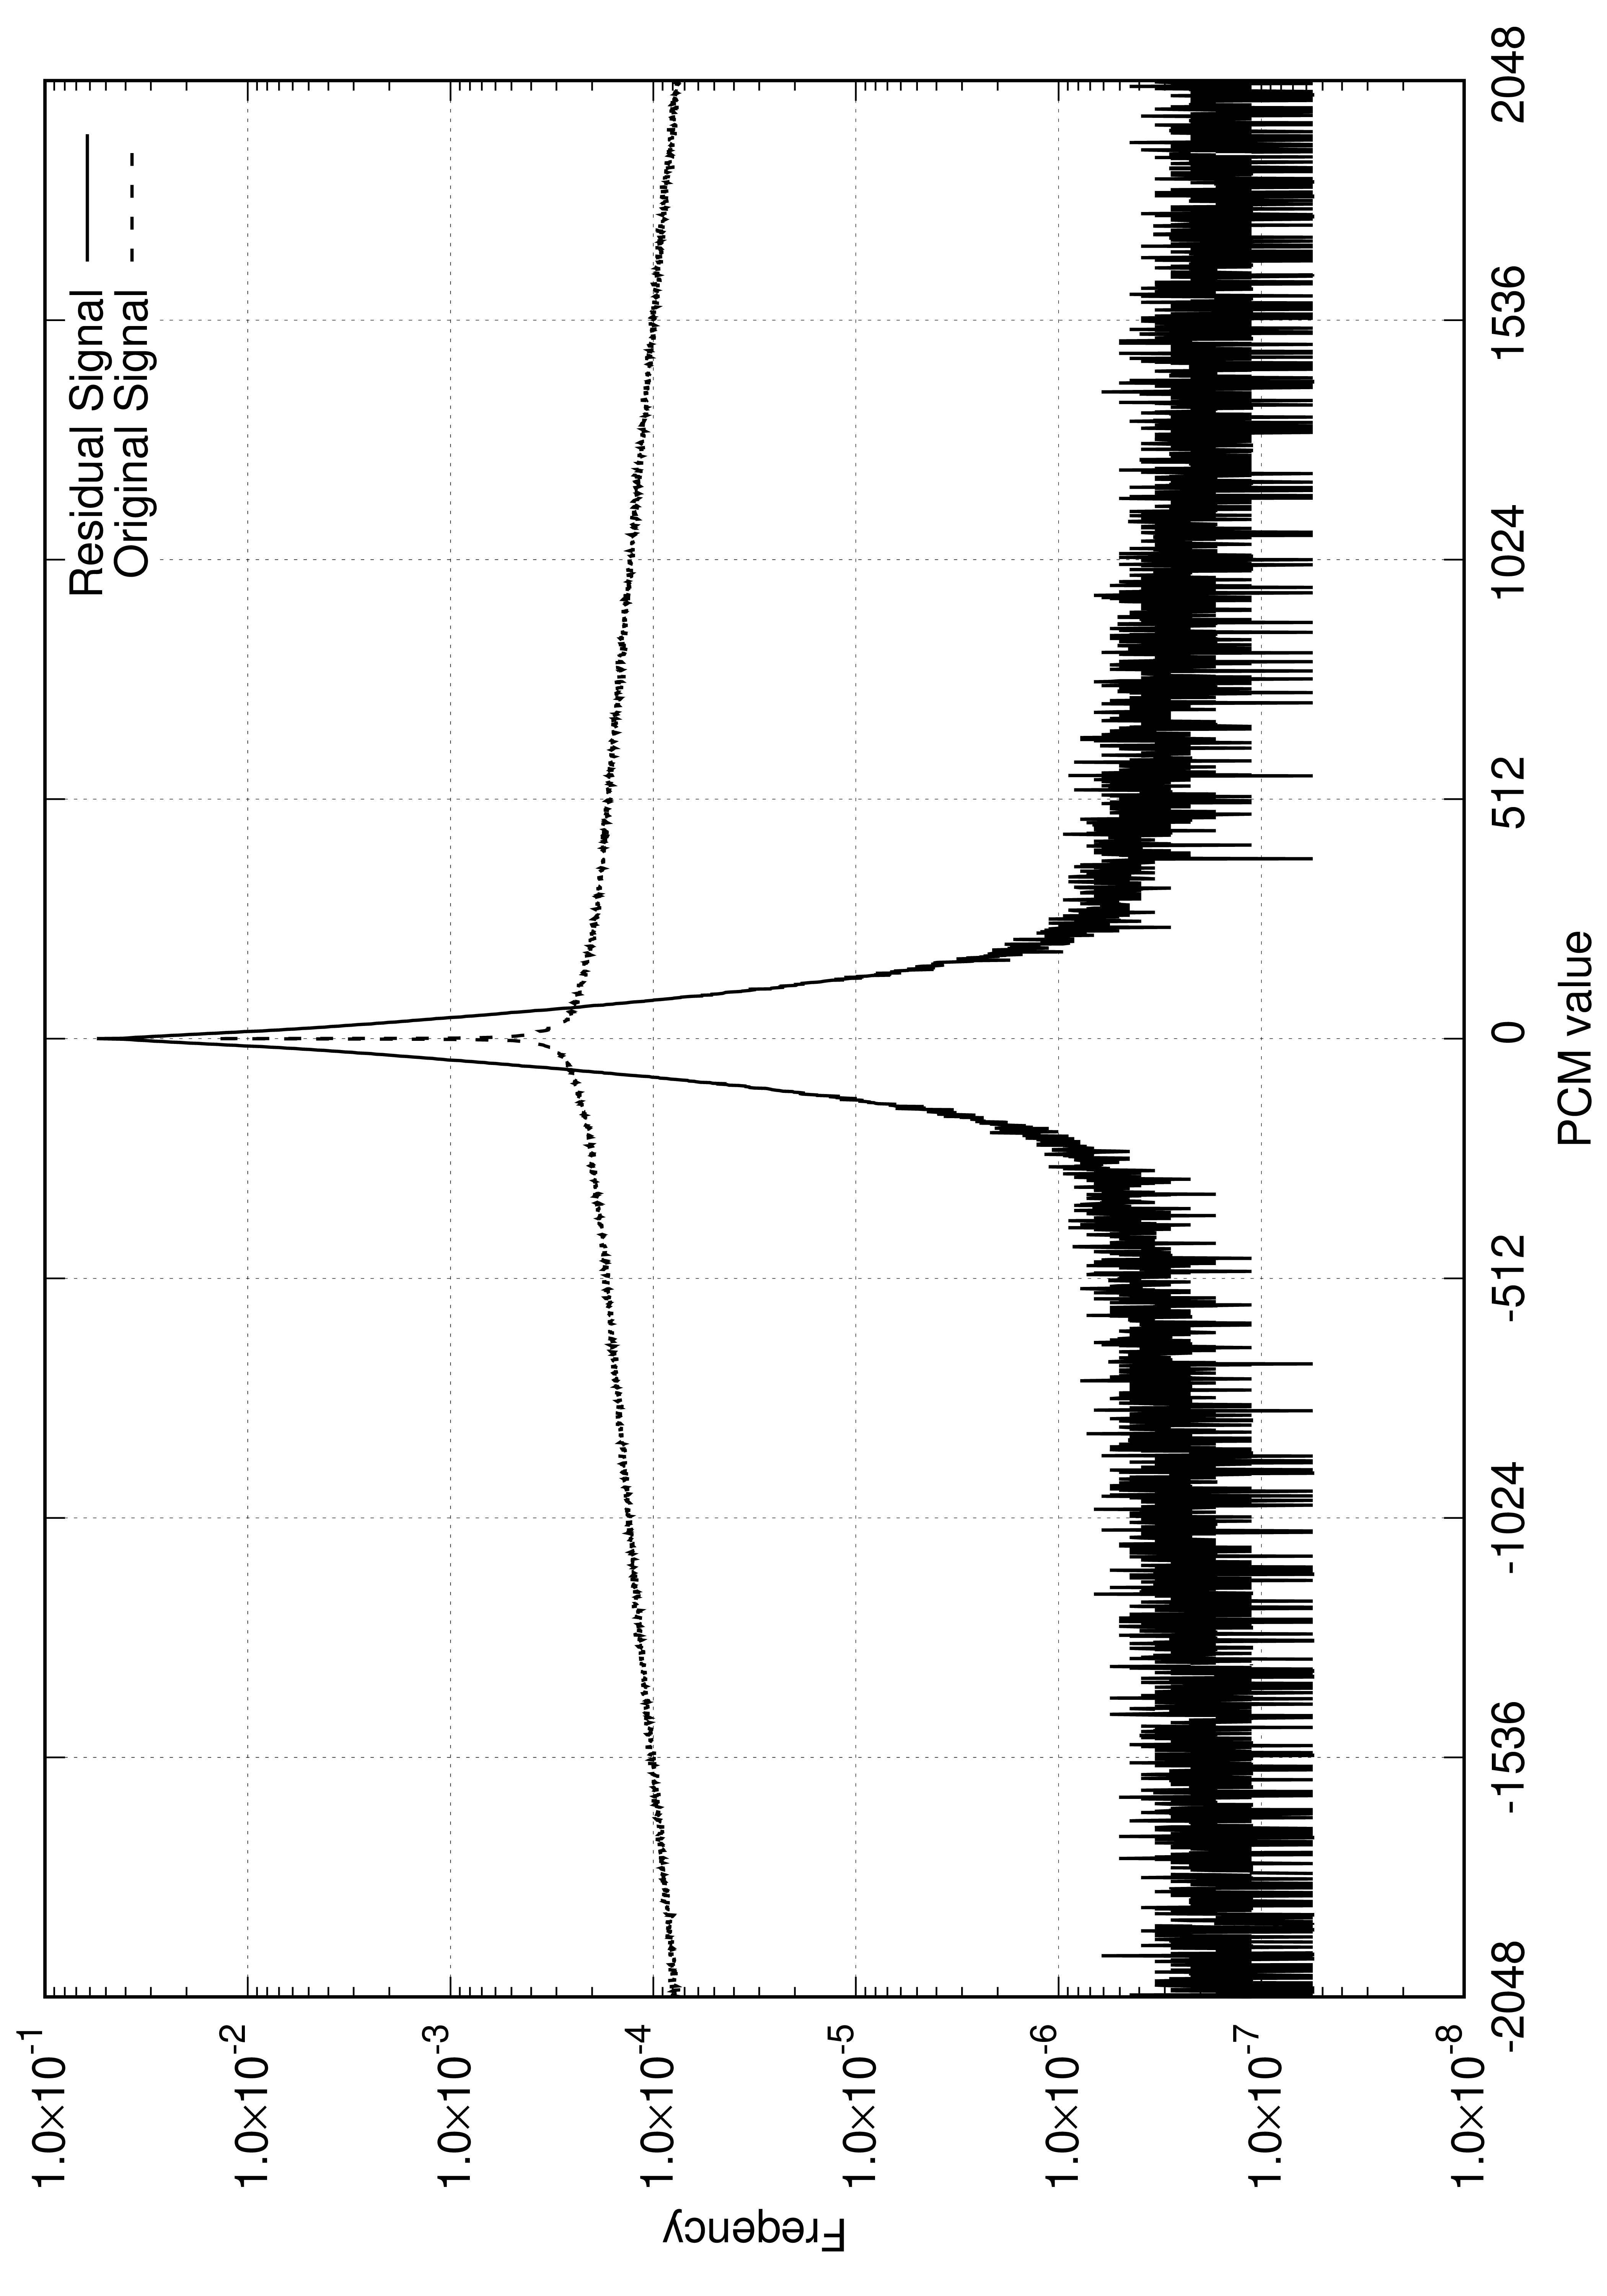
\includegraphics[width=80mm,angle=-90]{./figs/ruriko_dist.png}
    \caption{\texttt{09 瑠璃子.wav}に対する信号分布計測結果} \label{ruriko_dist}
  \end{center}
\end{figure}
\begin{figure}[htbp]
  \begin{center}
    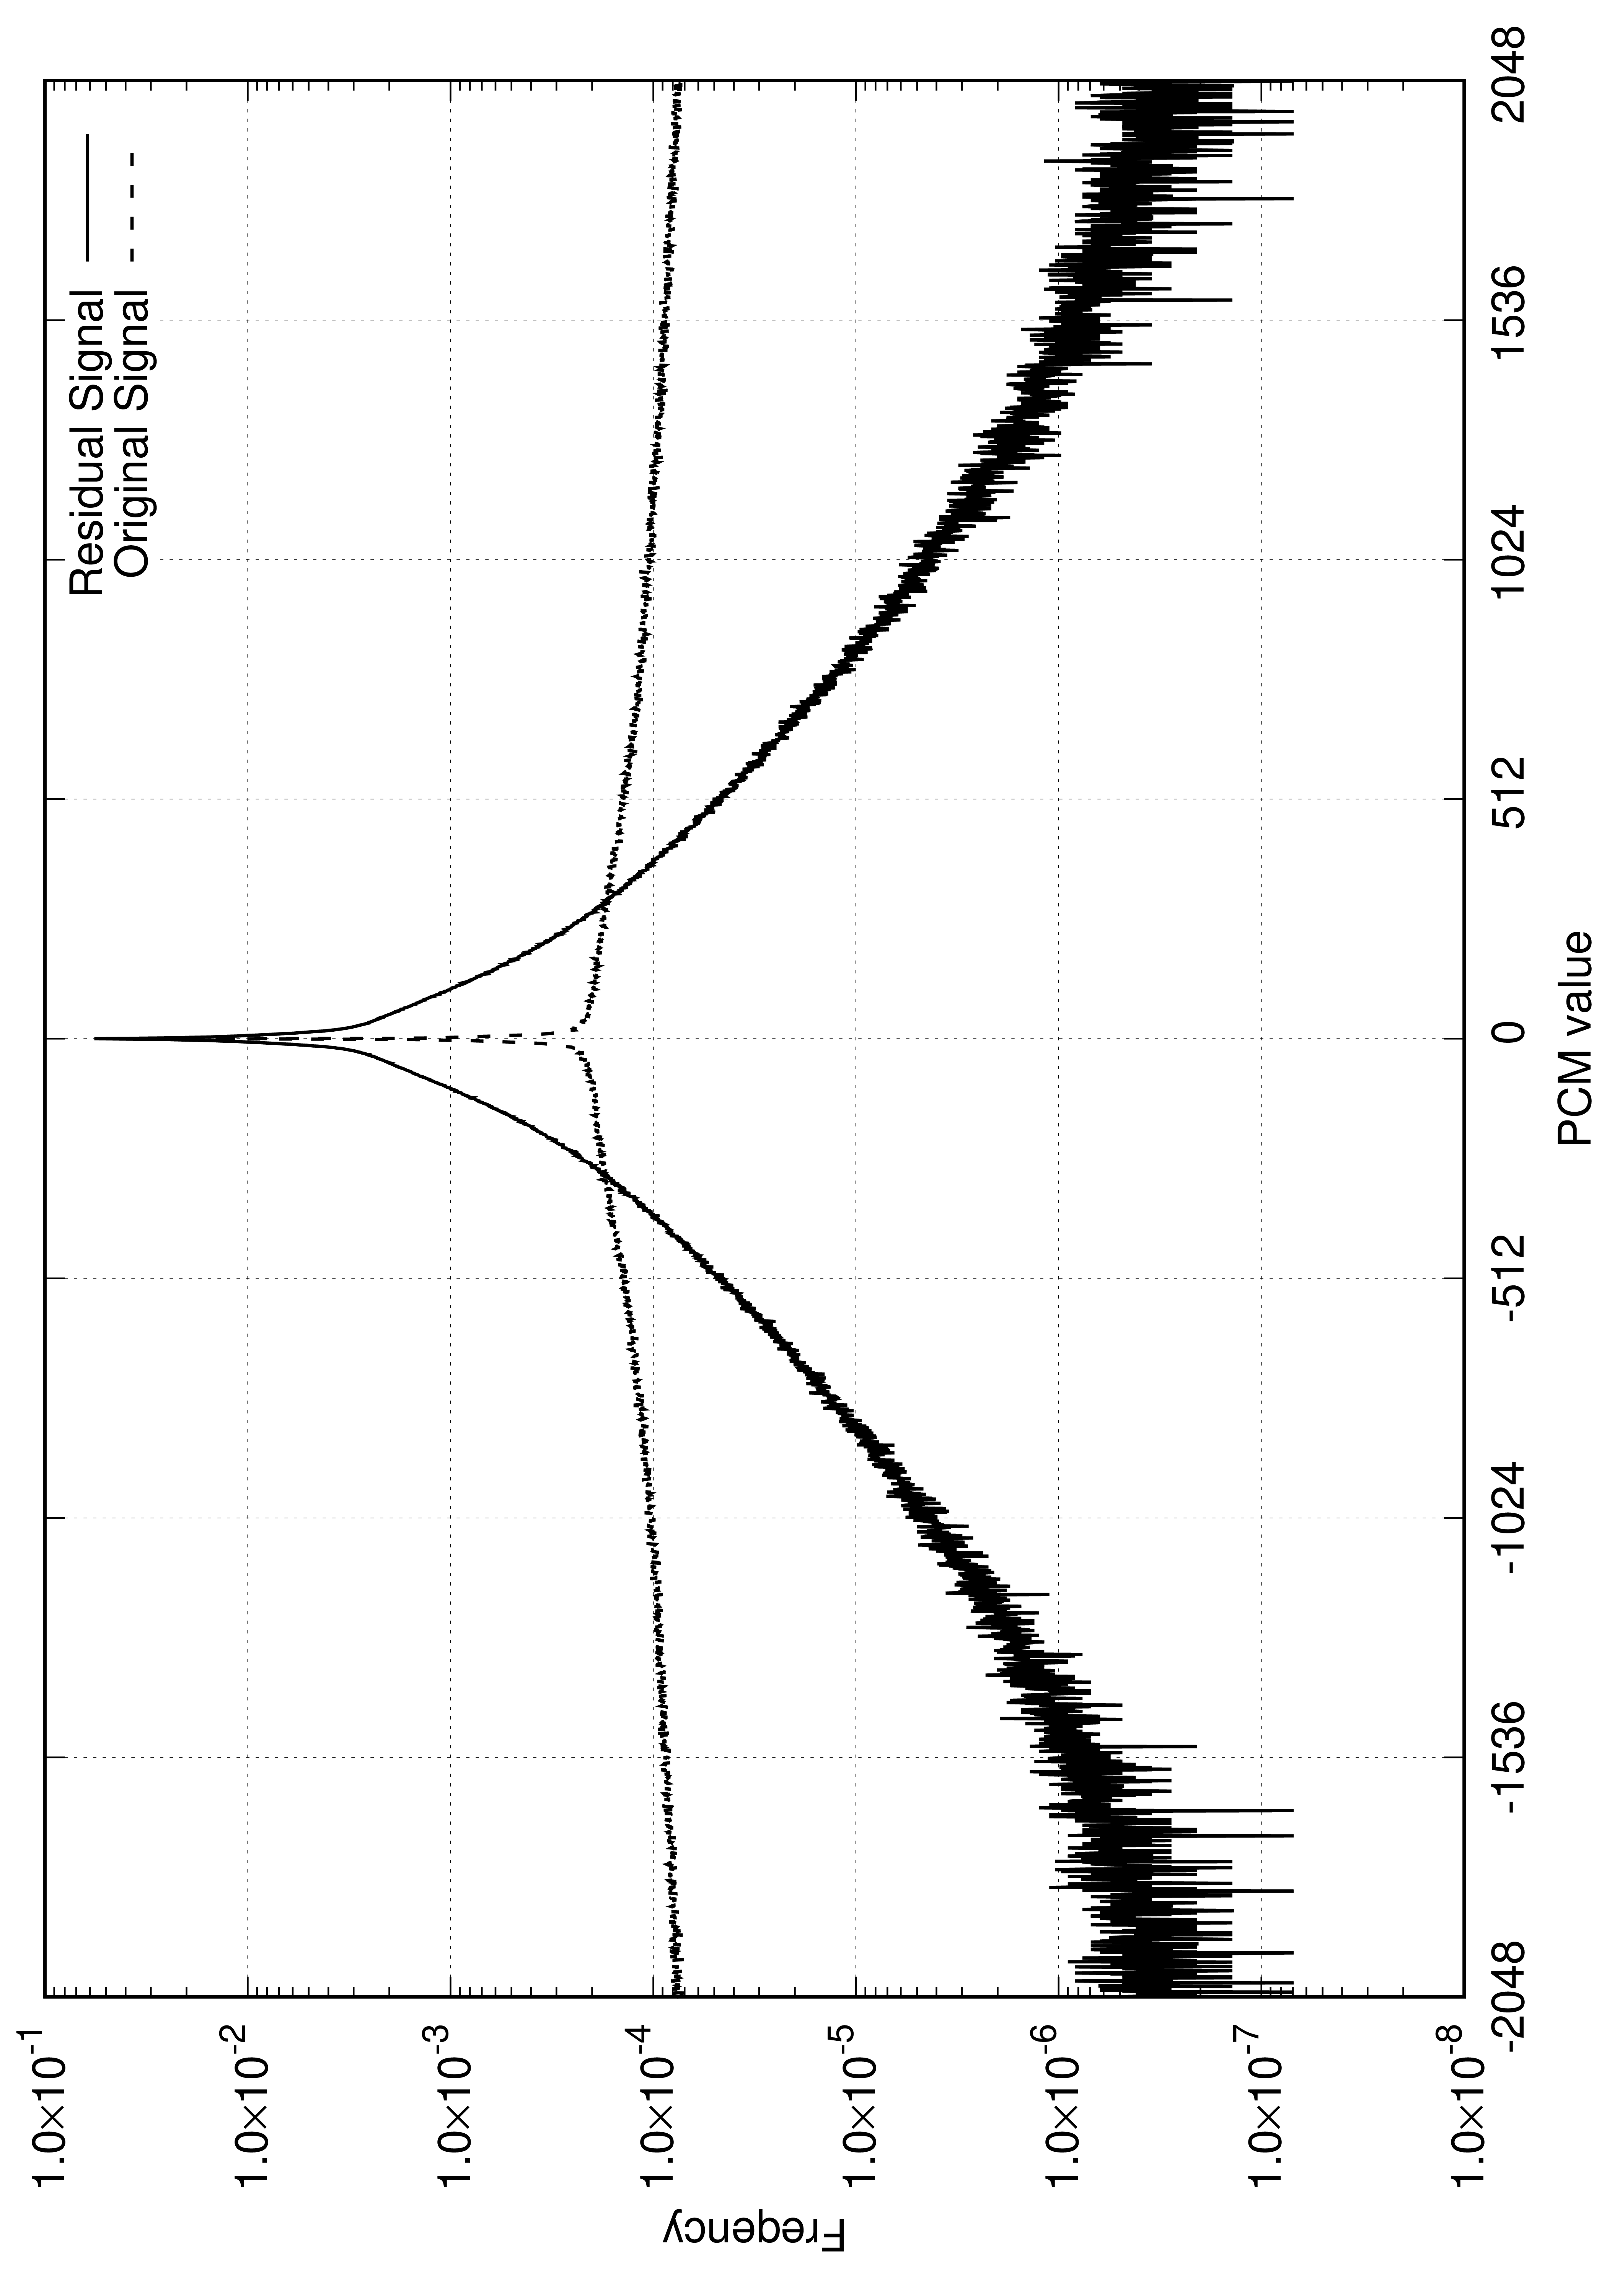
\includegraphics[width=80mm,angle=-90]{./figs/jibundakenokagayaki_dist.png}
    \caption{\texttt{30-自分だけの輝き.wav}に対する信号分布計測結果} \label{jibundakenokagayaki_dist}
  \end{center}
  \begin{center}
    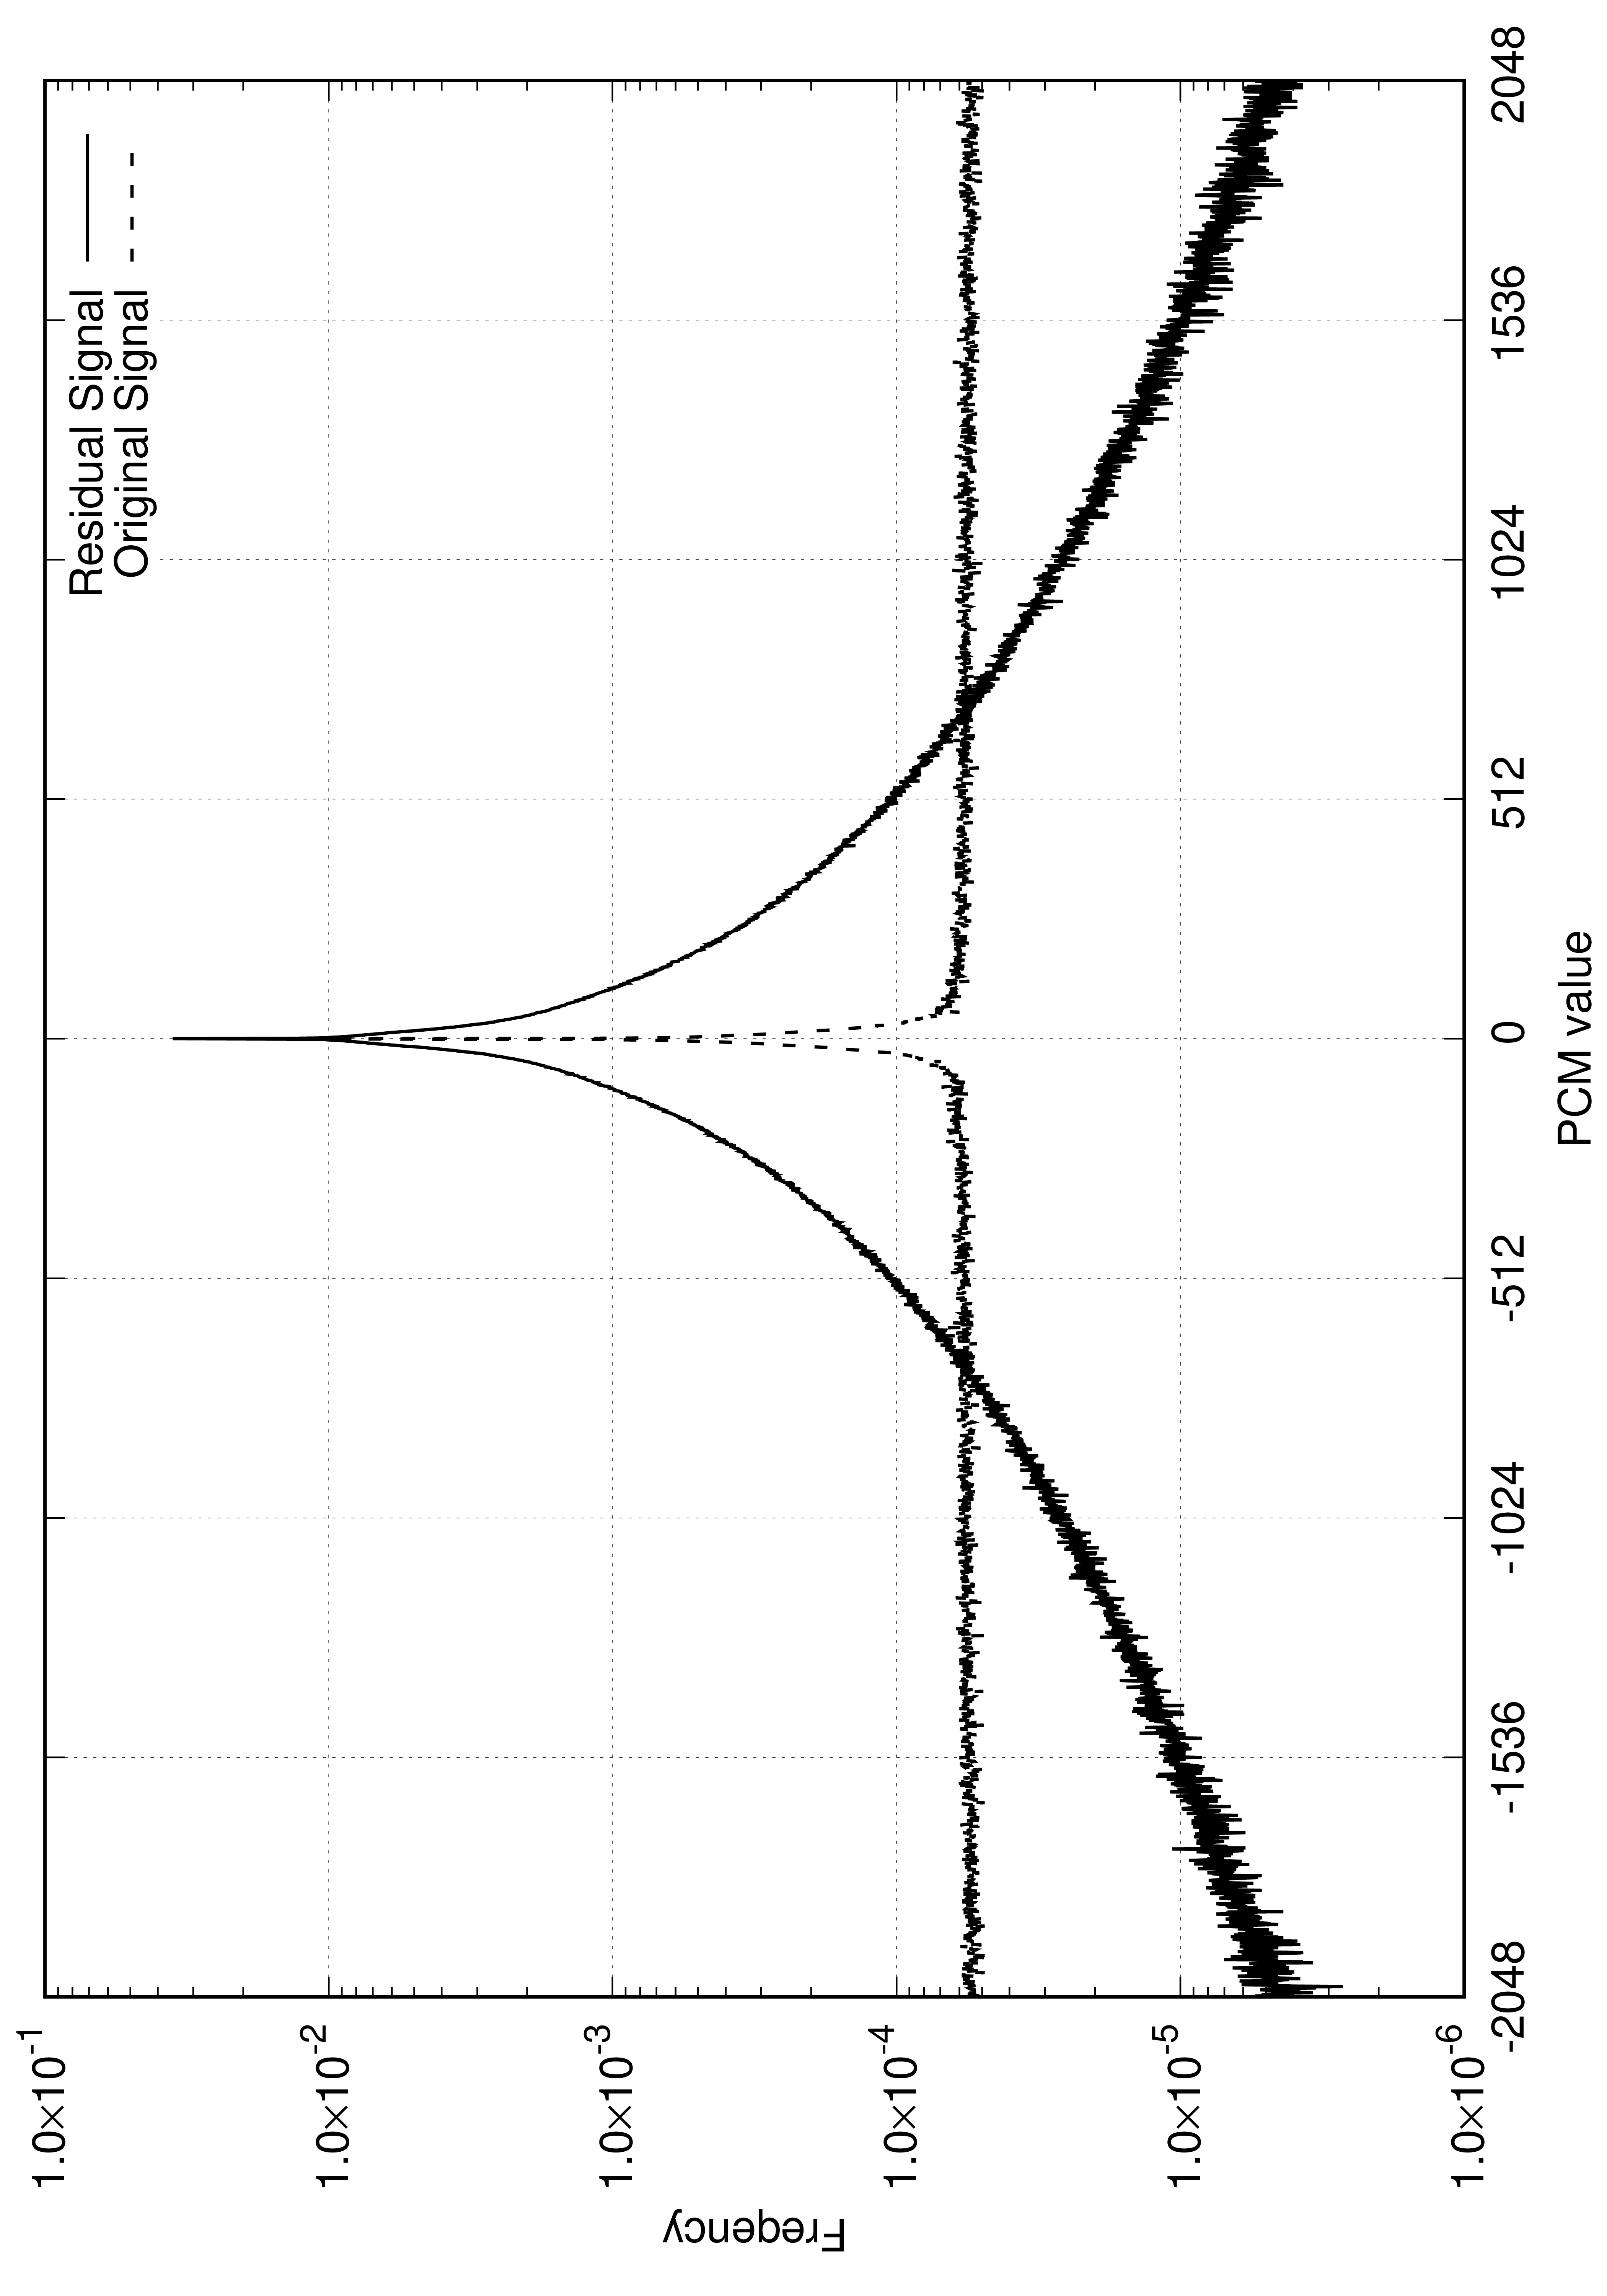
\includegraphics[width=80mm,angle=-90]{./figs/kasanerudoryoku_dist.png}
    \caption{\texttt{29-重ねる努力.wav}に対する信号分布計測結果} \label{kasanerudoryoku_dist}
  \end{center}
\end{figure}
\begin{figure}[htbp]
  \begin{center}
    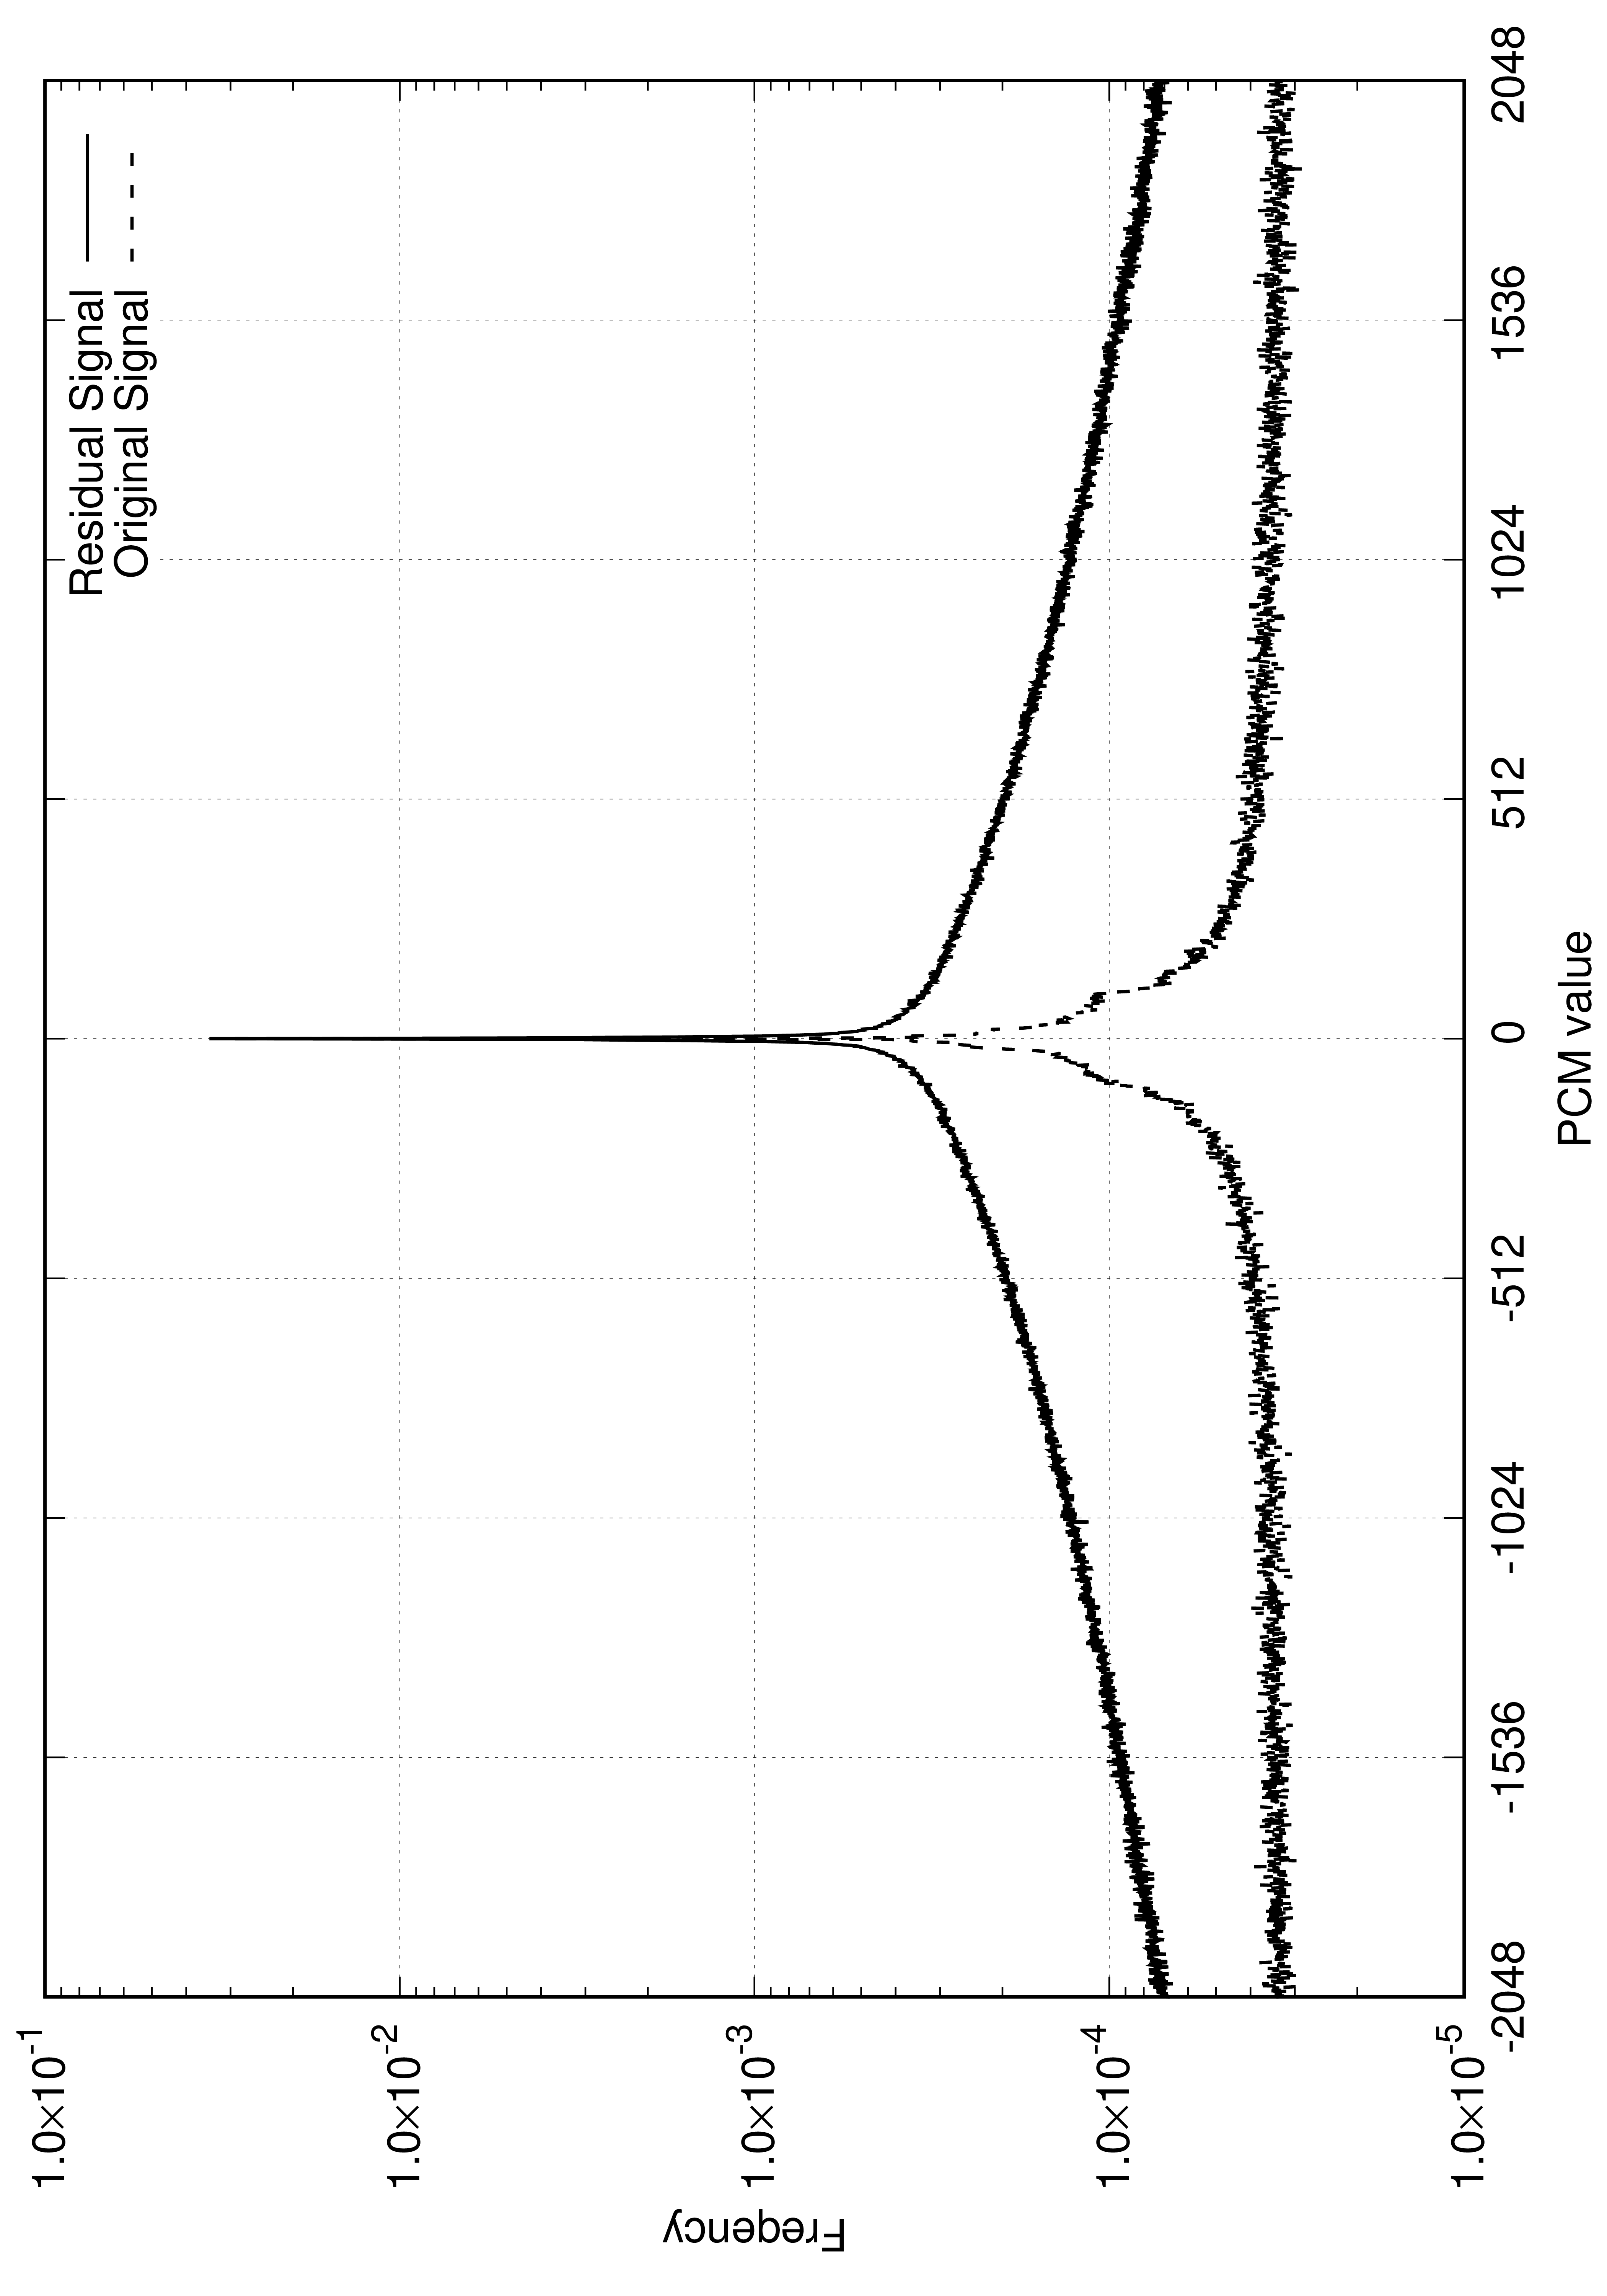
\includegraphics[width=80mm,angle=-90]{./figs/letsaikatsu_dist.png}
    \caption{\texttt{4-02 Let’s アイカツ!(Short サイズ).wav}に対する信号分布計測結果} \label{letsaikatsu_dist}
  \end{center}
  \begin{center}
    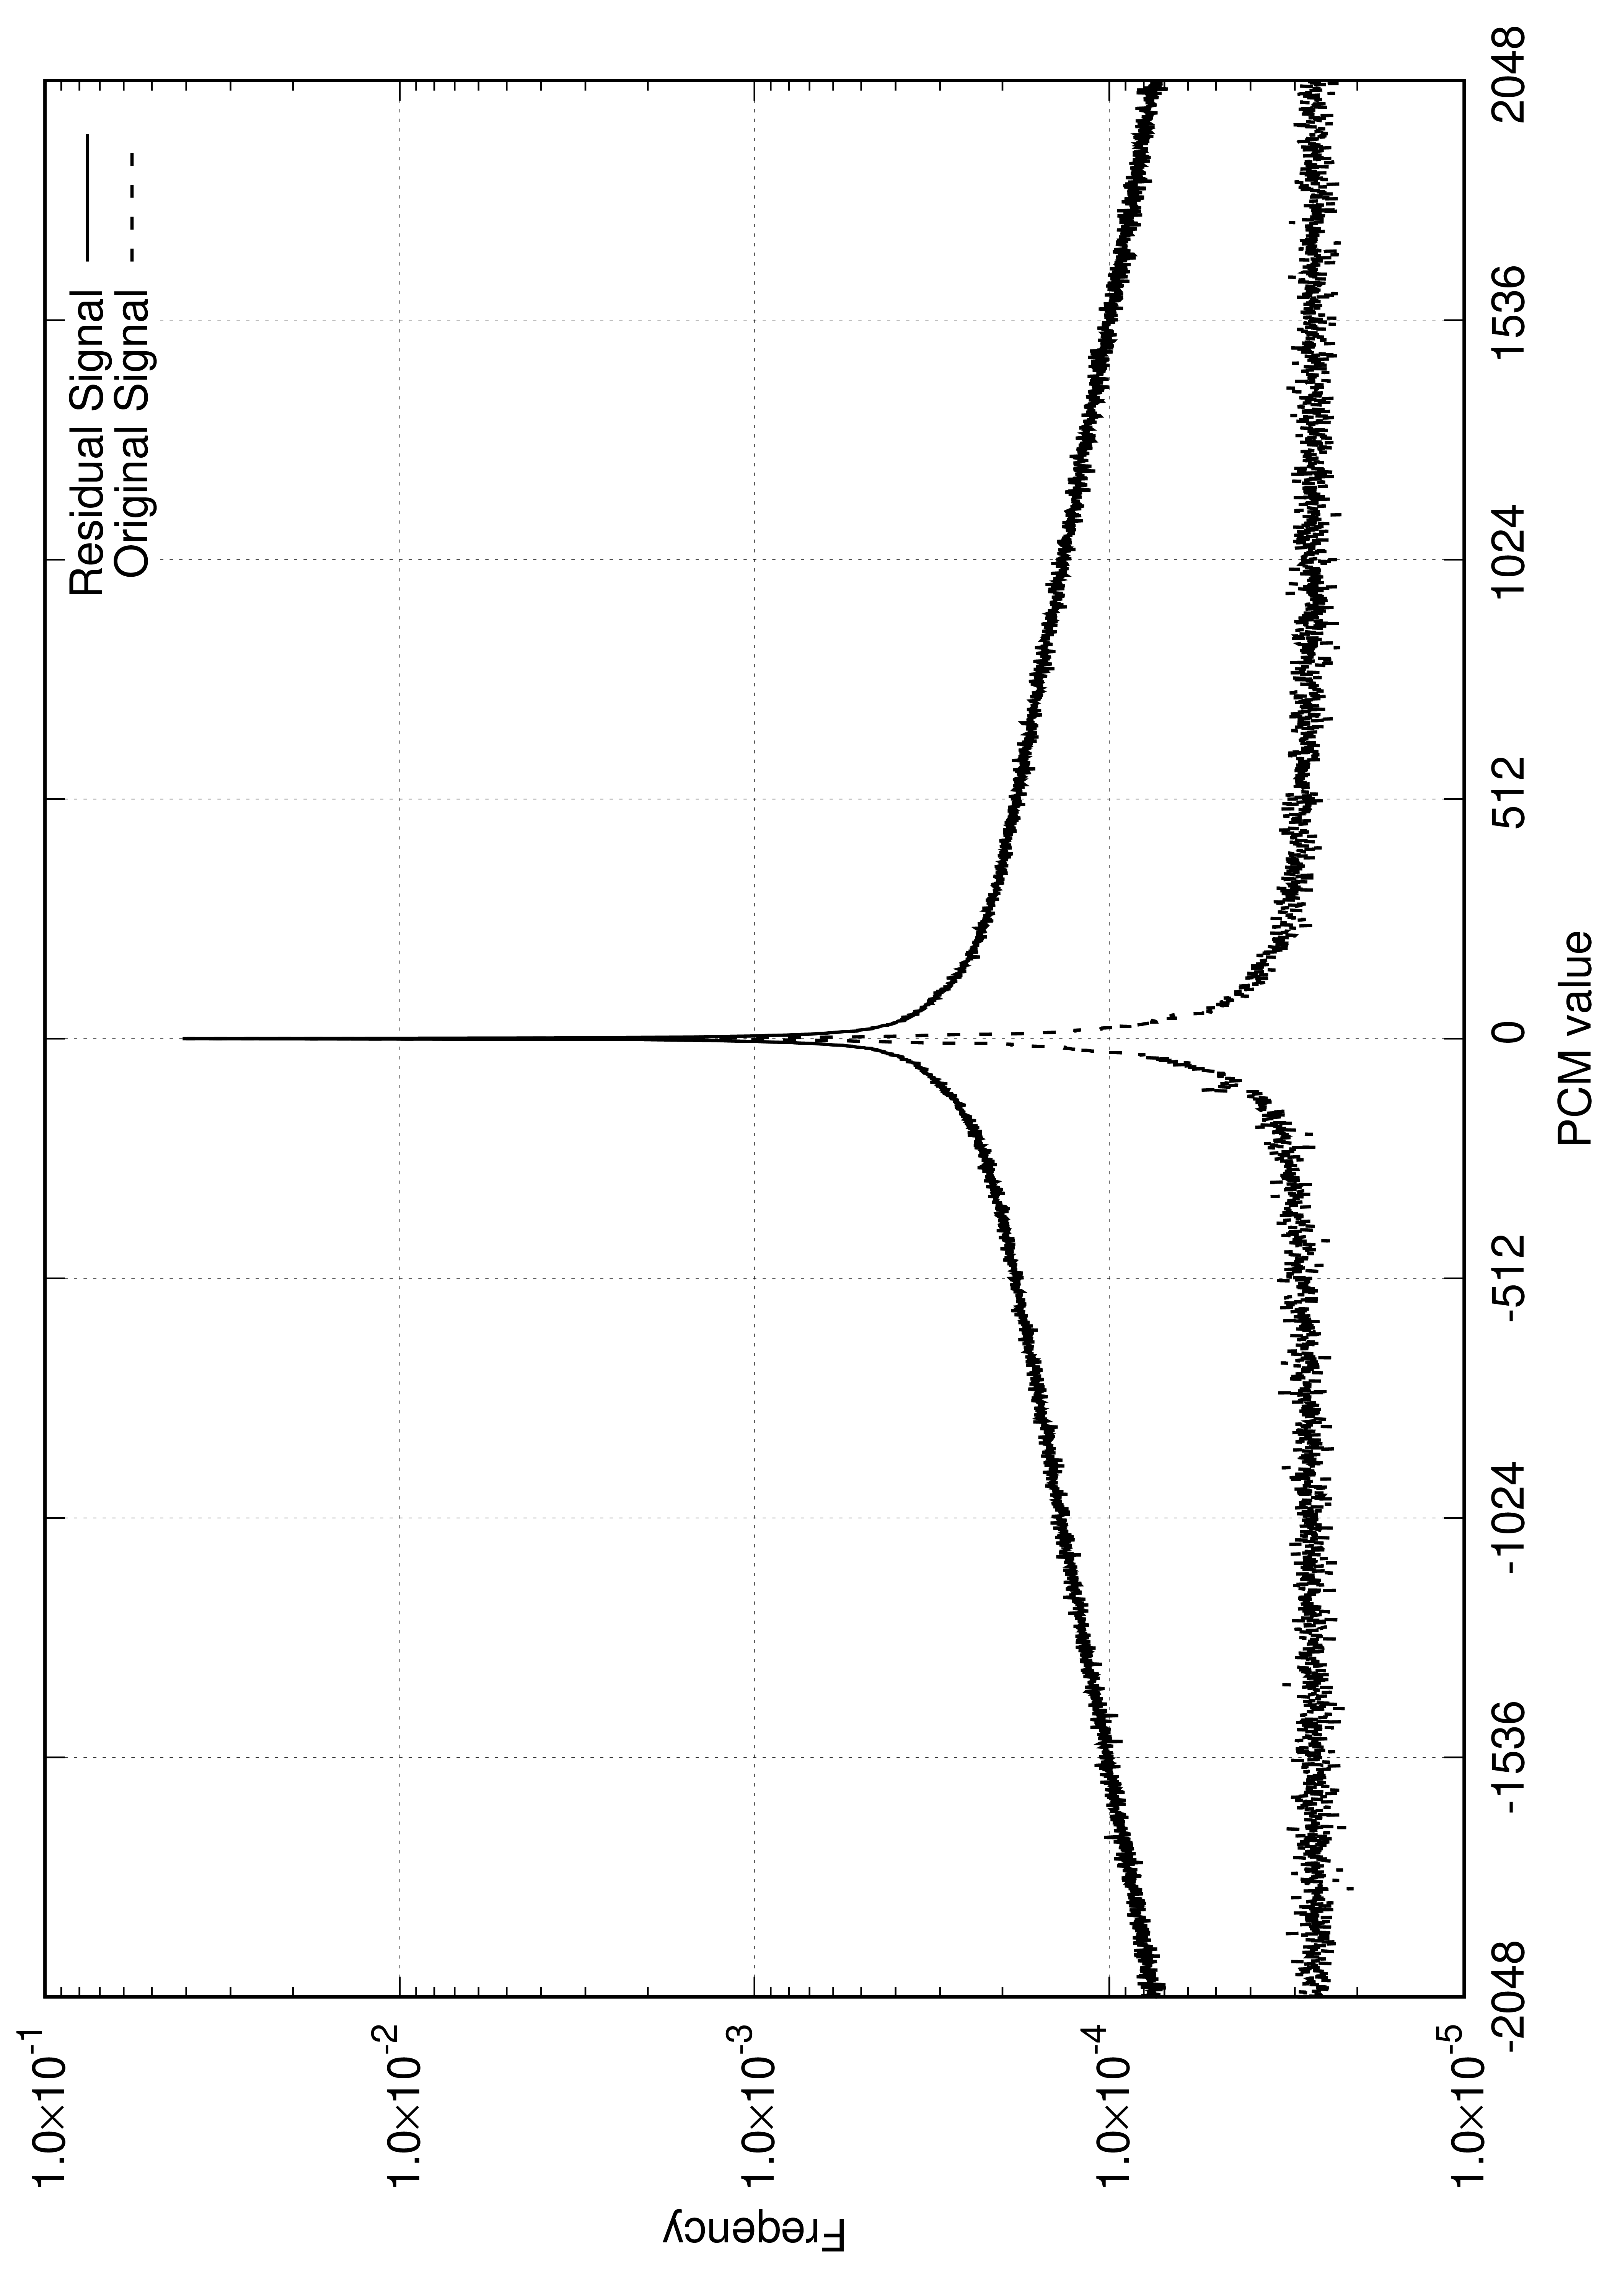
\includegraphics[width=80mm,angle=-90]{./figs/calendergirl_dist.png}
    \caption{\texttt{5-02 カレンダーガール(TV-size).wav}に対する信号分布計測結果} \label{calendergirl_dist}
  \end{center}
\end{figure}

全体的に、残差計算後の分布の方が0における頻度ピーク値が大きく、また、分布の0から離れたところの頻度(裾野)が鋭く減少している事が読み取れる。これは、図\ref{golomb_code_is_geometric_distribution}で見た幾何分布の概形に近く、よりエントロピー符号化に適した分布に変換できていることを意味する。

ファイル個別に気になる点を述べる。\texttt{1-01 火焔太鼓.wav}の元の信号の分布は奇特である。0にピークはあるものの、次の緩やかなピークが$-100$周辺に存在する。これは、収録時に発生している背景ノイズと、直流成分(オフセット)の影響を受けているものと考えられる。
振幅値の振れ幅が大きい\texttt{4-02 Let’s アイカツ!(Short サイズ).wav}と\texttt{5-02 カレンダーガール(TV-size).wav}では、他の分布と異なり残差の減衰が緩やか(裾野が広い)だが、減衰が早いためグラフの横軸を$[-4000, 4000]$まで広げた時に残差の頻度の方が小さくなっていることを確認した。

\subsubsection{残差計算前後でのエントロピーの変化}

残差計算前後でのエントロピーの計算結果を表\ref{wavs_residual_16bitentropy}に示す。表\ref{wavs_8bitentropy}の計測を行った際はデータを1バイト(8bit)に区切って計測していたが、ここではPCMのbit幅(16bit)に区切って計測を行ったため、残差計算前のエントロピー値が表\ref{wavs_8bitentropy}と異なることに注意いただきたい。
\begin{table}[htbp]
  \begin{center}
    \caption{残差計算前後のエントロピー計算結果} \label{wavs_residual_16bitentropy}
    \begin{tabular}{|l|c|c|}
      \hline
      ファイル名 & 元の信号[byte] & 残差[byte] \\ \hline
      \texttt{4-02 井戸の茶椀.wav}                   & 11.04 &  5.44  \\ \hline
      \texttt{1-01 火焔太鼓.wav}                     & 11.91 &  7.88  \\ \hline
      \texttt{02 My Song.wav}                        & 13.04 &  7.86  \\ \hline
      \texttt{09 瑠璃子.wav}                         & 13.66 &  6.01  \\ \hline
      \texttt{30-自分だけの輝き.wav}                 & 13.73 &  8.27  \\ \hline
      \texttt{29-重ねる努力.wav}                     & 14.59 &  9.42  \\ \hline
      \texttt{4-02 Let's アイカツ!(Shortサイズ).wav} & 15.10 & 12.82  \\ \hline
      \texttt{5-02 カレンダーガール(TV-size).wav}    & 15.16 & 12.88  \\ \hline
    \end{tabular}
  \end{center}
\end{table}

全てのファイルにおいて、残差計算によってエントロピーが減少することを確認した。ただしエントロピーの減少度合いは音源依存で、\texttt{4-02 井戸の茶椀.wav}に見られるようにエントロピーが半分以下になるファイルがある一方、\texttt{5-02 カレンダーガール(TV-size).wav}のように、エントロピーが1割程度しか減少しないファイルが存在した。

\section{\texttt{bit\char`_stream.c}}

\texttt{bit\char`_stream.c}には、bit単位でファイル入出力を行う関数群が集められている。このモジュールはbit単位の入出力機能に限らず、CPUの差異により発生するバイトオーダー(エンディアン)を揃える目的も兼ねている。実装は\cite{okumuracalgo}の\texttt{bitio.c}を参考に、僅かな機能拡張を行っている。

\subsection{bit単位の出力処理}

\subsubsection{1bit出力処理}

1bitだけ出力を行う処理をリスト\ref{putbit}に示す。
\lstinputlisting[linerange={177-208,99999-999999}, firstnumber=177, caption=1bit出力処理(\texttt{bit\char`_stream.c}), label=putbit]{./ALA/bit_stream.c}

1bitだけ出力する場合、その値は即座にファイルに書き出されず、一旦1バイト分のバッファ\texttt{stream->bit\char`_buffer}に蓄えられる。bitの書き出しカウント数は\texttt{stream->bit\char`_count}に記録されており、このカウントが0になったときに始めてバイト単位の書き出し(\texttt{fputc}関数)が実行される。

\subsubsection{複数bit出力処理}

複数bit出力を行う処理をリスト\ref{putbits}に示す。
\lstinputlisting[linerange={210-257,99999-999999}, firstnumber=210, caption=複数bit出力処理(\texttt{bit\char`_stream.c}), label=putbits]{./ALA/bit_stream.c}

コメントにもあるようにアプリケーション側で出力対象の値を1bit単位に分けて出力を行えばリスト\ref{putbits}に相当する処理を実現できるが、その処理の簡略化のために本関数を用意している。

1バイト(8bit)を超える数値出力の際には、本モジュールは\textbf{ビッグエンディアン}で出力する。即ち、出力対象の引数値\texttt{val}の最上位bitから順に出力を行う。この処理はリスト\ref{putbits_while}の\texttt{while}ループに表れている。
\lstinputlisting[linerange={237-248,99999-999999}, firstnumber=237, caption=上位bitからの出力処理(\texttt{bit\char`_stream.c}), label=putbits_while]{./ALA/bit_stream.c}

この\texttt{while}ループは、ループの度に1バイトの出力を行う。出力バッファ\texttt{stream->bit\char`_buffer}に\texttt{BITSTREAM\char`_GETLOWERBITS}マクロによって取り出した出力対象の1バイトデータを設定し、\texttt{fputc}関数を実行している。このループにおいて引数変数\texttt{n\char`_bits}は出力対象の値\texttt{val}のbit位置を出力しているかを示すカウンタとなる。また、\texttt{BITSTREAM\char`_GETLOWERBITS}マクロは第二引数の値から、第一引数で指定した数だけ下位bitから取り出す処理を行う。

\texttt{while}ループを抜けた残りのbitは、リスト\ref{putbits_while_after}に示す処理でバッファ\texttt{stream->bit\char`_buffer}に記録され、次回の書き出し処理への備えを行う。
\lstinputlisting[linerange={250-254,99999-999999}, firstnumber=250, caption=残ったbitの記録処理(\texttt{bit\char`_stream.c}), label=putbits_while_after]{./ALA/bit_stream.c}

\subsection{bit単位の取得処理}

\subsubsection{1bit取得処理}

1bitだけ取得を行う処理をリスト\ref{getbit}に示す。
\lstinputlisting[linerange={259-300,99999-999999}, firstnumber=259, caption=1bitの取得処理(\texttt{bit\char`_stream.c}), label=getbit]{./ALA/bit_stream.c}

常に読み込み予定のbitを含むデータ1バイト分をバッファ\texttt{stream->bit\char`_buffer}に取得しておき、バッファに残っているbit数のカウンタ\texttt{stream->bit\char`_count}が残っている限りはそこから1bit取り出す。カウンタ\texttt{stream->bit\char`_count}が\texttt{0}になったら次のデータを\texttt{fgetc}関数によって1バイト取得してバッファ\texttt{stream->bit\char`_buffer}とカウンタ\texttt{stream->bit\char`_count}を補充し、1bitを取り出す。

\subsubsection{複数bit取得処理}

最後に複数bit取得を行う処理をリスト\ref{getbits}に示す。
\lstinputlisting[linerange={302-352,99999-999999}, firstnumber=302, caption=複数bit取得処理(\texttt{bit\char`_stream.c}), label=getbits]{./ALA/bit_stream.c}

取得データは一時変数\texttt{tmp}に対して上位bitから順に書き込まれ、最後に引数\texttt{val}に反映される。処理の構造としては\texttt{BitStream\char`_PutBits}とほぼ同様であり、取得bit数\texttt{n\char`_bits}が少なくなるまで\texttt{while}ループを回し、ループの度に1バイト取得を行う。

\section{\texttt{ala\char`_coder.c}}

このモジュールは、予測によって得られた残差信号を符号化してファイルに書き出す処理と、ファイルから残差を復号する処理を分担している。なお、本モジュールのファイル入出力はbit単位で行う必要があるため、\texttt{bit\char`_stream.c}に依存している。

\subsection{Rice符号}

\texttt{ALA}ではGolomb符号化のパラメータを2の冪数に限定している為、Rice符号のみを考えればよい。\texttt{ala\char`_coder.c}では、Rice符号化と復号処理を\ref{golomb_rice_algorithm}節で示した定義通りに実装している。

\subsubsection{Rice符号化処理}
Rice符号化を行う処理をリスト\ref{rice_coder}に示す。
\lstinputlisting[linerange={35-55,99999-999999}, firstnumber=35, caption=Rice符号化処理(\texttt{ala\char`_coder.c}), label=rice_coder]{./ALA/ala_coder.c}

符号化対象の数値\texttt{val}とRice符号のパラメータ\texttt{rice\char`_parameter}を用いて商\texttt{quot}と剰余\texttt{rest}を計算し、商は$\alpha$符号(\ref{alpha_and_gamma_code}節)、剰余は2進数で出力を行っている。

剰余\texttt{rest}の計算においては\texttt{rice\char`_parameter}は2の冪乗数であることを用いて、AND演算(\texttt{\&})によって剰余計算を行っている\footnote{整数\texttt{val}と2の冪数\texttt{p}に対して、\texttt{val \& (p-1)}は\texttt{val \% p}に等しい。直感的には、\texttt{p-1}とのANDを行うことは下位\texttt{log2(p)}bitのマスクを取る演算と考えられ、それがまさに剰余演算に相当している。\texttt{p=2,4}あたりで試しに計算を行ってみると良い。}。

\texttt{ALAUtility\char`_Log2Ceil}関数は引数の整数$x$に対して$\lceil \log 2(x) \rceil$を高速に計算する関数であり、\texttt{ala\char`_utility.c}に定義がある(リスト\ref{log2ceil})。
\lstinputlisting[linerange={56-76,99999-999999}, firstnumber=56, caption=\texttt{ALAUtility\char`_Log2Ceil}関数(\texttt{ala\char`_utility.c}), label=log2ceil]{./ALA/ala_utility.c}
実装は\cite{nlz10}を引用したものであるが、筆者の力量不足により、このコードが上手く動く理由を説明できない。\cite{hackersdelight, bitcountfind}に解説とソースコードがあるため、参考にしていただきたい。

\subsubsection{Rice符号化されたデータの復号処理}

Rice符号化されたデータの復号を行う処理をリスト\ref{rice_decoder}に示す。
\lstinputlisting[linerange={57-85,99999-999999}, firstnumber=57, caption=Rice復号処理(\texttt{ala\char`_coder.c}), label=rice_decoder]{./ALA/ala_coder.c}

符号化処理(リスト\ref{rice_coder})の逆の操作を行っているだけである。まず商\texttt{quot}を$\alpha$符号の定義(\texttt{1}が出現するまでのbit数)に従って取得し、次にRice符号のパラメータを元に剰余\texttt{rest}を取得する。

\subsection{残差の符号化と復号}

残差の符号化と復号処理は、Rice符号のパラメータを入力データに適応しながら変更し、残差を出力、あるいは取得する処理に要約される。
Rice符号のパラメータの更新処理は式\ref{optimal_rice_parameter}で見たように平均値の更新処理に帰着される。平均値は有限のサンプル数では厳密に計算できないので、替わりに推定平均値の計算を行う。符号化と復号処理で全く同じ様に推定平均値を更新することで、パラメータを適応的に変更しながらでも、可逆な符号化が実現できる。

\subsubsection{残差の符号化}

残差の符号化処理をリスト\ref{residual_encoder}に示す。
\lstinputlisting[linerange={110-148,99999-999999}, firstnumber=110, caption=残差の符号化処理(\texttt{ala\char`_coder.c}), label=residual_encoder]{./ALA/ala_coder.c}

符号化処理の前に、推定平均値の初期値を決める必要がある。推定平均値の初期値を設定する処理をリスト\ref{rice_parameter_init}に示す。
\lstinputlisting[linerange={122-133,99999-999999}, firstnumber=122, caption=推定平均値の初期化(\texttt{ala\char`_coder.c}), label=rice_parameter_init]{./ALA/ala_coder.c}

初期値は適当に\texttt{1}等で決め打ちしても処理としては問題ないが、推定平均値の収束を早くするために、入力データの平均値を推定値の初期値に設定している。また、初期値は残差の直前に記録しておく。

処理マクロについて補足する。\texttt{ALAUTILITY\char`_SINT32\char`_TO\char`_UINT32}マクロは符号付き整数を符号無し整数に変換する処理を行う。Rice符号は正整数を対象にしているため、符号化にあたってこの変換は必須である。マクロは\texttt{ala\char`_utility.h}において次のように定義される。
\lstinputlisting[linerange={27-28,99999-999999}, firstnumber=27, caption=\texttt{ALAUTILITY\char`_SINT32\char`_TO\char`_UINT32}マクロ(\texttt{ala\char`_utility.h}), label=sint32_to_uint32]{./ALA/ala_utility.h}

このマクロによって、正整数は正偶数に、負整数は正奇数に変換される。この変換は絶対値の小さい方から大きい順に変換後の数値が並ぶため、Rice符号のような符号化対象の数値の絶対値の大きさに追従して出力符号長が長くなる符号にとって都合が良い。符号付き整数を符号なし整数に変換する手法は他にも幾つか存在し、\cite{compressprog}によると、整数を符号bitとその絶対値に分けて符号化する方法や、符号を負数に対応させる方法が挙げられている。

\texttt{ALACODER\char`_UINT32\char`_TO\char`_FIXED\char`_FLOAT}マクロは整数値を固定小数化するマクロである。マクロの定義をリスト\ref{rice_parameter_to_fixed_float}に示す。
\lstinputlisting[linerange={13-14,99999-999999}, firstnumber=13, caption=整数値の固定小数化(\texttt{ala\char`_coder.c}), label=rice_parameter_to_fixed_float]{./ALA/ala_coder.c}

左シフト演算によって、小数部を0にした状態の固定小数点数を作成している。固定小数化する理由としては、平均推定値を更新する際、率直に整数を使うと切り捨てによる精度落ちが無視できないためである。

符号化と推定平均値の更新処理をリスト\ref{ala_encode}に示す。
\lstinputlisting[linerange={135-145,99999-999999}, firstnumber=135, caption=符号化処理コア部分(\texttt{ala\char`_coder.c}), label=ala_encode]{./ALA/ala_coder.c}

1サンプル毎にサンプルを符号なし整数に変換し、Rice符号としての出力と、推定平均値の更新処理が行われる。ここで、推定平均値をRice符号パラメータに変換する処理は\texttt{ALACODER\char`_CALCULATE\char`_RICE\char`_PARAMETER}マクロが、推定平均値の更新は\texttt{ALACODER\char`_UPDATE\char`_ESTIMATED\char`_MEAN}がその役割を果たす。以下、それらのマクロの説明を行う。

\texttt{ALACODER\char`_CALCULATE\char`_RICE\char`_PARAMETER}マクロは、式\ref{optimal_rice_parameter}に基づいてRice符号のパラメータを計算するマクロであり、リスト\ref{calc_rice_parameter}に示す形で定義される。
\lstinputlisting[linerange={21-24,99999-999999}, firstnumber=21, caption=\texttt{ALACODER\char`_CALCULATE\char`_RICE\char`_PARAMETER}マクロ(\texttt{ala\char`_coder.c}), label=calc_rice_parameter]{./ALA/ala_coder.c}

式\ref{optimal_rice_parameter}をここに再掲する。
\begin{eqnarray*}
  k = \max \left\{ 0, \left\lceil \log_{2} \left( \frac{\textrm{E}[x]}{2} \right) \right \rceil \right\} \quad (式\ref{optimal_rice_parameter}を再掲)
\end{eqnarray*}

両辺の$2$の冪を取った$2^{k}$が計算すべきRice符号パラメータとなる。$k$は単純には式\ref{optimal_rice_parameter}を使えばよいが、2の対数の切り上げを行う関数\texttt{ALAUtility\char`_Log2Ceil}は負荷が高い\footnote{パラメータ更新処理は符号化対象の全てのサンプルで1回ずつ実行されるため、負荷へのインパクトが大きい。}。そこで、$2^{k}$を以下の式\ref{alacoder_calc_parameter}によって計算している。
\begin{eqnarray}
  2^{k} &=& \max \left\{ 2^{0}, 2^{\left\lceil \log_{2} \left( \frac{\textrm{E}[x]}{2} \right) \right\rceil} \right\} = \max \left\{ 1, \textrm{clp}\left( \frac{\textrm{E}[x]}{2} \right) \right\} \nonumber \\
  &=& \textrm{clp} \left( \max \left\{ 1, \frac{\textrm{E}[x]}{2} \right\} \right) \label{alacoder_calc_parameter}
\end{eqnarray}

ここで、$\textrm{clp}(x) = 2^{\left\lceil \log_{2}(x) \right\rceil}$は$x$を2の冪乗数に切り上げる関数である\cite{hackersdelight}。$\left\lceil \log_{2}(x) \right\rceil$は$x$を2進数表示するのに十分なbit数であり、$2^{\left\lceil \log_{2}(x) \right\rceil}$により$x$よりも大きい最小の2の冪数が得られる。$\textrm{clp}(x)$は$\left\lceil \log_{2}(x) \right\rceil$の計算を介さずに直接計算ができるため、若干の速度向上が期待できる。

\texttt{ALACODER\char`_UPDATE\char`_ESTIMATED\char`_MEAN}マクロは、推定平均値を更新するマクロであり、リスト\ref{update_mean}に示す形で定義される。
\lstinputlisting[linerange={17-20,99999-999999}, firstnumber=17, caption=\texttt{ALACODER\char`_UPDATE\char`_ESTIMATED\char`_MEAN}マクロ(\texttt{ala\char`_coder.c}), label=update_mean]{./ALA/ala_coder.c}

リスト\ref{update_mean}は、現在の推定平均値$\textrm{E}[x]$と新しい入力値$x$に対して、更新後の推定平均値$\textrm{E}^{\prime}[x]$を以下の式\ref{mean_update_rule}によって計算している。
\begin{eqnarray}
  \textrm{E}^{\prime}[x] = \frac{119 \textrm{E}[x] + 9 x}{128} = \frac{119}{128} \textrm{E}[x] + \frac{9}{128} x \label{mean_update_rule}
\end{eqnarray}

右シフトによる切り捨て誤差の影響を緩和するため、小数の$0.5$に相当する\texttt{(1UL << 6)}を加算している。

式\ref{mean_update_rule}は\textbf{指数移動平均}による平均値の推定式に他ならない。音声信号は画像に比べ信号のbit幅(ダイナミックレンジ)が広いため、信号の変化が急激になりやすい。筆者は、単純な移動平均を用いていると、信号変化の傾向についていけなくなる可能性を踏まえ、応答性の高い平均を求める意図で更新式\ref{mean_update_rule}を使用している。

\subsubsection{残差の復号}

残差の復号処理をリスト\ref{residual_decoder}に示す。
\lstinputlisting[linerange={150-182,99999-999999}, firstnumber=150, caption=残差の復号処理(\texttt{ala\char`_coder.c}), label=residual_decoder]{./ALA/ala_coder.c}

先頭に記録された平均値の初期値を取得し、残差を復号しながら推定平均値を符号化の時と同様に更新する。大まかな処理内容について難しい点はないため省略するが、一点\texttt{ALAUTILITY\char`_UINT32\char`_TO\char`_SINT32}マクロは補足が必要である。このマクロは\texttt{ALAUTILITY\char`_SINT32\char`_TO\char`_UINT32}マクロで変換された符号なし整数を符号付き整数に戻すマクロであり、\texttt{ala\char`_utility.h}のリスト\ref{uint32_to_sint32}で定義される。
\lstinputlisting[linerange={29-30,99999-999999}, firstnumber=29, caption=\texttt{ALAUTILITY\char`_UINT32\char`_TO\char`_SINT32}マクロ(\texttt{ala\char`_utility.h}), label=uint32_to_sint32]{./ALA/ala_utility.h}

\texttt{-(int32\char`_t)((uint) \& 1)}は\texttt{uint}が奇数のときに\texttt{-1}(\texttt{0xFFFFFFFF})、偶数のときに\texttt{0}と評価される。この値と\texttt{((uint) >> 1)}の\texttt{\^}(XOR)を取ると、\texttt{uint}が奇数のときは\texttt{(uint >> 1)}をbit反転した数値が得られ、これは負数を2の補数表現に従って表現した場合\texttt{-((uint >> 1) + 1)}と等しくなる。一方、\texttt{uint}が偶数のときは\texttt{(uint >> 1)}がそのまま得られる。この結果に従うと\texttt{uint = 0, 1, 2, 3, 4, ...}をマクロに適用すると順次\texttt{0, -1, 1, -2, 2, ...}という結果が得られ、\texttt{ALAUTILITY\char`_SINT32\char`_TO\char`_UINT32}マクロの逆の変換が得られていることが分かる。

\section{\texttt{wav.c}}

本モジュールは\texttt{wav}ファイルの入出力を行う機能を提供する。bit単位の入出力処理を行っているが、\texttt{bit\char`_stream.c}を使用しておらず独自の入出力処理を実装している。これは、他の用途で転用できるようにするためである。

本稿では\texttt{wav}ファイルと本モジュールの詳細な解説は省略し、\texttt{wav.h}で宣言されている構造体とAPI(関数)の機能についての説明に留める。本モジュールは簡易実装に過ぎず、全ての\texttt{wav}ファイルの入出力には対応していないことに注意されたい。本モジュールは音声データを示す\texttt{data}チャンク以外は全て無視して処理を行う。

\subsection{構造体定義} \label{struct_wavfile}

\texttt{wav}ファイルを扱うための構造体\texttt{WAVFile}はリスト\ref{wavfilehandle}で定義される。
\lstinputlisting[linerange={32-36,99999-999999}, firstnumber=32, caption=\texttt{wav}ファイルハンドル(\texttt{wav.h}), label=wavfilehandle]{./ALA/wav.h}

\texttt{wav}ファイルに関する操作(関数)はこの構造体を介して行う。\texttt{WAVFile}は、\texttt{wav}ファイルのフォーマット情報が入った\texttt{WAVFileFormat}と、波形データ本体である\texttt{WAVPcmData}から構成される。\texttt{WAVFileFormat}の定義はリスト\ref{wavfileformat}に示す通り。
\lstinputlisting[linerange={23-30,99999-999999}, firstnumber=23, caption=\texttt{wav}ファイルフォーマット(\texttt{wav.h}), label=wavfileformat]{./ALA/wav.h}

波形の情報を示す情報が詰まっている。波形データフォーマット\texttt{WAVDataFormat}は現状PCMフォーマットのみしか対応していない。波形データの型の実体は\texttt{int32\char`_t}であることを踏まえると、本モジュールは整数型(最大32bit)のPCMのみサポートしていることに注意。

波形データへの読み書きは、リスト\ref{wavfilepcm}の\texttt{WAVFile\char`_PCM}を使用できる。(直接配列にアクセスしても良い)
\lstinputlisting[linerange={38-39,99999-999999}, firstnumber=38, caption=波形データアクセサ(\texttt{wav.h}), label=wavfilepcm]{./ALA/wav.h}

サンプル位置\texttt{samp}とチャンネル\texttt{ch}を指定してデータへのアクセスを行う。ここでも一点注意。\texttt{wav}モジュールを扱う側でbit幅を意識させないように、\textbf{波形データは一律で32bit整数で取得される。}波形が32bitより小さい量子化bit数であっても、\textbf{32bit幅に拡張される。}例えば、量子化bit数が16bitの波形データにおいて、\texttt{0x7FFF}は32bit整数に(左16bitシフトして)拡張され\texttt{0x7FFF0000}で取得される。一方、\texttt{wav}ファイルへの書き込みの際、\texttt{0x7FFF0000}と書き込んだデータは16bit整数に(右16bitシフトして)変換され、\texttt{0x7FFF}に丸められて書き込まれる。

\subsection{公開API}

\subsubsection{\texttt{wav}ファイルの読み込み}

\texttt{wav}ファイルの読み込みを行う関数をリスト\ref{wav_createfromfile}に示す。
\lstinputlisting[linerange={45-46,99999-999999}, firstnumber=45, caption=\texttt{wav}ファイル読み込み(\texttt{wav.h}), label=wav_createfromfile]{./ALA/wav.h}

引数としてファイル名を指定し、読み込みに成功した場合は\texttt{WAVFile}構造体へのポインタが返り値として得られる(読み込みに失敗した場合は\texttt{NULL}が返る)。

なお、\texttt{WAVFile}構造体は波形フォーマット情報\texttt{WAVFileFormat}だけから新しく作ることもできる。\texttt{wav}ファイルの新規作成時に使用する。
\lstinputlisting[linerange={48-49,99999-999999}, firstnumber=48, caption=\texttt{WAVFile}を波形フォーマット指定で新規作成(\texttt{wav.h}), label=wav_create]{./ALA/wav.h}

\subsubsection{\texttt{wav}ファイルの書き込み}

\texttt{WAVFile}をファイル名指定で書き込む関数をリスト\ref{wav_writetofile}に示す。書き込みの成否は返り値で得られる。
\lstinputlisting[linerange={54-56,99999-999999}, firstnumber=54, caption=\texttt{wav}ファイル書き込み(\texttt{wav.h}), label=wav_writetofile]{./ALA/wav.h}

\subsection{使用例}

本モジュールの簡単な使用例として、\texttt{wav}ファイルの量子化bit幅を変換して書き出すプログラム\texttt{wavbitchange.c}をリスト\ref{wavbitchange}に示す。
\lstinputlisting[caption=\texttt{wav}ファイルのbit幅変換(\texttt{wavbitchange.c}), label=wavbitchange]{./example_src/wavbitchange.c}

\section{\texttt{main.c}}

\texttt{main}関数が含まれる\texttt{main.c}は、引数処理を行ってエンコード処理とデコード処理を呼び分ける。エンコード処理およびデコード処理は、表\ref{ala_header_format}, \ref{ala_block_format}のフォーマットに従ってバイナリファイルの読み書きを実行しているに過ぎない。

\subsection{\texttt{ALA}のエンコード処理} \label{description_do_encode}

\texttt{ALA}のエンコード処理手順は、次のように要約される。

\begin{itembox}[l]{\texttt{ALA}のエンコード処理手順(\texttt{main.c}の\texttt{do\char`_encode}関数)}
  \begin{enumerate}
    \item 入力の\texttt{wav}ファイルデータを取得する。
    \item ヘッダ情報を書き出す。
    \item ブロックのエンコード処理を行う。以下の処理を\texttt{wav}ファイルデータの末尾に達するまで繰り返す。
      \begin{enumerate}
        \item \texttt{wav}のチャンネル数がステレオ(2)以上であれば、MS処理を行う。
        \item \texttt{double}形式のデータにプリエンファシスと窓掛けを行ってから、PARCOR係数を計算する。
        \item 整数データにプリエンファシスを適用する。
        \item 整数データにPARCOR格子型フィルターによる予測を行い、残差を算出する。
        \item 同期コードとPARCOR係数をエンコードする。
        \item 残差をエンコードする。
      \end{enumerate}
  \end{enumerate}
\end{itembox}

大まかな処理内容は上記内容で十分と思われるため、細かい補足について触れていく。

\subsubsection{入力wavデータの取得}

入力wavデータは整数型で取得すると同時に、解析用に高精度な\texttt{double}型に変換している(リスト\ref{main_getwavedata})。

\lstinputlisting[linerange={100-108,99999-999999}, firstnumber=100, caption=\texttt{wav}データ取得(\texttt{main.c}), label=main_getwavedata]{./ALA/main.c}

既に\ref{struct_wavfile}節で注意したが、\texttt{WAVFile}構造体に含まれる波形データは32bit整数型で記録されている。このままPARCOR係数の解析を行うと(特に自己相関関数の)数値が大きくなり過ぎてしまい、精度落ちの可能性がある\footnote{IEEE 754の規格に従う浮動小数点数は、$0$近傍に多くの数値が含まれるため数値表現精度が高いが、$0$から離れるに従って精度が落ちる\cite{floatdensity}。}。そのため、解析用のデータは、整数型データに$2^{-31}$を乗じた\texttt{double}型のデータとして記録する。

\subsubsection{エンコードするサンプル数の決定}

エンコードするサンプル数は、リスト\ref{num_encode_samples}に示す式で決定している。
\lstinputlisting[linerange={136-137,99999-999999}, firstnumber=136, caption=エンコードするサンプル数の決定(\texttt{main.c}), label=num_encode_samples]{./ALA/main.c}

ブロックに含まれるサンプル数は、\textbf{ファイル末尾を除き}、リスト\ref{num_samples_per_block}で定義される\texttt{ALA\char`_NUM\char`_SAMPLES\char`_PER\char`_BLOCK}マクロで固定である。
\lstinputlisting[linerange={25-26,99999-999999}, firstnumber=25, caption=\texttt{ALA\char`_NUM\char`_SAMPLES\char`_PER\char`_BLOCK}マクロ(\texttt{main.c}), label=num_samples_per_block]{./ALA/main.c}

式\texttt{num\char`_samples - enc\char`_offset\char`_sample}は残りサンプル数を示すため、\texttt{ALA\char`_NUM\char`_SAMPLES\char`_PER\char`_BLOCK}との最小値を取ることで、通常は固定サンプル数、末尾は残りサンプル数でエンコードを行える。

\subsubsection{窓掛け}

PARCOR係数を計算する前に、分析精度を高めるために\textbf{窓関数(window function)}\index{まどかんすう@窓関数}を適用する。デジタル信号処理では、窓関数を適用することを窓掛けと呼ぶことがある。

窓関数は短時間の信号に適用する関数である。形式的には、窓関数$w(n)$は信号の分析区間長$N$に対し$n = 0,\dots,N-1$で定義される関数であり、$w(n)$の値に制限を設けていないため、様々な定義が存在する。窓関数の適用処理は、窓関数$w(n)$と分析対象の信号$x(n)$の要素積を取る。即ち、窓関数を適用した信号を$y(n)$と書くと、
\begin{eqnarray} 
  y(n) = w(n) x(n) \quad n = 0,\dots,N-1 \label{apply_window}
\end{eqnarray}

と表すことができる。

何故窓関数を使用する必要があるのか概略を述べる。デジタル信号の分析においては、分析対象の信号区間に\textbf{周期性}を仮定することが多い。現実の信号の信号区間を切り出してその区間に周期性を仮定すると、区間の左端と右端が不連続だった場合に周波数分析結果にスペクトル漏れ等の歪みが発生する\cite{digitalfourioranalysis}。スペクトル漏れとは、本来存在すべき周波数の成分が他の周波数成分に漏れてしまう現象である。このような現象に対策するために窓関数が導入される。多くの窓関数は区間の端点で0(あるいは0に近い数値)を取るため、式\ref{apply_window}から分かるように区間の端点が0に近くなり不連続性とスペクトル漏れを緩和することができる。

当然、使用する窓関数により分析結果は変化する。応用においては、分析対象の音声と用途に合わせて窓関数を選択するのは無論のこと、音声コーデックによっては独自の窓関数を設計することすらある\cite{vorbis}。窓関数は奥が深く、本稿で窓関数の詳細を説明するのは荷が重い。窓関数についての詳細な説明は各種信号処理の本を参照いただきたい\cite{sounddsp1st, sounddsp2nd, digitalfourioranalysis, linearpredict}。

実装の説明に移る。\texttt{ALA}は性能の良さと処理の単純さから、式\ref{sin_window}のサイン窓を使用している。
\begin{eqnarray} 
  w(n) = \sin\left( \frac{\pi n}{N-1} \right) \label{sin_window}
\end{eqnarray}

ブロック単位で窓関数を適用する処理をリスト\ref{applying_window}に示す。
\lstinputlisting[linerange={151-156,99999-999999}, firstnumber=151, caption=窓関数の適用処理(\texttt{main.c}), label=applying_window]{./ALA/main.c}

\texttt{ALAUtility\char`_MakeSinWindow}関数は式\ref{sin_window}の定義式に従って窓関数係数$w(n)$を生成し、\texttt{ALAUtility\char`_ApplyWindow}関数は式\ref{apply_window}に従って、1チャンネル分のデータに対して窓関数を適用している。

\subsubsection{PARCOR係数の量子化}

\texttt{double}精度で求めたPARCOR係数を、リスト\ref{parcor_coef_quantize}に示す処理で小数部が15bitの固定小数点数へ変換(量子化)する。
\lstinputlisting[linerange={171-183,99999-999999}, firstnumber=171, caption=PARCOR係数の量子化(\texttt{main.c}), label=parcor_coef_quantize]{./ALA/main.c}

\ref{range_of_parcor_coef}節で見たように、PARCOR係数の値域は理論的に最小$-1$、最大$1$に制限されている。この数値を小数部が15bitの固定小数に変換するには、式\ref{desimaltofixed}で見たように、$2^{15}$を乗じて丸めれば良い。ただし、C89準拠の環境では\texttt{round}関数が存在しないため、\texttt{ALA}では独自実装(\texttt{ALAUtility\char`_Round}関数)を使用している。

\subsubsection{PARCOR係数のエンコード}

量子化したPARCOR係数は、リスト\ref{parcor_coef_encode}に示す処理でエンコードする。
\lstinputlisting[linerange={207-213,99999-999999}, firstnumber=207, caption=PARCOR係数のエンコード(\texttt{main.c}), label=parcor_coef_encode]{./ALA/main.c}

PARCOR係数をチャンネルごとに16bitの列で書き出す。小数部が15bitの固定小数点数を記録するためには、符号bitを付け加えると16bit必要になる。

\subsubsection{ブロック末尾のバイト境界揃え}

1ブロックの残差のエンコードが終わった後、\texttt{BitStream\char`_Flush}関数を実行して、ブロックのバイナリデータ終端をバイト単位に揃えている(リスト\ref{align_to_byte})。
\lstinputlisting[linerange={218-219,99999-999999}, firstnumber=218, caption=ブロック末尾のバイト境界揃え(\texttt{main.c}), label=align_to_byte]{./ALA/main.c}

この処理は必須ではないが、ブロックがバイト境界に揃っていれば標準ライブラリ関数を用いたバイト単位の読み取りがしやすくなり、また、同期コードがバイナリエディタで視認しやすくなる。

\subsection{\texttt{ALA}のデコード処理}

\texttt{ALA}のデコード処理手順は、次のように要約される。

\begin{itembox}[l]{\texttt{ALA}のデコード処理手順(\texttt{main.c}の\texttt{do\char`_decode}関数)}
  \begin{enumerate}
    \item 入力のバイナリデータを開く。
    \item ヘッダ情報を取得する。
    \item ブロックのデコード処理を行う。以下の処理をヘッダから取得したサンプル数に達するまで繰り返す。
      \begin{enumerate}
        \item 同期コードをチェックし、PARCOR係数を取得する。
        \item 残差をデコードする。
        \item PARCOR格子型フィルターによる合成を行う。
        \item デエンファシスを適用する。
        \item チャンネル数がステレオ(2)以上であれば、MSをLRに戻す。
      \end{enumerate}
    \item 復元した波形データから\texttt{wav}ファイルを出力する。
  \end{enumerate}
\end{itembox}

ヘッダを取得した後、各ブロックのデコード処理は、エンコードの処理手順を逆転したものであると言える。エンコード処理の説明(\ref{description_do_encode}節)と同じく、以下では補足説明を入れる。

\subsubsection{シグネチャとフォーマットバージョンのチェック}

ヘッダ情報の取得の際に、同時にリスト\ref{check_header}に示す処理でシグネチャとフォーマットバージョンのチェックを行う。

\lstinputlisting[linerange={283-299,99999-999999}, firstnumber=283, caption=シグネチャとフォーマットバージョンのチェック(\texttt{main.c}), label=check_header]{./ALA/main.c}

\texttt{BitStream\char`_GetBits}関数で32bitのシグネチャを一気に読み取り、1バイトずつシグネチャ文字との一致を確認する。得られるバイナリデータはビッグエンディアンのため、上位bitから順に調べる。また、取得したフォーマットバージョン番号が\texttt{ALA\char`_FORMAT\char`_VERSION}マクロ定数と不一致だった場合は、無条件でデコード失敗とする。\texttt{ALA}バージョン1.0.0の段階では、\texttt{ALA\char`_FORMAT\char`_VERSION}マクロはリスト\ref{format_version}で定義している。

\lstinputlisting[linerange={22-23,99999-999999}, firstnumber=22, caption=\texttt{ALA\char`_FORMAT\char`_VERSION}マクロ(\texttt{main.c}), label=format_version]{./ALA/main.c}

\subsubsection{デコードするサンプル数の決定}

デコードするサンプル数は、リスト\ref{num_decode_samples}に示す式で決定している。
\lstinputlisting[linerange={361-362,99999-999999}, firstnumber=361, caption=デコードするサンプル数の決定(\texttt{main.c}), label=num_decode_samples]{./ALA/main.c}

ヘッダから取得したブロックサンプル数\texttt{num\char`_block\char`_samples}を基に、エンコードと全く同じ処理でデコードサンプル数を決定する。

\subsection{引数処理}

\texttt{main}関数はコマンドラインの引数を処理し、エンコード(\texttt{do\char`_encode}関数)処理とデコード(\texttt{do\char`_decode}関数)処理を呼び分ける。\texttt{main}関数の処理をリスト\ref{main}に示す。
\lstinputlisting[linerange={441-476,99999-999999}, firstnumber=441, caption=\texttt{main}関数(\texttt{main.c}), label=main]{./ALA/main.c}

コマンドラインの第一引数(\texttt{argv[1]})にオプション文字列が入っているため、それが\texttt{"-e"}と一致するならば\texttt{do\char`_encode}関数を実行し、\texttt{"-d"}と一致するならば\texttt{do\char`_decode}関数を実行する。

\section{\texttt{FLAC}との比較} \label{flac_comparison}

表\ref{wavs_8bitentropy}で挙げたwavファイルに対して、ロスレス音声コーデック\texttt{FLAC}と\texttt{ALA}の圧縮率比較を行った。圧縮後のサイズ比較結果を表\ref{compress_size_comp}に、圧縮率の比較結果を表\ref{compress_ratio_comp}に示す。圧縮率は$(圧縮後のサイズ/圧縮前のサイズ) \times 100$により計算している。

使用した\texttt{FLAC}のバージョンは1.3.2である。また、\texttt{FLAC}には圧縮率を決めるオプションが存在するが、比較においては全てデフォルト(指定なし)を使用している。
\begin{table}[htbp]
  \begin{center}
    \caption{\texttt{FLAC}と\texttt{ALA}の圧縮サイズ比較} \label{compress_size_comp}
    \begin{tabular}{|l|r|r|r|}
      \hline
      ファイル名 & 元サイズ & \texttt{ALA}[byte] & \texttt{FLAC}[byte] \\ \hline
      \texttt{4-02 井戸の茶椀.wav}                    & 306378284 & 103688028 &  68009913   \\ \hline
      \texttt{1-01 火焔太鼓.wav}                      & 297902124 & 142929310 & 128413795   \\ \hline
      \texttt{02 My Song.wav}                         &  71360044 &  32529466 &  31704702   \\ \hline
      \texttt{09 瑠璃子.wav}                          &  35781164 &  13089913 &  13511689   \\ \hline
      \texttt{30-自分だけの輝き.wav}                  &  28811392 &  13444905 &  13486930   \\ \hline
      \texttt{29-重ねる努力.wav}                      &  21694240 &  11691313 &  11684283   \\ \hline
      \texttt{4-02 Let's アイカツ!(Shortサイズ).wav}  &  22819884 &  17378477 &  17197100   \\ \hline
      \texttt{5-02 カレンダーガール(TV-size).wav}     &  18321964 &  14020229 &  13884712   \\ \hline
    \end{tabular}
  \end{center}
\end{table}

\begin{table}[htbp]
  \begin{center}
    \caption{\texttt{FLAC}と\texttt{ALA}の圧縮率比較} \label{compress_ratio_comp}
    \begin{tabular}{|l|r|r|}
      \hline
      ファイル名 & \texttt{ALA}[\%] & \texttt{FLAC}[\%] \\ \hline
      \texttt{4-02 井戸の茶椀.wav}                    & 33.8 & 22.2 \\ \hline
      \texttt{1-01 火焔太鼓.wav}                      & 48.0 & 43.1 \\ \hline
      \texttt{02 My Song.wav}                         & 45.6 & 44.4 \\ \hline
      \texttt{09 瑠璃子.wav}                          & 36.6 & 37.8 \\ \hline
      \texttt{30-自分だけの輝き.wav}                  & 46.7 & 46.8 \\ \hline
      \texttt{29-重ねる努力.wav}                      & 53.9 & 53.9 \\ \hline
      \texttt{4-02 Let's アイカツ!(Shortサイズ).wav}  & 76.1 & 75.4 \\ \hline
      \texttt{5-02 カレンダーガール(TV-size).wav}     & 76.5 & 75.8 \\ \hline
    \end{tabular}
  \end{center}
\end{table}

\subsection{所感}

\texttt{FLAC}の圧縮率を超えたとは言えないのが正直な所感である。全体的に\texttt{FLAC}の方が優れた圧縮率を示した。特に、\texttt{4-02 井戸の茶椀.wav}は圧縮率換算で10\%以上の差が発生している。この差が生じた原因について調査した所、\texttt{4-02 井戸の茶椀.wav}はMS処理の結果Side成分が完全に無音になっており\footnote{つまり、モノラル音源をアップミックスしてステレオ化した音源。}、その無音の符号化において差が出ていることが判明した。\texttt{ALA}では無音でもRice符号で符号化を行うが、\texttt{FLAC}では無音を含む定数信号に対して\textbf{ランレングス符号化}を行う\cite{flacformat}ため、無音部分の圧縮率が高くなり、結果有意な差が発生したものと考えられる。

\texttt{09 瑠璃子.wav}や\texttt{30-自分だけの輝き.wav}においては僅かではあるが\texttt{ALA}の方が圧縮率が良い。両音源ともにピアノがメインの音源であるから、周波数構造が明確に表れている音源に対しては\texttt{FLAC}とそこそこに対抗できる実力があると思われる。

\section{性能向上の指針}

\ref{flac_comparison}節で見たように、\texttt{ALA}が\texttt{FLAC}を超える圧縮率を持つためには更なる工夫が必要である。本節では、圧縮率を高めるための知見や筆者の失敗談について触れる。

\subsection{他のロスレス音声コーデックの概略}

ロスレス音声コーデックの今後の性能改善のためには、まず現状を知ることが重要と思われる。本節では、\texttt{FLAC}を始めとした代表的なロスレス音声コーデックについて、その概要とアルゴリズムを簡単に説明する。ロスレス音声コーデックの比較を行ったサイトとしては、\cite{losslesscomprepo, losslesscompwiki, oldlosslesscomp, losslessaudiosuck, losslesscompjpn}が挙げられる。特に\cite{losslessaudiosuck}はロスレス音声コーデック自体の存在意義を説いているため、新しくコーデックを作る際は一読すべきである。

\subsubsection{\texttt{FLAC(Free Lossless Audio Codec)}}
\texttt{FLAC}\cite{flac}は2019年時点で最もよく知られたロスレス音声コーデックである。実装はオープンかつライセンスはBSD系の為、商用利用しやすい\footnote{ただし、コアライブラリ以外はGPLライセンスが適用されているため注意。}。圧縮率は他のコーデックと比べて劣るが、アルゴリズムが簡潔であり、非常にデコード速度が早い。アルゴリズムは基本的には線型予測とRice符号の組み合わせからなる。Rice符号のパラメータを特定のサンプル単位で調節することで、圧縮率の向上を図っている。

\subsubsection{\texttt{Wavpack}}
\texttt{Wavpack}\cite{wavpack}は平均して\texttt{FLAC}よりも圧縮率が高く、またロッシー符号化を兼ねたハイブリッドモード等、多機能であることで知られる。実装はオープンであり、使用技術についてもWebに公開されている\cite{wavpacktheory}。内部的な理論としては、予測は適応フィルター(Sign-Sign LMSベース)、符号化はGolomb符号化を改良した符号を使用している。

\subsubsection{\texttt{TTA(The True Audio)}}
\texttt{TTA}\cite{wavpack}も平均して\texttt{FLAC}よりも圧縮率が高い。予測は適応フィルターベースの手法を用いることで線形予測ベースの手法に必要な係数計算の手間を省き、高速なエンコード速度を誇る。符号化はRice符号ベースの手法を用いている。実装がシンプルで他のコーデックに比べて読みやすいため、実用レベルの実装を知る意味ではまず\texttt{TTA}を参照すべきである。

\subsubsection{\texttt{MPEG-4 ALS(The MPEG-4 Audio Lossless Coding)}}
\texttt{MPEG4-ALS}\cite{mpeg4als}はMPEG-4標準に含まれるロスレス音声コーデックである。圧縮率と処理速度において飛び抜けた点は無い。基本となる技術は、予測においては線形予測、符号化においてはRice符号の他、圧縮率の高い算術符号ベースの手法も使用できる。要素技術が非常に多く、それらを適切に選択することで高い圧縮率を達成できるが、エンコーダーを扱う側が習熟する必要があると思われる。実装はオープンではある\cite{mpeg4alsenc}ものの、開発の一端を担ったNTTが特許を多数取得しているため、実装にあたっては注意が必要である。

\subsubsection{\texttt{Monkey's Audio}}
\texttt{Monkey's Audio}\cite{monkeysaudio}はロスレス音声コーデックの中でも圧縮率が高い\footnote{圧縮率の高いロスレス音声コーデックとしては他に\texttt{La}\cite{la}と\texttt{OptimFROG}\cite{optimfrog}が挙げられるが、エンコード/デコード速度が異常に遅いため、ここでは解説しない。}ことが知られ、しばしば他コーデックの圧縮率と比較される。\texttt{Monkey's Audio}は音声データをブロックに分けずに符号化するため、ストリーミングエンコード/デコードが事実上できない。高圧縮率の秘訣はブロックに分けないことで達成していると思われる。実装はオープンであるものの、筆者としては難解であり読み解くことができなかった。

\subsubsection{\texttt{TAK(Tom's verlustfreier Audiokompressor)}}
\texttt{TAK}\cite{tak}は\texttt{Monkey's Audio}に並ぶ圧縮率と\texttt{FLAC}並のデコード速度を持つ非常に高性能なコーデックである。事実上、2019年の段階では最強のロスレス音声コーデックであると言える。しかし、\texttt{TAK}は実装がクローズの上、商用利用を禁止している。更に、\texttt{TAK}が公式に配布しているSDKにはWindows向けexeとライブラリが含まれるだけ\footnote{\texttt{wine}を使用すればLinux環境で動かすことは可能。}であり、マルチプラットフォーム対応ができていない。\texttt{ffmpeg}がリバースエンジニアリングしたソースが公開されている\cite{takdec}が、筆者はこの実装をまだ理解しきれていない。

\subsection{予測手法}

予測についての取り組みを本節で述べる。

\subsubsection{Burg法}

\texttt{ALA}では自己相関を計算することによるLevinson-Durbin法ベースの線形予測を使用していたが、他にも線形予測手法の別の定式化が存在する。特にBurg法は自己相関関数ベースの手法よりもより精度の高い解析ができる\cite{burgcomp}事が知られている。Burg法は前向き誤差と後ろ向き誤差の二乗和の最小化により定式化される。

筆者は\cite{burgimpl}を参考に、リスト\ref{burg_test}に示すようにC言語版の簡易実装を行った。

\lstinputlisting[caption=Burg法のC言語実装, label=burg_test]{./example_src/burg_test.c}

数個の三角関数の和で表現されるような単純な信号に対しては、自己相関ベースの手法より誤差が小さいことを確認している。しかし、本実装を\texttt{ALA}に組み込んだときに、筆者の手元で調べた限りにおいては有意な性能改善を示さなかった。

\subsubsection{1乗算型PARCOR格子型フィルター}

式\ref{parcor_forward_residual}, \ref{parcor_backward_residual}に注目すると、PARCOR格子型フィルターは1次数につき2回の乗算が必要である。これは通常の線形予測式\ref{forward_residual}では1次数につき1回の乗算で済んでいたのに対し、計算負荷が高くなっている。

各書籍\cite{sounddsp2nd, linearpredict}を見ると、格子型フィルターの乗算回数を1次数あたり1回にする1乗算型のPARCOR格子型フィルターについての説明があった。\cite{sounddsp2nd, linearpredict}によると、入力データに除算を行ってから1乗算型フィルターに入力するというフィルター構成が描かれていた。筆者はその実装に取り組んだが、合成までの処理を正しく行える実装を完成させることができなかった。

\subsubsection{適応フィルター}

適応フィルター(adaptive filter)とは、入力信号と予測誤差からフィルター係数を適応的に変化させるフィルターである。信号を無音(もしくは、白色雑音化)にする様に係数を更新すると、フィルター出力の振幅が小さくなり、圧縮に有利になる。適応フィルターとしては、LMS(least-mean square)フィルターが理論的にも実用的にも成熟している\cite{adaptivealgo}。

適応フィルターはサンプル毎に係数更新を行う必要があるため、計算負荷が高い。そこで、\texttt{Wavpack}\cite{wavpack}や\texttt{TTA}\cite{tta}では入力信号の符号のみを用いたSign LMSや、予測誤差についても符号をとるSign-Sign LMSを改良して使用している。LMSフィルターの定式化の比較については\cite{adaptivefiltervariants}が簡潔である。

線型予測に適応フィルターを組み合わせると、さらなる圧縮率向上が望める。負荷増大と実装の複雑化が見込まれるため、\texttt{ALA}では採用を見送ったが、圧縮率向上の最も有望な方針と言える。

\subsection{他のエントロピー符号}

本稿では取り扱われることのなかったエントロピー符号について本節で幾つか採り上げる。

\subsubsection{ランレングス符号化}

\ref{flac_comparison}節で見たように、無音部分のエンコードでは0が連続して出現するため、ランレングス符号化が有効に働く。ランレングス符号化とは、同一の記号が並んだ長さを符号化する手法である。

もし実装するとなれば、音声データの音量を計り、音量がある閾値以下の場合にランレングス符号化を適用するという処理が考えられる。当然、ランレングス符号化を使用したか否かの識別情報をブロックに含める必要がある。\texttt{ALA}は実装が複雑になることを嫌い、ランレングス符号化の採用を見送った。

\subsubsection{ハフマン、適応的ハフマン}

本稿では説明を省略したが、ハフマン符号化(Huffman coding)は最も代表的なエントロピー符号化手法である。ハフマン符号は、符号の生起確率に基づいて符号を最適に(平均符号長がエントロピーと一致するように)構成することが可能である。しかし、ハフマン符号には符号の生起確率を記録したテーブルが必要になり、特に音声においては16bit幅の生起確率情報を全て記録しなければならない。

適応的ハフマン符号はテーブルを符号化/復号しながら構成するため、テーブルの保存は不要になる。筆者は\cite{textcompress, datacompresshandbook}を参考に適応的ハフマンを音声圧縮に試したが、圧縮率はRice符号と同程度であり、計算負荷が非常に大きいことが判明した。これは、テーブルの記憶領域がメモリに取られ、サンプルごとに実行されるテーブルの更新処理が非常にボトルネックになっているためである。

上記の理由があるため、筆者はハフマン符号を使用していない。しかし、\texttt{TAK}においてはハフマン符号化とRice符号化を組み合わせたような手法を実装している\cite{tak}とある。\texttt{ffmpeg}がリバースエンジニアリングにより実装したコード\cite{takdec}にもハフマン符号に対応していると思しき固定のテーブル変数\texttt{xcodes}があるが、その実装解明に至っていない。

\subsubsection{ユニバーサル符号化}

ユニバーサル符号化とは、符号化済みのデータを辞書と呼ばれる記録領域に保存し、辞書内のパターンと符号化対象の一致情報を符号化する手法である。ユニバーサル符号化には大きく分けてLZ77系とLZ78系の手法がある。現在多くの圧縮ソフトウェア(\texttt{zip, gzip}等多数)がユニバーサル符号化を元に実装を行っている。

音声圧縮に対してユニバーサル符号化が有効かどうか、筆者は\cite{datacompresshandbook}を参考にLZ77系の\texttt{LZSS}とLZ78系の\texttt{LZW}を実装して試してみたが、手元で調べた限りにおいてはRice符号と比べ有意な改善結果を示していない。性能が上がらなかった原因として、音声データにおいては辞書内のデータと完全一致するパターンを発見できないことが多かった事が挙げられる。画像やテキストでは8bit幅のデータを対象にしているため、データ内に同一のパターンが発生しやすい。一方、音声データの多くは16bit幅のデータを持ち、例え周期性があったとしても、人工的なデータで無い限りは完全一致のパターンは出現しずらい。

\subsection{その他}

\subsubsection{PARCOR係数の符号化}

PARCOR係数の符号化についても幾つか工夫が存在する。これらの技術はNTTを中心に特許取得されているので、商品化に当たっては十分に注意する必要がある。

\cite{parcorcoefopt}では、得られたPARCOR係数を元に圧縮率を概算し、その数値を元に最適なPARCOR係数の次数を決定している。圧縮率が概算できる事実は有用である。白色雑音のようなエントロピーの高いデータは予測によってもエントロピーが減らないため、もし圧縮率を概算できて予測によって圧縮率が改善しないことが分かるのならば、元データをそのまま出力する手法が考えられる。

また\cite{parcorcoefopt, soundhigheffcomp}で触れられているように、PARCOR係数は$[-1,1]$の範囲で一様に得られるのではなく、次数ごとに偏りがあることが知られている。この性質に着目し、PARCOR係数を$\tan^{-1}$等の関数で非線形変換することで、より低bitの係数記録領域で音質を損なわずに合成できることが示されている。

筆者はPARCOR係数の非線形変換を試したが、16bit幅を使う限りにおいては主だった改善が見られなかった。筆者の所感としては、PARCOR係数の非線形変換は、低bitで記録する前提において有効に働くものと考えられる。

\begin{thebibliography}{99}
\bibitem{digitalsoundprocess} 青木直史, 『ディジタル・サウンド処理入門』, CQ出版社, 2006年
\bibitem{amariinfo} 甘利俊一, 『情報理論』, 筑摩書房(ちくま学芸文庫), 2011年
\bibitem{textcompress} 植松友彦, 『文書データ圧縮アルゴリズム入門』, CQ出版社, 1994年
\bibitem{datacompresshandbook} M.ネルソン/J.-L.ゲイリー 著, 萩原剛志・山口英 訳, 『データ圧縮ハンドブック』,  ピアソン・エデュケーション, 1994年
\bibitem{sounddsp1st} L.R.Rabiner, R.W.Schafer, 鈴木久喜 訳, 『音声のディジタル信号処理(上)』, コロナ社, 1983年
\bibitem{sounddsp2nd} L.R.Rabiner, R.W.Schafer, 鈴木久喜 訳, 『音声のディジタル信号処理(下)』, コロナ社, 1983年
\bibitem{okumuracalgo} 奥村晴彦, 『C言語による最新アルゴリズム事典』, 技術評論社, 1991年
\bibitem{parcorcoefopt} Kamamoto, Yutaka, et al. "Low-complexity PARCOR coefficient quantization and prediction order estimation designed for entropy coding of prediction residuals." Acoustical Science and Technology 34.2 (2013): 105-112.
\bibitem{compressprog} 昌達慶仁, 『圧縮処理プログラミング』, ソフトバンククリエイティブ, 2010年
\bibitem{digitalfourioranalysis} 城戸健一, 『ディジタルフーリエ解析(Ⅰ) ―基礎編―』, コロナ社, 2007年
\bibitem{linearpredict} J.D.Markel, A.H.Gray,Jr., 鈴木久喜 訳, 『音声の線形予測』, コロナ社, 1980年
\bibitem{adaptivealgo} 藤井 健作, 棟安 実治, 『再考・適応アルゴリズム』, 電子情報通信学会 基礎・境界ソサイエティ Fundamentals Review, 2014, 8 巻, 4 号, p. 292-313
\bibitem{soundhigheffcomp} 中田和男, 『音声の高能率符号化』, 森北出版株式会社, 1986年
\bibitem{kokugojiten} 松井栄一編, 『日本語新辞典』, 小学館, 2005年.
\bibitem{miyagawainfo} 宮川洋, 『情報理論』, コロナ社, 1979年
\bibitem{mpeg4als} Liebchen, Tilman, et al. "The MPEG-4 Audio Lossless Coding (ALS) standard-technology and applications." Proc. 119th AES Conv. 2005.
APA	
\bibitem{hackersdelight} Warren,Jr.,Henry S., 滝沢 徹, 鈴木 貢, 赤池 英夫, 葛 毅, 藤波 順久 翻訳, 『ハッカーのたのしみ―本物のプログラマはいかにして問題を解くか』, エスアイビーアクセス, 2014年
\bibitem{alphabethist} Qwerty、Dvorak両配列における各キーの使用率, \url{http://www7.plala.or.jp/dvorakjp/hinshutu.htm}
\bibitem{englishlevinsondubin} Linear Prediction and Levinson-Durbin Algorithm\url{http://www.emptyloop.com/technotes/A\%20tutorial\%20on\%20linear\%20prediction\%20and\%20Levinson-Durbin.pdf}
\bibitem{canterburycorpus} The Canterbury Corpus, \url{http://corpus.canterbury.ac.nz/descriptions/}
\bibitem{gammaprobdist} γ符号、δ符号、ゴロム符号による圧縮効果, \url{https://naoya-2.hatenadiary.org/entry/20090804/1249380645}
\bibitem{optimalgolombparam} Zhu Li, Lec 03 Entropy and Coding II Hoffman and Golomb Coding \url{http://l.web.umkc.edu/lizhu/teaching/2016sp.video-communication/notes/lec03.pdf}
\bibitem{msfloat} 浮動小数点を利用する際に知っておきたいこと, \url{https://blogs.msdn.microsoft.com/jpvsblog/2014/10/28/93/}
\bibitem{fixedfloat} 固定小数, \url{http://www.sage-p.com/compone/toda/fixdec.htm}
\bibitem{hdlabfixedfloat} 第10回「固定小数点の演算」(201302), \url{http://www.hdlab.co.jp/web/a060onepoint/201302.php}
\bibitem{wavpacktheory} 7.11 Wavpack, \url{http://www.wavpack.com/WavPack.pdf}
\bibitem{wavpack} WavPack Audio Compression \url{http://www.wavpack.com}
\bibitem{flac} FLAC - Free Lossless Audio Codec, \url{https://xiph.org/flac/index.html}
\bibitem{flacformat} FLAC - format, \url{https://xiph.org/flac/format.html}
\bibitem{la} Lossless Audio Homepage, \url{http://www.lossless-audio.com}
\bibitem{optimfrog} OptimFROG, \url{http://losslessaudio.org}
\bibitem{tak} TAK, \url{http://thbeck.de/Tak/Tak.html}
\bibitem{tta} TTA, \url{http://tausoft.org/wiki/True_Audio_Codec_Overview}
\bibitem{mpeg4alsenc} MPEG-4 Audio Lossless Coding (ALS), \url{https://www.nue.tu-berlin.de/menue/research/research_topic/compression_and_transmission/mpeg_4_audio_lossless_coding_als/parameter/en/#c230252}
\bibitem{monkeysaudio} Monkey's Audio - a fast and powerful lossless audio compressor \url{https://www.monkeysaudio.com/index.html}
\bibitem{bitcountfind} ビットを数える・探すアルゴリズム, \url{http://www.nminoru.jp/~nminoru/programming/bitcount.html}
\bibitem{nlz10} nlz.c.txt, \url{https://www.hackersdelight.org/hdcodetxt/nlz.c.txt}
\bibitem{floatdensity} 数値解析(帝京大学)2016年度前期浮動⼩数点数補⾜ \url{http://y-m.jp/wp-content/uploads/2016/04/na_2nd_floatingpoint.pdf}
\bibitem{vorbis} Vorbis I specification, \url{https://xiph.org/vorbis/doc/Vorbis_I_spec.html}
\bibitem{burgimpl} Burg’s Method, Algorithm and Recursion, \url{http://www.emptyloop.com/technotes/A%20tutorial%20on%20Burg's%20method,%20algorithm%20and%20recursion.pdf}
\bibitem{burgcomp} Power spectral density estimate using Burg method, \url{https://jp.mathworks.com/help/dsp/ref/burgmethod.html}
\bibitem{takdec} takdec.c, \url{https://ffmpeg.org/doxygen/2.0/libavcodec_2takdec_8c_source.html}
\bibitem{losslesscomprepo} Lossless audio codec comparison, \url{http://www.audiograaf.nl/downloads.html}
\bibitem{losslesscompwiki} Lossless comparison - Hydrogenaudio, \url{http://wiki.hydrogenaud.io/index.php?title=Lossless_comparison}
\bibitem{oldlosslesscomp} Lossless audio compression, \url{http://www.firstpr.com.au/audiocomp/lossless/}
\bibitem{losslessaudiosuck} Why Lossless Audio Codecs generally suck, \url{https://codecs.multimedia.cx/2010/11/why-lossless-audio-codecs-generally-suck/}
\bibitem{adaptivefiltervariants} Lecture 5: Variants of the LMS algorithm, \url{https://www.cs.tut.fi/~tabus/course/ASP/SGN2206LectureNew5.pdf}
\bibitem{losslesscompjpn} houyhnhnmのエキセントリックらぶらぶ音声データ講座 第4回 ~ WAVE・音楽CD→可逆圧縮 ~, \url{http://www7a.biglobe.ne.jp/~fortywinks/music4.htm}
\end{thebibliography}

\printindex

\chapter*{あとがき}

\section*{『かつて、出会う街中がステージだった―』 }

2015年5月31日の初夏の暑い日。僕らはダイバーシティ東京にいた。就活で疲れていた僕たちは、何かしたい、いや、何となく、普段行くはずのないお台場に足を運んでいた。

目的のイベントは幼女向けというのだから、これは目も当てられない現実逃避だった。しかし、このコンテンツの熱さは、当時誰もが認めていたし、僕も夢中だった。

ダイバーシティの階段を登るスパンコールの輝きに目を向けたら、そこには本物のアイドルがいた。そしてその日、僕たちは初めて人の形をした偶像というものを体全体に叩き込まれた。歌唱や振り付けはこうやるのだと、圧倒的なパフォーマンスに体が震えた。

それからは夢中になって楽しむ日々が続いた。NHKホール、大田区産業プラザ、中野サンプラザ、堂島リバーフォーラム、ラクーア、そして東京ドームシティ。僕らは出会う街中がステージの中にいたのだ。

2016年3月31日、最終放送日。本当はここでやめるべきだったのだ。本当にここでやめるべきだった。

劇場版で答えが出ていたのに、未練だけで、ただ怠惰に継続する日々を始めてしまった。ここからは苦悩の毎日である。

2017年3月26日のパシフィコ横浜、歌唱が途切れる前から僕は涙で何も見えていなかった。失われた歌は、もう帰ってこない。そして絶対に帰らないのが絶対のルールだ、と。僕の頭は理解しているはずなのに涙が止まらない。

その頃には、もはや初代の概念が崩れ去った放送と筐体を、僕は我慢して、ただ我慢して継続していた。

2018年2月4日の夕方、僕らは福岡市内で大号泣した。でも、ようやくこれで全てが終わらせられる。未練なく、これで決別できると僕は信じた。

2018年2月28日、武道館が終わった。これで終わったはずだった。終わってほしかった。いや、本当は終わっていたのだ。5thを過ぎてさえ未練を引きずった僕は、いい加減に責められるべきだし、順当に罰は下った。

2019年8月17日、こともあろうにパシフィコ横浜。不安がありながらも、確かな成長を目視できたし、十分に強い曲があった。

しかし、出てきた答えは打ち切りだった。その上、コンテンツに対する嘘と、過去方向への破壊を宣言された。思い出は``未来''の中に探しに行くのではなかったのか?

かつて、出会う街中がステージだった。

\thispagestyle{empty}

\vspace*{\fill}

{\noindent\titlefont\Large ロスレス音声コーデック} \\
\medskip
{\noindent\titlefont  --- 基本理論と実装 ---} \\
\rule[8pt]{\textwidth}{1pt} \\
{\noindent
2019年9月22日 ver 1.0
}
\medskip

\begin{tabular}{ll}
著 者 & あいき \\
印刷所 & ねこのしっぽ 様 \\

\end{tabular}

\end{document}
